\documentclass{book}

% change paper size to novel.
\usepackage[a5paper, twoside]{geometry}

% enable graphics, needed to display the pictures.
\usepackage[pdftex]{graphicx}

% supplies in-line enumerations.
\usepackage{paralist}

\usepackage{lettrine}
\usepackage{qlbook}

\let\origdoublepage\cleardoublepage
\newcommand{\clearemptydoublepage}{
  \clearpage
  {\pagestyle{empty}\origdoublepage}
}
\let\cleardoublepage\clearemptydoublepage

\begin{document}

\clearpage

\newcommand\nbvspace[1][3]{\vspace*{\stretch{#1}}}
\newcommand\nbstretchyspace{\spaceskip0.5em plus 0.25em minus 0.25em}
\newcommand{\nbtitlestretch}{\spaceskip0.6em}
\pagestyle{empty}
\begin{center}
\bfseries
\nbvspace[1]
\Huge
{\nbtitlestretch\huge
  NERD FOOD\\SELECTED ESSAYS}

\nbvspace[1]
\normalsize

\nbvspace[1]
\small BY\\
\Large MARCO CRAVEIRO\\[0.5em]

\nbvspace[2]

\begin{center}
  
\includegraphics[width=4.5in]{difference_engine_cogs}
\end{center}
\nbvspace[3]
\normalsize

Hatfield\\
\large
PUBLISHED IN THE WILD
\nbvspace[1]
\end{center}

g%
% Colophon
%
\newpage
\pdfbookmark[0]{Colophon}{Colophon}
\section*{}
\pagestyle{empty}
%\chapter*{}
\vfill
\begingroup
\footnotesize
\parindent 0pt
\parskip \baselineskip

\textcopyright{} 1999-2015 Marco Craveiro. All rights reserved.

Revision \textbf{DRAFT}.

This book was typeset with \LaTeXe. It uses a slightly modified
version of the \textit{QL Book} style developed by Luigi Ballabio.
Download the \textit{QL Book} style at
\url{http://www.implementingquantlib.com/p/the-book.html}.

The cover was typeset using a modified version of the design by
Yiannis Lazarides, available at
\url{http://tex.stackexchange.com/questions/17579/how-can-i-design-a-book-cover}.

The cover picture decipts the cogs of Babbage's Difference Engine and
was obtained on Benjamin Slade's website:
\url{http://www.jnanam.net/slade/}.

\endgroup

\pagestyle{empty}
\clearpage
\chapter*{}
\bigskip
\begin{flushright}
\footnotesize \emph{To my mother, who always supported me and my crazy ideas.}
\bigskip
\end{flushright}

\clearpage

\pagestyle{headings}
\setcounter{tocdepth}{3}
\tableofcontents

\pagestyle{empty}
\clearpage

\chapter{Introduction}

\epigraph{The unexamined life is not worth living.}{Socrates}

\lettrine{A}{s we mature}, we tend to introspect more and more, to
spend time thinking about the path of one's life. Those little twists
and turns across life's graph, some with dramatic consequences, others
less so. When in this frame of mind, it is good to read what we had
once written, if nothing else because it allows us to judge just how
far one has deviated from those noble ideals of youth.

Having lived most of my life in the technology space, I somewhat
unwittingly ended up narrating my own evolution across it and, to an
extremely limited extent, its evolution too. As such, it seemed only
fair to collect all of these writings~--- whatever their merits are in
a literary sense~--- in an easy to parse from to facilitate reading.

This book thus contains a selection of essays by yours truly on
software engineering, spanning a period of just over a decade and a
half. It is made up mainly of blog posts taken from my haphazard
column ``Nerd Food'', as well as a couple of other early essays which
never saw the light of day.

\vfill

\begin{flushright}
\emph{Marco Craveiro, \today}
\end{flushright}

\pagestyle{headings}

\chapter{My Emacs and I}

\epigraph{Anyone could learn Lisp in one day, except that if they already
  knew Fortran, it would take three days.}{Marvin Minsky}

\begin{flushright}
  \emph{Circa 1999.}
\end{flushright}

\lettrine{W}{hen you are} a newbie both to C and to Linux the world is
bleak, dark and full of menaces. Every time there is an extremely
upsetting bug in a package you use often, say Gnome, you prefer
avoiding it rather then solving the problem by re-installing the
newest version; pure windows \emph{luser} logic. And that is what you
feel, that you are a natural born \emph{luser}. 23 years old, computer
lover since 12 and you cannot recompile the kernel or even install
packages from source: ``darn, another dependency problem!  But why
doesn't it \emph{just work}?  Install Shield does!!''. People tell you
about the advantages of the command line interface (CLI) and you start
crying.

I bet this is a very common picture. You see, I started using linux
with RH 5.2 mainly because I was tired of DOS (the whole lot, starting
with 3.0 to Windows 98), but also because I felt that I wasn't
learning anymore. For Christ sake, if the NIC doesn't work then
reinstall Windows and five times out of ten your problem is solved!
And why can't I just exit the ``Network'' applet with an OK without
waiting forever when I didn't make any alterations at all? Why
reinstalling the same files and rebooting?  It was just wrong.

But, just like a kid that lived his entire life in a small town, I was
not prepared for the big OS; It was a huge and problematic change. My
486/66 did not like Linux~--- I never managed to get past the
``Calibrating delay loop'' message~--- and for 6 months I booted from
a floppy. My 14'' monitor did only 640x400 in X and most programs at
the time weren't made with people like me in mind; for example, while
playing FreeCiv I had to move the window to see the bottom of the
screen. Nothing compared to those days when you had to install Linux
from floppies, the gurus will say, but bear in mind that Windows 95
ran in my machine, in 800x600, and didn't complain a lot. Office 97
was there without a problem.

Still, there was something about this OS\ldots Can't quite put it in
words but it definetly had the same flair that my ZX Spectrum or
Borland's Turbo Pascal had, a long, long time ago. The fact that I now
had in my computer the efforts of thousands of developers, the tools
used by the biggest minds in the computing world for their daily
hacking was very inspiring; I just couldn't quit and be a standard
\emph{luser}.

And now~--- when I'm almost reaching my larval stage~--- I can see why
I need to go through this ordeal, probably for years to come. It's
because I was living a lie, because I thought I really knew about
computers but in fact what I was learning was Microsoft speak, a
language designed to take you away from the machine and get you into
the world of ``easiness''. A world where you don't really need to know
what you're doing because the wizards do it for you, and where people
develop languages without believing the least in them. Where you are a
Certified Systems Engineer, but only for 12 months.

Yes, that is the right attitude for the mainstream. After all, they
buy the right clothes, the right music, the right tooth paste and the
right OS because it is easy, its on the telly
\footnote{Ken Tilton said it best:
  \begin{quote}
    That absolutely terrifies the herd-following, lockstep-marching,
    mainstream-saluting cowards that obediently dash out or online to
    scoop up books on The Latest Thing. They learn and use atrocities
    like Java, C++, XML, and even Python for the security it gives
    them and then sit there slaving away miserably, tediously,
    joylously paying off mortgages and supporting ungrateful teenagers
    who despise them, only to look out the double-sealed thermo-pane
    windows of their central-heated, sound-proofed, dead-bolted,
    suffocating little nests into the howling gale thinking ``what do
    they know that I do not know?'' when they see us under a lean-to
    hunched over our laptops to shield them from the rain laughing our
    asses off as we write great code between bong hits\ldots what was
    the question?
  \end{quote}
}. And if you don't, you're a rogue, end of story. But us, those who
preferred hacking to playing, the ones who were genuiningly curious
about the works of the beast, well, we were the betrayed
generation. We were not commercially viable~--- and so, forgotten; we
had to content ourselves with the demented GWBASIC while other people
were experimenting with C. How many clever minds did humanity loose in
this process? We'll never know.

When KDE presented the beta version of their IDE, I sent a post in
Slashdot praising them and also asking for some unity between the
Gnome and KDE worlds. As some people pointed out, I was terribly
wrong. The fact that you can still compile, edit and debug your code
from emacs in text mode on a 386 is one of the biggest triumphs of the
free software community; its not commercially viable, but then again,
freedom is probably not commercially viable. Making things properly is
never easy, but that shouldn't stop us from trying since it didn't
stop R. Stallman, L. Tordsvalds or M. Khan\footnote{Mumit Khan,
  incidentally, was an important figure in Cygwin around the long
  forgotten days of the 18 or 19b release.} to name a few, and it's
because of them we are now where we are.

The way I see it, if you can't see the advantages of Linux, you were
simply not made to be free. End of story.

\chapter{Gnome: A User Perspective}

\epigraph{We cannot choose one desktop over the other~--- Gnome or
  KDE~--- because there's users for both code bases.}{Miguel de Icaza}

\begin{flushright}
  \emph{Circa 1999.}
\end{flushright}

\lettrine{T}{here's been enough} direct and indirect ranting on
desktop environments over the last few weeks, from articles about how
C and UNIX are not a match made in heaven to discussions on Slashdot
that start with ``KDE 2.X is out'' and end with complaints on how
``Gnome moves at a pace that is so much slower than KDE''. I know
people are getting a bit tired of these sort of flamewars~--- and I
apologise beforehand if what I'm about to say does cover the same
ground~--- but I feel there is a need for some analysis from a user
perspective.

In particular, I would like to comment on some of the most
controversial aspects of Gnome and give some ideas as to why things
are like they are and where they may end in the future. I know I lack
authority to speak about some matters, but this contribution strikes
me has important since people with more authority seem to lack time or
inclination; and although I am not a Gnome developer, I do use it
since the bug infested days of 0.x and I do follow quite closely our
community. So lets get the ball rolling.

\section{Why does KDE move \emph{so} much faster than Gnome?}

There are no easy explanations as to why people perceive Gnome as
being slow, but there are a few factors that might shed some
light. Unfortunately, we have to go and dig a bit, back to those long
forgotten days where licenses were still an issue. Lets make this as
swift and painless as possible.

\subsection{The history issue}

As it is known to all, KDE made a very pragmatic decision when things
were starting off and chose Qt as their toolkit. It was a decision
based purely on technical merit, and on these grounds Qt had no real
competitors. Unfortunately, Qt was not under a free license then (free
as in speech), so this provoked a reaction from the GNU-er side of the
community. Led by Miguel, developers got together and formed the Gnome
project, with the goal of developing a totally free desktop
environment. With time, Qt was re-licenced under the GPL, but by then
it was too late~--- too much effort had already been done.

Now, apart from all the nasty things that have been said by both sides
and worldwide trolls, this event marked the future progression of
these two projects. You see, KDE started off with a mature toolkit
that offered many things programmers expect: a) a good, well
documented API b) a lot of abstraction from GCC's problems
with C++ c) a lot of man hours spent in making sure everything was in
working order d) a lot of scope, being more of a framework for
application development than a toolkit.

With regards to d), I'm certainly not the right person to talk about
Qt's merits as I have never done any development with it; but a quick
glance at KDevelop shows me that it includes support for containers,
XML, DOM, a socket abstraction, FTP, and a lot more.

Also, one should not treat a) lightly. From my knowledge of wxWindows,
Qt appears to be very well designed and quality of its design surely
teaches new developers to try to follow the same practice, especially
with an OO language. And while we're talking about new users, I think
we all agree when I say that documentation by itself is almost
decisive when learning something new (hence why I'm such a big fan of
wxWindows). No one likes to be struggling with the language while at
the same time trying to make sense of third-party libraries.

On the other hand, things are quite different in our side of the
fence. Whatever the circumstances were when decisions were made, we
have to coldly deal with the present. Gnome folks are more like an
architect who must worry about designing the building while
simultaneously dealing with the production of almost all the materials
he's going to use.

As things stand (1.4), we lack maturity in GTK, in some important
Gnome libraries, in most of our applications and in our
documentation. All of this with varying degrees, of course. At this
point I can hear you say ``Isn't that like, in everything?''

Well, you must bear in mind that there are only so many programmers we
can throw at a problem, especially at the boring ones. Worst, we cant
just stop everything and focus our attention in making the building
blocks because we are not a company. This makes our users and new
developers very confused: why do I need so many libraries to get ZXY
going? Why can't I have the latest X package and the latest Z package
simultaneously? Where's the documentation for XYZ? Why is your file
manager slow? And the answer is normally ``we're working on it!''.

What we must not allow people to believe is that this is the Gnome way
of doing things, that things are like they are on purpose. When they
say ``we're working on it!'' they're actually working on it, and
there's much to work on at the moment.

Gnome people are not bad developers, lazy gits who don't care about
documentation, or schizophrenic people who hate integration and love
having different address books for each of its many mail
applications. Its just that they're juggling with many balls at the
same time and its hard to compete with people that juggle with less
balls. Sometimes you are developing an application and have to stop
and create or improve an entire library before you can go back to what
you were doing. Obviously some of those libraries end up not having
widespread use while some others are seen as The Right Thing (TM). Its
all part of the learning process.

And there's no point in saying ``if you had started with a more mature
toolkit, you'd be much better off'', because when those decisions
where taken the world was a very different place, regardless of which
side you were on at the time, and now nothing can be done about it.

But for those that think this is a bleak view of Gnome, it
isn't. There is an extraordinary amount of work being done in a very
short space of time, most of it in things that are not visible to end
users, and the mere fact that people still put Gnome in line with KDE
demonstrates the quality of the work.

In fact, Gnome 2.0 will probably be a turning point in terms of
professional-ness, because as time goes by the core gets stable and
the side effect is we have more time on our hands so other things will
get more CPU time and therefore improve; you cant worry about nifty
documentation when the API itself is changing!

Alas, when maturity is reached, we can count on our friends at SUN or
IBM to start a professional documentation of all of the API, together
with some nifty examples that will make any newbie a Gnome developer
in no time. They'll be very interested in doing so by then, believe
me. By then we'll also have a couple of nice IDE's to chose from so
things will be much better for people starting.

\subsection{The language issue}

I have to say I am a big C++ fan; its my main language and I
appreciate its elegance. But honestly do not believe the language is
playing too important a role here. Lets think: in a UNIX environment,
how many hackers are experts in C? How many have done it for years,
and are experienced in developing large, complex applications?

In fact, if we look at the work of a famous writer in OO theory,
Bertrand Meyer, we can see that many of the things he considers to be
determinant factors in a program are present in many C programs:
robustness, correctness, extensibility, re-usability, compatibility,
efficiency, portability. All of these apply to our beloved kernel~---
excelling in some~--- and its done in C.\footnote{In terms of
  re-usability, although you cannot inherit functionality cleanly in
  C, it is certainly not the only way to reuse; at any rate I'd
  probably consider design reuse more important that code reuse.}

Influenced by Meyer's thinking, I too believe OO is more of a way of
thinking than it is a language, although languages can embody a bit of
that way of thinking~--- and some do it more than others. While being
designed strictly for OOP is an important advantage, it cannot be
denied that years of experience produce results that are quite close
to it.

C++ is a language that requires a lot of experience in OO, a lot of
theory to get the design right and that's why most large free software
projects tend to be rather bad when done in C++~--- being Abiword,
Mozilla, KDE and its applications some notable exceptions. I believe
there is a very good explanation for these exceptions. All of the
projects share one fact in common, and that is there were some very
experienced C++ hackers that laid out the foundations, making tough
structural decisions at an early stage. For instance, look at
Abiword's source one of these days and you'll see things along the
lines of Design Patterns; the code is absolutely marvellous. That's
not work of a kid in college that is learning as he goes along.

More: to get a lot of people to that sort of level you need solid and
proven standards, a good compiler that respects those standards, lots
of time and lots of sample code to learn from. C++ just hasn't been
out in the free software community long enough for us to have many
expert hackers as we have in C. The standards are new (1998, I
believe), the compiler is just out, the sample code is quite daunting
and complex. The successful projects solve some of these problems by
re-inventing a lot of the core functionality of C++ (for example, the
STL is not very popular).

Please note that I'm not saying KDE is where it is solely because its
based on Qt; KDE developers have a lot of merit for things like their
own object model, Konqueror, KDevelop, and many, many other
applications that are astonishing accomplishments which cannot be
argued with. But an important part of its structure is inherited from
Qt and that gave them the solid foundations on which to build.

My point being, it has little to do with the language and a lot more
to do with maturity. Soon, when GTK reaches a level of maturity
comparable to Qt, we'll see a lot less people saying that C is
dead. There's just far too many good C hackers for that to be the
truth.

\section{Packaging issues}

The second issue I think is interesting is the role of Ximian in the
Gnome community. Their merit, knowledge and spirit cannot be argued
with. But unfortunately, having a center of gravity as large as Ximian
is generating some friction. Lets go through some problems we have at
the moment.

\subsection{Can the real Gnome please stand up?}

It is most annoying when you get a Red Hat machine and it starts with
a Red Hat Gnome, and I'm sure most people feel the same way. Red Hat
is sometimes conservative on their tastes~--- so we don't get the most
up to date stuff like we're used to with Ximian (or \emph{were} used
to\ldots); and for those unfortunate enough to live where Dial Up is
king, upgrading is an issue.

Besides, even if you do have the latest Gnome packaged by Red Hat, you
may want to install something distributed by Ximian or vice-versa and
although things may work well together, the idea of installing a
package from different distros is daunting. Its almost like installing
a Mandrake RPM in a Red Hat box: its probably scarier if it installs
without any error messages.

My view here is that we do not need this duplication of efforts, and I
think it is doing a lot of damage in terms of public image. Just try
to explain this to a newbie: not only there are multiple distros for
the operative system, there are also multiple distros for the desktop
environments!

There's also the issue of package selection, or in other words, what
gets included and what doesn't. A KDE standard install includes a lot
more applications than a Ximian Gnome one, and that's not because of
the lack of GTK/Gnome apps. Part of it is possibly to do with
commercial reasons: Ximian wants a stable product, not a mix between
solid and bleeding edge. Or it may be that they don't want to have to
package too many things, instead they prefer to do less and do it
well.

Either way this is where things get tricky: if they're the main
packager we're stuck and \emph{we} represents mainly the Dial Up crowd
that can't spend hours hoping from site to site to get all the
libraries and then get the new apps.

So what do we need? I can see some solutions:

\begin{itemize}
\item We need to stop this packaging nonsense of my Gnome and your
  Gnome. We need to have a standard packaging the Gnome core, with all
  the libraries needed. That someone should be the distro. So Red Hat
  would make RPM's for all the platforms it runs on. This core is
  distributed as one package, that you can install or un-install
  easily.
\item This same core offers a set of tools that allow customisation
  without rebuilding: change the initial splash screen, change the
  menu's, etc. so that a distro can configure it without having to
  rebuild it. And that should be the same for all platforms, different
  binaries but same contents.
\end{itemize}

Just my two cents.

\chapter{On Optimization}

\epigraph{You know you've achieved perfection in design, not when you
  have nothing more to add, but when you have nothing more to take
  away.}{Antoine De Saint-exupery}

\begin{flushright}
  \emph{Thursday, December 14, 2006}
\end{flushright}

\section{The Gnome Has Been Losing Weight}

\lettrine{I}{f you are} a Linux head, in particular a Gnome one,
you've bound to have noticed the huge amount of work on optimization
that has been carried out of late. People such as Federico, Ben
Maurer, Michael Meeks, the OLPC guys and many, many others have been
tireless in their efforts of shaving memory and cycles from all sorts
of libraries and applications in the Gnome stack. There is even talk
of colouring functions according to their cost so that developers are
more aware of the price they'll pay when they make function calls.

I believe no one, outside or inside the Gnome camp, will dispute that
it has gotten a bit too fat. Even Gnome 2.16 (desktop and
applications) seems to require 512 Mb of RAM to run comfortably. Yes,
one can squeeze it to fit 256 Mb~--- or even 128 Mb~--- but such
configurations are only usable with one or two applications running
simultaneously, and certainly no more than one user on the
machine. Some people may argue that this fattening is an inevitable
consequence of the Free Software development methodology: since most
developers are scratching their itch, and their itch is features,
there is no natural evolutionary pressure towards efficiency.

There is, perhaps, some merit in this line of thinking. However, I
think it takes a static view of software development, an activity
which is inherently dynamic. In my view, there's nothing wrong with
focusing on features. First create an app, load it with functionality
and expose it to the world (as always ``release early, release
often''). Then, once the problem domain is understood, factor out
common code into libraries that can be used by other applications
requiring the same functionality. Finally, when the libraries are
proved to be a bottleneck, optimise them. This generalisation models
the life-cycle of many free applications. Take the GIMP, for
example. First, it made sense to have GTK in the GIMP. One had to
explore the problem domain and get something out there first. Then,
the library became sufficiently useful that it made sense to separate
the two. Now there is a large community of applications that depend on
GTK, and the bottlenecks are being investigated by a rather large
number of developers. Remember Hoare? ``Premature optimization is the
root of all evil''. This is optimization done at the optimal time.

In addition, this demonstrates one of the strongest points of Free
Software: its emphasis in reuse. This is such an interesting topic
that deserves an entire post on its own, so we'll save that discussion
proper for later. With regards to optimization, the best thing about
reuse is that, when someone spots and fixes a particular memory or CPU
hog, all applications that depend on the offending library will
benefit from the fix. In many cases, these changes don't even require
modifications at the application level~--- just an upgrade to the
latest version of the shared library. While in theory the exact same
logic applies to commercial software, the reality is that vendor
lock-in and NIH stop reuse at the scale done in the Free Software
community. In addition, few vendors have the incentive to continuously
optimise their wares.

So, in my view, bloat in free software applications or libraries is
not a bad thing per se; it just denotes that the application or
library just hasn't reached maturity yet. Which brings me neatly to my
next point.

Gnome, as it stands is pretty much feature complete for the vast
majority of users. There are things missing, but these are mainly
polish. Once the multimedia situation is comprehensively sorted out~---
and GStreamer seems to be on the way to achieve this objective, in
particular by allowing both free and commercial codecs to coexist~---
we're pretty much there. Now, I know you'll disagree and tell me that
feature X is stopping you from migrating to Gnome. I personally
believe that Wine is the key to really unlock the Windows market; but
this is not what we are talking about here. Gnome is now good enough
for most normal users: people that browse the web, write documents,
and need access to email; kids that want to learn to program; people
that need to learn basic computer literacy skills; small
businesses. As far as providing an alternative goes, well, we're
there.

It will be an incredibly difficult battle to unseat Microsoft (even an
impossible one), but, as any good General knows, one should fight the
battles one can win~--- not the battles we're sure to lose. Going
straight after Microsoft's 90\% share of the desktop market is
suicidal. One has to look for the easy pickings first. This is what
Free Software has done very successfully in many segments; and it is
the Right Thing for the desktop too.

\section{The Battle at the Low End of the Market}

Everyone knows that there is one important dent in Microsoft's armour:
its constant upgrade cycle requires more and more hardware and more
and more money for licences. The hardware costs were originally
exploited by Linux in the fight for the server market but the low
prices have made it less significant as a competitive advantage in
that segment.

However, on the desktop front this hasn't been exploited at all. In
the past, one could say that Gnome and its applications used a lot
less resources than Windows. I remember Gnome pre-1.0 happily running
on 64 Mb of RAM on my 486-DX. The problem then was lack of
features. The features are there now but this was a bit of a phyrric
victory for the low end as the footprint has increased
dramatically. One can hardly say that Gnome uses significantly less
resources than Windows XP. The converse may even be true, although
this is disputable. No matter; the key point here is you can't run the
latest version of Gnome with a web browser, an email client, a
spreadsheet and a word processor open on a Pentium I with 64 megs of
RAM. The thing is, you can do all of these things with Windows
95/98. Which is why, when you go to the developing world you see lots
of people running these versions of Windows on the hardware they can
afford.

Microsoft has no interest in this end of the market. Little money can
be made by making windows lighter. Getting Vista to run on a Pentium I
does not provide Microsoft with any additional revenue: if you can't
afford the latest hardware, you can't afford Vista anyway. But think
about it: if you could run a full blown Gnome the same way you can run
Windows 95/98 on a Pentium I with 64 megs of RAM, suddenly you can get
access to the latest applications and features. There is no
competition between Windows 95/98 and Gnome 2.16 or later; its a
battle we're sure to win. Even if Microsoft were to give away free
licences of these operating systems, just on functionality alone Gnome
would win. And, as we've seen, there is no incentive to get Vista or
XP to run on low end.

Being in Africa made me realise just how much we take things for
granted. In Europe everyone has broadband, TFT monitors and fast
machines at home. When you travel around in Africa you see top end
cybercafes with Pentium IIIs and connections that make Dial Up look
fast. Very few people have PCs at home. The thing is, they could
actually afford them. A Pentium I in England is so cheap as to be
practically free. And yet, you see high-school students paying
extortionate fees to use cybercafes (of course, electricity at home is
also an issue but we can't do much on that front).

When I was in Namibia I spoke to a well-off high-school student who
was learning Turbo Pascal at school. I also learned Turbo Pascal at
school in Portugal, but that was in 1992; and at the time, it was already
\emph{pass\'e} in England~--- Portugal has always been a bit behind
the times. But these guys are learning it in 2006. This makes me
cringe. And all because these are the licences they can afford on the
hardware they can afford. They could and should using Monodevelop to
learn C\#, Eclipse to lean Java or Anjuta to learn C/C++. But none of
these fit the hardware they've got. Africa is performing so badly in
the information age one can't even say its competing at all.

One can easily imagine that the same thing happens all over India and
China, but because these countries are so big everyone focuses on the
privileged 10\% of the population. Although hardware is getting
cheaper and cheaper, low end second-hand hardware will always be
cheaper if not free; and there's always someone who can only afford
the cheapest.

And before you mention LTSP, remember how hard it is get it setup. You
may think its easy, and sure, its has progressed quite a lot, but it
still not as easy as installing Windows 95/98. And it requires at
least one decent PC as the main server, plus a network.

\section{Conclusion}

OLPC and associated initiatives are an eye opener for what can be done
to bridge the digital divide. However, the front in the fight for the
low end should be extended not just to special slimmed versions of
important programs or to smaller, less featureful environments such as
XFCE; there is much to be gained in having the latest and greatest
versions of Gnome targeting low end hardware.

Just imagine if Ubuntu, with its easy installation and setup, was
available on low end hardware. And I don't mean Xubuntu, I mean the
normal, standard Ubuntu.

Whilst the Gnome hackers are doing a sterling job in general,
optimising as much as they can, there is scope for more action. In my
view, companies such as IBM, Novell, Redhat, Canonical and perhaps
Google should get together and fund a comprehensive dieting program
for Gnome and Linux in general. Whilst this is not something that can
benefit any one particular actor in the Free Software community~--- as
we've seen, there isn't much money to be made right now at the low end
- it would have huge implications for the future. Linux could become
the defacto operative system for the low end market, replacing Windows
95/98 and thus opening the doors for future growth.

\chapter{On World Domination}

\epigraph{I think my ``plan'' says something like ``World
  domination. Fast''. But we'll see.}{Linus Torvalds}

\begin{flushright}
  \emph{Friday, March 23, 2007 }
\end{flushright}

\lettrine{W}{ell, three months} into 2007 and very few mass migrations
to desktop Linux have been announced. A few thousands here and there,
but not the millions we all want. Its beginning to look like our hopes
for 2007 as the Linux Desktop Year (TM) have been misplaced yet
again. The algorithm for the Linux Desktop Year is becoming clear now:
n + 1, where n is the current year. Yep, its always next year. What's
going on here? Are we never going to have Linux on the desktop?
Products like Ubuntu and Novell are looking more and more solid, why
aren't people installing it en masse? What about World Domination?

Lets start by defining what we really mean by ``World Domination''. It
is unlikely that we will see a world where Linux has 90\% of market
share across all segments, in particular on the Desktop. There's just
too big an installed based for that, and inertia is too strong. Nor
would that happen overnight, as any migration at the corporate level
can take years to plan. My personal definition of World Domination is
much more pragmatic:

\begin{itemize}
\item For every new PC being sold, the buyer would consider whether to
  install Windows or Linux, basing his or her decision on technical
  and financial aspects;
\item for every migration to the latest version of Windows, the IT
  department would consider migrating to Linux, basing his or her
  decision on technical and financial aspects.
\end{itemize}

In other words, I want to join a company and be asked whether I want
Linux or Windows on my desktop, rather than just be given Windows and
be told to shut up. And when I go to PC World, I want to be asked if I
want Linux or Windows. A lot of people think that these things are not
happening because a) Microsoft is putting illegal pressure on vendors
to stop Linux adoption b) there are too many Linux variants so vendors
don't know what to do (DELL was a good example). Actually, whilst I
think these two factors are important, they are also very
misleading. For starters, that didn't stop Linux in other market
segments. Lets look at the recent history.

A few years ago, fifteen or so, Linux was virtually unknown in all
computing markets (call it markets, call it segments, you choose). The
mainstay of Linux support were the college dorms and the homebrew
engineers. If you were to read the articles about Linux in those days,
the few that existed, they all said that Linux would never leave the
college dorms. Not so long after that Linux became one of the most
popular platforms for ISPs and web servers in general, in partnership
with Apache. We were then told that Linux would never be more than a
platform for web-serving. Fast forward a few years more, around the
turn of the century, and we were then told that Linux would never
leave the server room. This was a time were Linux proved itself as a
good file and print server, and a good citizen on a Windows network,
all thanks to Samba. It was also the time when Linux's presence in the
clustering, super computing and the embedded markets was
consolidated. Around this time we also noticed Linux's presence in the
high end server market, in databases and proprietary server
applications. Fast forward again, now to the present time. To all
these segments we've now added POS, kiosking and other more restricted
desktop markets. We are now told that Linux will never leave the
restricted Desktop markets.

If you consider my narrower definition of world domination, then one
can say that it has been obtained in all these markets. In all of
these, people spend time looking at alternatives before settling in
Windows or Linux. In some cases Linux has got more than 50\% market
share, in many other cases it has not, but there is an ongoing battle
for market share.

But let's have a closer look at the database segment, because many
lessons can be learned from it. The high end is dominated by colossus
such as DB2 and Oracle. Here Linux is extremely successful, mainly
because people don't really care about the operative system; they care
about the database product. Move over to the middle and low ends of
the market though, and Linux penetration is very small. Yes, MySQL and
PostgreSQL are making inroads, but the truth is they are yet to make a
dent in the market share of SQLServer and Access, both Microsoft
products. The same principle applies: people don't want to run
PostgreSQL, they want to run SQLServer; and since it only works on
Windows, well, that means they can only consider Windows.

The lesson to take home from all of this is simple. Linux is extremely
competitive in markets: a) that have no installed base, or where the
field moves so fast that the installed base is obsoleted quickly and
has to be replaced (embedded, clustering, supercomputing) b) that
depend only in standard protocols or protocols that can be legally
reversed engineered (file serving, web serving, authentication) c)
that depend on applications which have already been ported to Linux,
and where the port is of the same grade or higher as the original
version (Java Application Servers, SAP, Oracle, DB2, bespoke
applications, game servers) d) where there is a clone of a key
application, and the clone offers a superset of the features of the
original application, providing full compatibility e) where there is a
compatibility layer that allows Linux to run applications designed for
other platforms (.Net SWF GUI applications, Wine).

All these are pretty self explanatory, with the exception of d) and e)
so lets have a look at those.

In terms of d), I don't mean cloning here like the GIMP is a clone of
Photoshop; I mean cloning like EnterpriseDB. EnterpriseDB, the
PostgreSQL derivative which aims to be fully compatible with Oracle,
is experiencing huge growth, and the root cause of this growth is the
claimed drop-in Oracle compatibility. It appears companies are buying
the product in droves, trying to save money in Oracle licenses. In my
personal opinion, whilst the principle is brilliant, EnterpriseDB made
a mistake by going after Oracle. Most people that buy their products
have money to spare and are not worried about costs. This does not
mean there aren't many people who buy Oracle because they have to, but
the number of people in this situation is rather small. However, if
EnterpriseDB were to offer a drop-in SQLServer replacement, I am
convinced their demand would have been much higher, by many orders of
magnitude. I am talking specifically about a product that can: talk
TDS, requiring no modification from clients to connect to it; import
stored procedures, data and schemas from SQLServer with one click; be
managed from Enterprise Manager and any other SQLServer tools as if it
was another instance of SQLServer; run TSQL stored procedures without
modification. Such a product would sell a lot more because people that
buy SQLServer are much more cost sensitive than people that buy
Oracle. But the principle here is that a clone can open a lot of
doors.

As far as e) is concerned, this hasn't been proved yet because the
emulation layers are not 100\% complete. The big difference between
.Net and Java is that many .Net GUI applications rely on Windows Forms
(SWF), which means they are a lot more Windows dependent. Mono is
working hard in getting a good SWF implementation, but this is a hard
task and 100\% compatibility will take a while. The same can be said
for Wine, on the making for over a decade, forever getting closer but
still struggling with compatibility. IMHO, all big Linux companies
should get together and finance Wine, either through investing in
CodeWeavers or by having their own Wine developers. If Wine was able
to run \emph{all} windows applications say up to XP, and do so
smoothly, without any problems, this would open many, many doors to
Linux (and all other operative systems with Wine). I'm not talking
about ``it almost works, or it works sometimes'' type of compatibility,
I'm talking about rock-solid, uncrashable, perfect, flawless
support. This will require huge amounts of investment. However, such
level of compatibility would allow IT departments to consider
Linux/Windows migration separately from the migration of Office and
other key windows applications. To migrate everything in one go is
just too deep a plunge for many people, too much risk. It's not that
OpenOffice and other applications aren't good; its just a question of
reducing the amount of change required in one go. Both approaches are
good and should be pursued, for different reasons. OpenOffice caters
for a less demanding segment of the population, Office on Wine caters
for a totally different segment.

One last rant goes for the multimedia situation. We need to have
\emph{all} popular codecs available in Linux legally and Fluendo's
work is a significant milestone in this regard. Ubuntu is also making
strides in this department, and pragmatism is the only way to win the
day here. Don't take me wrong, there is a lot of merit in a lot of the
religious causes. OGG over MP3 any day. Software patents are evil. GNU
rules. But to create an operative system that ignores the current
state of the world and is instead designed for the world we all would
like to live in, is to doom it to failure. A case in point: last year
the basketball World Cup was on, and I desperately wanted to watch
Angola play. I then found out that the games were available on-line,
but could not get any of the existing Linux media players to work with
FIBA's website. Yes, proprietary codecs are evil but this is the World
Cup we're talking about and I'm not RMS, so I compromised. Since we
don't have anything else other than Ubuntu at home, I ended up having
to watch the games at work. Fortunately I had understanding bosses,
but is it really fair to demand this sort of commitment from the mass
market? And to shut this people from Linux is not beneficial for us
because, as we all know, critical mass is important. If Linux had 20\%
of the desktop market we would get a lot more attention from hardware
companies, media websites, game developers, the world at large. They
would think about us when they release new products. Would we really
care if 19\% of the 20\% didn't know anything about freedom and GNU?
Would we be worse off with them on board than without? Besides, it is
a lot more likely that they would find out about freedom once they've
started using Linux. ``Who are this people who give their time for free
to create such a good product?''

Forget about all the religious wars for a moment and lets put our
business hats on. The truth is, the \emph{vast} majority of people out
there never heard about Linux. Let me tell you this, I have walked
around Africa for four months and met \emph{two} people that heard
about Linux, and even then only vaguely. ``Like Mac right?''. A girl
asked me if my Debian t-shirt had anything to do with lesbians. Even
in South Africa, the home of Ubuntu, I've seen nowt, not even a single
mention of it. Not on telly, not on the shops, not on the streets, not
on the cybercafes, not on the big supermarket chains. You ask about
Ubuntu on the streets and people think you're trying to learn Zulu or
Khosa and you mean peace and unity. If we want mind share we need to
be able to be functionally equivalent to Windows, with no excuses. You
have to understand, from an outsider perspective religion \emph{is} an
excuse. You can't really promote Linux to this people and then say
``but you can't really play proprietary media without breaking the law,
and even then it will take you days to configure''. To start promoting
Linux we first need the ability to play all the popular media formats,
and to do so legally and without placing \emph{any} configuration
demands to the user other than clicking a button. Keep in mind that
when we do get to this level, we still have a long mind share struggle
to face; it will take years to get the word out there, to get people
to try.

So when are we going to get world domination?

\begin{itemize}
\item When we can run all the popular applications faultlessly, in
  particular the Windows ones, regardless how that is done (port,
  emulation);
\item When we can play all the media formats flawlessly and legally;
\item When Linux is mass advertised.
\end{itemize}

We are getting close. But remeber the rule of credibility: ``The first
90\% of the code accounts for the first 90\% of the development
time. The remaining 10\% of the code accounts for the other 90\% of
the development time.''

\chapter{On Maintenance}

\epigraph{It's harder to read code than to write it.}{Joel Spolsky}

\begin{flushright}
  \emph{Thursday, May 24, 2007}
\end{flushright}

\lettrine{T}{he many years} I've spent working for the bespoke
industry and using free software finally made me understand the
obvious: the single most important aspect in the whole of software
development is maintenance. Yes, you heard it right. Its not the
language, not the platform, not the methodologies, not the
technologies involved, not even the pretty Gantt charts. All these
tools are important, of course, but if one looks at the entire
lifespan of a program, maintenance overshadows every other aspect by a
wide margin. You may think I'm not saying anything new here, and with
good reason. Classic texts like Bertrand Meyer's Object Oriented
Software Construction already pointed out that the highest cost in a
software project is maintenance; Meyer was not the first, by far, to
pick up on this. The problem was not with their diagnosis but rather
with the cure they proposed. Allow me to expand on this.

The first thing one must realise is that code is in itself the only
complete system specification there is. I'm not going to spend much
time explaining this view of the world since I cannot possibly improve
upon Jack Reeves' ``What is Software Design?''. Any experienced
developer knows that the only way to really understand how a system
works is by looking at the source. Let's face it, in the real world
manuals don't exist. Comments are sketchy and, more often than not,
totally wrong. You may get developers to write good documentation on
the early stages but in all these years I'm yet to see a large
five-year old project properly documented. The only thing you can
always rely on, the only thing that truly documents the behaviour of a
program is its source code. I know, I know, you'll bring up Knuth and
literate programming. Unfortunately, I have no option but to
check-mate you with real world experience. Sad truth is, most people
don't even know about Knuth. While Doxygen \emph{et al.} are nice and
make documenting much easier, very few people bother making sure the
text matches the source when they are on a tight deadline, and the
life of a bespoke developer is nothing but one tight deadline after
another, \emph{ad infinitum}. You can imagine your project manager's
face when you explain that the deadline won't be met because you still
need to finishing off commenting.

Speaking in very empirical terms, most projects seem to have an
average lifespan of around seven to ten years, with the caveat that
the final stage can drag on for a very long time. The first two or
three years are all about adding large amounts of new features,
cramming in as much as possible in the shortest possible time. During
this period, lurking in the shadows, there is a steady increase of
complexity. If these things were easily quantifiable, I'd expect the
data would display a high correlation between the number of added
features and the increase in complexity (i.e. each feature
dramatically raises the complexity bar). Thus, adding each feature
(and fixing each bug) starts taking longer and longer over time. At
some point the project will reach the ``complexity barrier''; this is
the point at which adding new features (or fixing existing bugs) is so
expensive that it's cheaper to create a new product from scratch, one
which addresses all the ``scalability'' issues that the current system
cannot. At this point the code-base is kept in ``life-support'' mode,
with a bare minimum number of developers working on it to keep
existing customers happy, but unable to do any fundamental changes to
the project's core. If any new major features are required, they are
implemented by extremely complex workarounds over existing
architectural deficiencies. Eventually, the next generation system
leaves the sheltered green house and is ready for
deployment. Customers are moved over with varying degrees of
grumbling, but with little choice on the matter. This pretty much
describes every other project I have worked on over the last decade,
some of them in different stages, of course, but all of them
describing the exact same arc. First, let's make this clear: this
methodology works. Companies are making ridiculous amounts of money by
religiously following it, and at the end of the day, from a financial
perspective, all that matters is the bottom line. However, this can't
be The Right Way from an engineering perspective. I'm afraid you'll
need your engineering hat on for the remaining of the article.

Lets step back for a second and reflect. Why do we throw away
code-bases in the bespoke market so readily, when both commercial and
open source shops do it a lot less frequently? It's all to do with the
development process. Truth is, bespoke projects die \emph{by design};
their environment is so entropic and hostile that they cannot but
die. Software development changed fundamentally when the day to day
running of a project was taken from the hands of programmers and
handed over to professionals. In time, project management became a
science in itself, complete with its own language of Gantt charts,
milestones and deliverables. The entire development ecosystem in which
we now live is geared towards delivering more and more features in
ever smaller timescales by people who have less and less technical
ability~--- i.e. people that think at ever higher levels of
abstraction. The first victim in this quest for ``time to market'' is
the code-base. When a developer is asked to implement a new feature
the key question asked by a good project manager is: can you ``reuse''
some of the existing infrastructure to do this? The project manager
may not even know what reuse means technically, but he knows that
``with reuse'' the estimates are much lower than ``without reuse''. So
``reuse'' is good, writing from scratch or re-engineering is bad, really
bad. The developer will most likely explain that the existing
infrastructure was not designed with the new feature in mind, and so,
given the current timescales, there is no option but to bend the
code-base beyond shape to shoehorn the functionality in (also known as
a kludge). In the ears of a good project manager this is equal to
``yes, we can reuse the existing infrastructure, we'll sort the mess
later''. Alas, later never comes. Eventually, after years of kludges to
deliver features, the code-base becomes so unmaintainable~--- so
complex~--- that it is cheaper to write a new system from scratch than
to maintain the existing system. The complexity barrier has been
reached, the dreaded point of no return.

What the project manager fails to grasp~--- or does not want to
grasp~--- is that the code-base is in itself a repository of knowledge
of sorts; the summary of the experience of a large group of developers
over a long period of time attempting to tame a given problem
domain. To make an extreme analogy, this is akin to someone taking
every single copy of every volume of The Art of Computer Programming,
writing a few sketchy notes about in fifty or so pages and then
burning the books, happily thinking that all important detail has been
captured. You'd think that most software houses would understand the
importance of the code-base as an asset; after all, ask to take a copy
of the code home and you'll have the police breathing down your neck
in seconds. However, this sort of behaviour is a bit like the attitude
of the peasant who keeps his money under the mattress, not really
knowing what it's worth but thinking that it must be really
important. Companies don't really understand the value of the
code-base. If they did, they would take \emph{really} good care of
it. Instead, they treat it like any other perishable resource, a
computer or a car, a trite commodity spewed out of a production line
of developer drones. The decommissioning of a software system should
always be seen as an immense tragedy, a great loss of
knowledge. Management is just not able to comprehend the amount of
detail that is contained in a code-base, detail that simply cannot be
transposed to a new system and will have to be rediscovered. Problem
is, an existing code-base hasn't got an easily computable dollar
value~--- man years are a very bad way of estimating effort nor is it
possible to estimate the cost of a yet-to-develop system~--- so we're
all in the dark\footnote{Not being an expert, I'm not going to try to
  propose ways of valuing an existing code-base, but whatever
  methodology one comes up with it is bound to produce some
  astonishingly high figures.}.

Unconvinced, you may ask, what is so wrong with starting new projects?
After all many lessons can be learned, new technologies can be used
and the end result will be a faster, more featureful, more
maintainable system. Before everyone starts chanting ``oh, you luddite
in disguise'', it's important to bear in mind the following:

\begin{itemize}
\item the failure rate for new projects is extremely high;
\item Incremental changes have a lower risk, whereas big changes are
  always highly risky;
\item its much easier to estimate costs and timescales in an existing
  project which has been running for years rather than on a new one,
  for which baselines are yet to be created;
\item the second system effect forces architects and developers to
  create new projects that aim to boil the ocean and use every other
  new technology, adding even more variables to an already complex
  problem;
\item new systems introduce a host of new bugs; you're basically
  trading an existing set of bugs that are either known, or not known
  but also not known to seriously impact production, with an unknown
  (but almost always large) quantity;
\item you'll need to find new people or retrain existing people for the
  new skills required~--- particularly on the developer side, but quite
  often in the user side too;
\item your system and component requirements will almost always miss
  vital features or important little bits of detail and ignore many of
  the lessons already learned simply because the latest crop of
  developers writing the specs is not aware of them;
\item your project planning will almost always underestimate the
  complexity of implementing some or all of the existing features;
\item your project managers may be excellent at managing an existing
  system but totally inexperienced at managing at this huge scale of
  uncertainty; your developers may be excellent maintainers of an
  ageing code-base but terrible green house developers, getting
  continuously lost in blue-skies approaches;
\item the architecture of the existing system may not transpose very
  well to the new technologies your developers insist in using,
  limiting reuse even at this fundamental level.
\end{itemize}

As you can see, replacing an established system is close to spending a
million dollars in a casino over a few months. If you do win, you'll
make a fortune~--- but the odds are heavily stacked against you. For all
the reasons above~--- and probably many more which I failed to uncover~---
it is vital to try to keep an existing code-base running healthily,
avoiding the complexity barrier at all costs. In order to do so one
must maintain a system properly. This entails:

\begin{itemize}
\item removing functionality which is no longer necessary, thereby
  reducing complexity; Looking for opportunities to refactor existing
  code into separate modules, and replace existing modules with open
  source libraries if suitable ones exist;
\item tracking and fixing \emph{all} reported bugs; Ensuring the code
  compiles with no warnings at the maximum warning level;
\item refactoring code when implementing new functionality that does
  not fit the existing infrastructure;
\item continuously measuring system performance, ensuring it does not
  degrade over time;
\item ensuring consistency with existing standards and conventions,
  avoiding in-house protocols; improving readability of existing code;
\item regression testing the code-base after changes;
\item striving for platform independence; making continuous releases
  after changes to ensure there isn't a feature pile-up;
\end{itemize}

In other words, release early, release often. Yep, you've noticed
it. These are all obvious tasks, pretty much the standard you'd expect
from an average free software maintainer. Unfortunately, for reasons
outlined above, these tasks are rarely present in bespoke software
houses' project plans. You may find that some commercial off-the-shelf
shops actually take maintenance seriously, but most bespoke houses
just can't afford to spend the required time on maintenance. IMHO,
herein lies the key, the biggest needed change: project managers have
to start allocating slots for maintenance. They have to treat
maintenance work like they treat enhancements, allocating adequate
resources for it, asking developers to make and keep updated a list of
top issues in the code-base and make sure these are addressed.

The intrepid reader may reasonably ask: but what if the system is
designed in such a way that a large new feature just cannot be
implemented within its framework? To that I must counter that
\emph{no} feature is too complex as to be unimplementable in
\emph{any} existing system which has been well maintained. This is a
fallacy in which I believed for many years but which I think has been
comprehensively disproved by many projects such as the linux kernel,
GTK and Qt. Take the kernel. If a system that was designed to run only
on x86, with no virtual memory, minimal driver support, minimal
filesystem support and all sorts of other constraints can be made to
do what linux does today then any project can do the same. I mean, the
v2.6.x kernel has excellent portability, large SMP scalability, close
to real time scheduling, and many, many more features that are all but
impossible when looking at them from a v0.0.1 perspective. Linus feels
quite strongly about the fact that the kernel was not originally
designed to do any of these things, but \emph{evolved} solutions to
these problems over time and in many cases these solutions work
extremely well. The question is not whether it is possible or not, but
rather how much effort is required to get there. And any discussion
about resource allocation must always take into account the huge
benefits of keeping the same code-base.

The other important aspect of maintenance is code-base reduction,
mentioned on the first two points above. Code-base reduction may
appear counter-intuitive at first sight; after all, new features must
require adding code. However, the best way to look at this is from a
resource allocation perspective. There is a finite number of
developers, call it \emph{d}, working on a code-base of a given size,
say \emph{s}. Let's call \emph{c} the ratio between \emph{s} and
\emph{d}. I always dreamed to come up with a law, and here finally is
my chance: Craveiro's Law states that the higher \emph{c} is, the
harder it is to maintain a code-base. Of course, this is a highly
empirical law, but useful nonetheless. Now, there are two very
straightforward ways of reducing \emph{c}: either increase the number
of developers until you meet Brook's law, or decrease the size of the
code-base until you start impacting required features. The latter is
more interesting, very much reminiscent of St. Exupry: a designer
knows he has achieved perfection not when there is nothing left to
add, but when there is nothing left to take away.

Since you can't literally start removing required functionality, the
next best thing is to find other people who are willing to share the
maintenance burden with you, reducing the individual maintenance cost
(if not the overall cost). This is routinely done in open source
projects, and it is incredibly successful. Basically, you want your
developers to aggressively look at parts of your code-base which offer
no discernible competitive advantage; once located, these are stripped
out of the system and added to your company's portfolio of open source
components. These have an important strategic value and should be
managed very carefully (a community needs to be developed around them,
the maintainer must listen to the community, etc.). The end result
should be a significant reduction in your core code-base size.

I'll leave you with a couple of interesting corollaries from
Craveiro's law:

\begin{itemize}
\item Like many other ``new'' technologies, OOP by itself does not help
  or hinder the maintenance problem. Regardless of how elegantly your
  system is designed and implemented, if you are not maintaining it
  properly it will die. Conversely, a system designed in perl that is
  actively and adequately maintained may prove to be extremely
  resilient to time. \emph{However}, choosing a popular language will
  have an important indirect impact on maintenance because it will
  define the size of the developer pool you can tap.
\item Java and C\# are incredibly useful programming languages, but not
  for the reasons you might expect: i.e. not because of garbage
  collection, nice syntactical sugar, improved security or the VM. The
  one key element that distinguishes them from most other languages is
  their extensive and standardised class library, readily supplemented
  with huge amounts of open and close source components. These reduce
  the footprint of your code-base dramatically. Why are these
  languages better than say Delphi or RogueWave's extensions to C++?
  Because they insure vendor independence by standardising most of
  their interfaces.
\end{itemize}

\chapter{Take a Walk on the Server Side}

\epigraph{Memory is like an orgasm. It's a lot better if you don't
  have to fake it.}{Seymour Cray}

\begin{flushright}
  \emph{Saturday, September 22, 2007}
\end{flushright}

\lettrine{W}{hen it comes} to programming, for me there isn't much of
a choice: the place to be is the server side. I may work a lot on the
client side these days, but GUIs and chrome never had much of an
attraction for me. I do have a healthy dose of respect for those who
love it: client side work is a mixture of coding mastery, design
skills and a big dollop of human psychology. For some reason when I
visualise the client side I always imagine nice, pristine offices with
lots of light and huge amounts of human interaction between
programmers as well as between programmers and users.

The server side is a totally different beast. I always visualise it as
the dark place of green terminals and server rooms, of never ending
performance charts and monitor applications, the land of blinken
lights. Of course, these days we all have to share the same desks and
deal with the same layers of managerial PHBs~--- and with HR and their
latest social experiments~--- but the fundamental point is that these
are two very different crafts.

Thing is, I find that the server side is extremely misunderstood
because the vast majority of developers out there come from a client
background. When developers cross over, their bias introduces many,
many problems on server side applications, simply because they are not
used to the server way of thinking.

This article covers many mistakes I've seen or made over the years, in
the hope you may avoid some of them.

\section{The Languages}

There really is only one langucage to do server side work: C++. Yes,
I'm a zealot. Yes, I know that both .Net and Java are much easier to
get along with, and have none of the tricky memory allocation problems
that riddle C++ applications (those that haven't discovered shared
pointers, at any rate). I agree that, in theory, both Java and C\# are
better options. In practice, however, they become problematic.

\subsection{The right staff}

It's difficult to find a good Java/C\# programmer, just like it was
difficult to find a good VB programmer. The client side is a very
forgiving land, and not only can bad programmers get away with it for
years but you also have to remember that great client side programmers
don't need to know their tools to the level of detail that server side
programmers do. How many times do you need to read up on scheduling to
do a GUI? Or on TCP flags? Not often, I'd wager. So the reality is, if
you have been doing any of these languages for a while, you can talk
all the right TLAs and describe all the right concepts with easiness
and fly through most interviews. But when it comes to doing the job,
you will probably be reading manuals for days trying to figure out
which subset of technologies on your stack are good for server side
and which ones are just plain evil performance killers. A good server
side Java/C\# programmer will use only the smallest set of features of
the language when programming, knowing exactly the cost of those
features.

It is, of course, really hard to find a good C++ programmer too. But
here, there are two things that help us. There are not that many left
doing C++ work~--- most of them have migrated to higher pastures by now,
in particular those that always felt uncomfortable with the
language. The few that are left are doing server side work. The second
thing is, due to C++'s lower level of abstraction, even a bad C++
programmer is well aware of the bare metal. It basically forces you to
think harder, rather than just pickup a manual and copy an example.

\subsection{Minimise layers of indirection}

Another problem I have with Java/C\# is indirection, which is another
way of saying performance. Now, I know all you Java and .Net heads
have many benchmarks proving how your AOT compilers optimise on the
fly and make them even faster than native code, or how your VM is much
better at understanding application's run time behaviour and
optimising itself for it. And the fact that you never worry about
memory leaks goes without saying. Well, that's all fine and dandy as
far as the lab is concerned.

What I found out on the field is different. Resource allocation is
still a massive problem, either due to complex cyclical referencing,
or just plain programmer incompetence. Memory consumption is massive,
because programmers don't really understand the costs involved in
using APIs, and thus just use whatever is easier. This, of course,
also impacts performance badly. And to make things even worse, you
then have to deal with the non-deterministic behaviour of the VM. It's
bad enough not knowing what the kernel will decide and when, but when
you put in a VM~--- and god forbid, an application server!~--- then its
nigh impossible. It could be a VM bug. Or it could be that you are not
using certain API properly. Or it's just your complex code. Or it's
the OS's fault. Who knows. That's when you have to fork out mega-bucks
and pay an expensive Java/.Net consultant to sort it all out. And pray
he/she knows what he/she is talking about.

The truth is, I've never heard of a Java/.Net application on the field
that was found to be more performant than it's C++ counterpart. In
part, this is because we are comparing apples with oranges~--- the
rewrites seldom cover the same functionality, adding large amounts of
new features and making straight comparisons impossible. But there
must be more to it too, since, from experience, Java/.Net engineers
seem to spend an inordinate amount of time trying to improve
performance.

Now, before you go and start rewriting your apps in C++, keep this in
mind: the biggest decision factor in deciding a language is the
competence of your staff. If you have a Java/.Net house, and you ain't
going to hire, don't use C++. It will only lead to tears and
frustration, and in the end you will conclude C++ is crap. If you are
really serious about C++, you will need a team of very strong,
experienced C++ developers leading the charge. If you haven't got
that, best use whatever language you are most competent at.

Another very important thing to keep in mind is the greatest C++
shortcoming: its small standard class library. It is perhaps the
language's biggest problem (and probably the biggest reason for
Java/c\#'s success). This means you either end up writing things from
scratch, buying a third party product (vendor lock-in) or using one or
several open source products, each with their own conventions, styles,
etc. At present Boost is a must have in any C++ shop, but it does not
cover the entire problem domain of server side development. These are
the following things to look for in any library:

\begin{itemize}
\item Networking
\item Database access
\item Threading
\item Logging
\item Configuration
\item Serialisation
\end{itemize}

\section{The Hardware Platform}

As far as the client side is concerned, platform is almost a
non-issue: you will most likely only support Windows on x86. After
all, Linux and Mac are so far behind in terms of market share it's not
even funny. The cautious developer will point out that a Web
application is a safer bet, although you may loose much richness due
to the limitations of the technology. AJAX is nice, but not quite the
same as a solid GUI. If kiosks and POS are some or all of your target
market, you will be forced to look at cross-platform since Linux is
making inroads in this market. And you can always use Java.

With regards to the server side, one must look at the world in a
totally different light. Because you never know what your scalability
requirements are, there is no such thing as an ideal hardware
platform. Today, one 32-bit Windows server with 2 processors and 4
gigs or RAM may be more than enough; tomorrow you may need to run apps
that require 20 gigs of RAM and 16 processors, and big iron is your
only option.

So the most important aspect in terms of the hardware platform is
this: whatever you do, \emph{never commit} yourself to one. Write a
cross-platform application from the start, and ensure it remains
one. Even on a Windows only shop, it's not hard to use a
cross-platform toolkit and have a PowerPC Linux box on the side to run
tests on. Its actually not much harder to write cross-platform
\emph{server side} code, as long as you have a library you can trust
to abstract things properly. And as long as you take cross-platform
testing seriously.

Think of it as an insurance policy. One day, when your boss asks you
for a 10-fold increase in deal volume, you know you can always run to
the shop and buy some really, really big boxen to do the job. Tying
yourself to an hardware platform is like putting all of your eggs in
one basket; better not drop it.

\section{The Architecture}

The single most important lesson to learn on the server side is that
architecture is everything. No server side project should start
without first having a top notch architect, known to have built at
least two large scale systems. You can always do it on the cheap, save
the money and get more programmers instead, but remember: you will pay
the cost later. Things would be different if maintenance was taken
seriously; but don't kid yourself, it's not.

When the business suddenly tells you that you need to double up
capacity, or support Asia and America, or add some products that are
radically different from the ones your system now processes~--- that's
when you'll feel the pain. And that's when you'll have to start
designing v2.0 of your system, starting mainly from scratch.

One of the key differences between client side and server side work is
this focus on scalability. After all, there is only so much work a
single person can do, so many simultaneous instances of a client side
application that can be started on any one machine, and so many trades
that can be loaded into a single PC. Not so with the server side. You
may think that processing N trades is more than enough, but that is
today; tomorrow, who knows, 10xN could be the average.

A good architect will probably look at the problem and find ways to
distribute it. That is, to design a very large number of small,
well-defined servers, each of which with a small subset of
responsibilities~--- all talking to each other over a messaging bus of
some kind. The system will use a narrow point of access to the
database, and huge amounts of caching on each server. This will allow
the system to scale as demand grows, just by adding more
servers. Hardware is cheap; software engineers are expensive.

The ideal architect will also be clever enough to allow client tools
to be written on Java or C\#, and let someone with more experience on
these matters lead its development.

In summary, the key components of a system will be along these lines:

\begin{itemize}
\item a solid, cross-platform, scalable relational database. Oracle
  and Sybase are likely candidates, and PostgreSQL on the
  free-software side of things;
\item a solid, cross-platform, scalable messaging bus. Tibco,
  Talarian, etc. Choose something you have experience with. Never,
  ever, under any circumstances write your own (at present, I'm not
  aware of any free software alternatives for messaging);
\item a large number of small servers, communicating over the
  messaging bus.
\end{itemize}

Getting the architecture right is essential; but once you're there,
you must work hard to maintain it.

\section{The Database}

Just as you need an architect, you also need a DBA. You may be a
hotshot when it comes to databases, you think, but the truth is a good
DBA will take your optimal code and optimise it ten times
over. Minimum. It's what they do for a living. It's important to get
the DBA early into the system design process to ensure no crass
mistakes are made on the early stages. These are much harder to fix
afterwards. And make sure the schema is designed by him/her, with
large input from developers~--- minimising the impedance mismatch
between the C++ datamodel and the database schema.

If your DBA hasn't got the bandwidth to write all the stored procs
directly, at least make sure he/she sets down the guide lines on how
to write the stored procs, and if at all possible reviews code before
check-ins.

You should also create a repeatable testing framework for performance
on all procs, to detect quickly when somebody makes a change that
impacts performance. But a good DBA will tell you all about it, and
many things more.

\section{A Catalogue of Mistakes}

There are many small mistakes to be found on server side apps, some at
the architectural level, others at the implementation. This is a
summary of a few I've seen over the years.

\subsection{Overusing XML}

Whilst XML is a brilliant technology to enable cross-platform
communication, and it has many benefits for client side development,
it is of very limited usage on the server side. Pretty much the only
things it should be considered for are:

\begin{itemize}
\item Allow Java / .Net clients to talk to the server side
\item Allow external parties to send data into our system
\item Save the configuration settings for servers
\end{itemize}


It should not be used for anything else\footnote{And even then, you
  should still think really hard about each of these cases~--- in
  particular the first one, which can lead to severe performance
  problems.}. It certainly should not be used for communication
between servers within the server side, nor should it be used, god
forbid, in any kind of way within the database. De-serialising XML in
a stored proc is an aberration of server side nature.

Bear in mind the following XML constraints:

\begin{itemize}
\item The vast majority of the message is redundant information,
  making messages unnecessarily large. This will clog up your pipes,
  and have particularly nasty effects in terms of throughput on
  high-latency links (any large message will).
\item XML messages normally have associated a schema or DTD. Servers
  that you yourself wrote will use the same serialisation code, so
  there shouldn't be any need to validate these messages against a
  DTD/schema (you will of course have some sanity checks in C++ code).
\item Serialising and de-serialising from XML is horrendously
  expensive. In particular, if all your servers are running on the
  same hardware platform, there are absolutely no benefits~--- and the
  costs are massive.  Compressed XML is a solution in need of a
  problem. You may save costs on transport, but these have been
  transferred to an intensive CPU bound process (decompressing and
  compressing).
\end{itemize}

In conclusion, XML is not cheap. As your deal volumes increase, you
will find that you're spending more and more of your absolute time
transporting, serialising, de-serialising and validating. It's fine
for one-offs, for sure, but not for volume.

The only type of serialisation permitted on the server room is binary
serialisation. You can make it cross-platform using something along
the lines of XDR or X.409.

The lesson we learn from XML is applicable everywhere else on the
server side: always evaluate cautiously a technology and make sure you
fully understand its costs~--- in particular with regards to increases
in volume.

XML is a brilliant technology, and fit for purpose; that purpose is
not efficiency.

\subsection{Cool technologies}

If you did not heed my advice regarding C++ and insisted in using Java
or C\#~--- or, god forbid, you found a way of doing it in C++~--- you
may have started using reflection. This, and many other technologies
are utterly forbidden on the server side.

Very much like XML, the problem with such technologies is that in 99\%
of cases they are used to solve problems that never existed in the
first place. I mean, do you really need to dynamically determine the
database driver you are going to use? How often do you change
relational database providers without making any code changes? Of
course, those calls would be cached, but still, it's the principle
that matters. And does it really help application design to determine
at run-time which method to call, and its parameters and their types?
This is several orders of magnitude more expensive than virtual
functions. Does it really make coding any simpler? Because the cost is
huge, and the scalability is poor. If you are thinking about using
reflection because there is large amount of repetitive code which can
be factored out with reflection, consider using a text processing
language to generate the repetitive code at compile time. This is a
clean, maintainable and performant solution.

Another pet peeve are components and distributed technologies. Do you
really need complex technologies such as (D)COM and CORBA? Components
are nice in theory, but in reality they add huge amounts of
maintenance problems, configuration costs, debugging becomes much
harder and performance is hindered in mysterious ways.

In the vast majority of cases, you can create your own little
messaging layer in extremely simple C++~--- code that anyone
understands and can debug in seconds~--- built on top of a
serialisation framework such as Boost.Serialisation. Whilst
Boost.Serialisation is not the most performant of them all, nor does
it have great support for cross-platform binary serialisation, it is
good enough for a large number of cases; and you can extend its binary
serialisation to fit your needs.

The server side is not the place to experiment. Cool and hip are
bad. Pretty much all technologies that are required to make
large-scale, scalable applications have been invented decades ago~---
they just need to be used properly. When choosing a server side
technology, always go down the proven path.

\subsection{Performance testing}

One mistake many shops make is to create servers that can only be
loaded up from a database or another server, and can only send their
results to a database or another server. This is a crushing
limitation, introduced for no reason other than laziness or bad
project planning (``test tools? no time for them!''). The whole point
of server side development is to be able to offer guarantees in terms
of scalability. Those guarantees can only be offered if there is a
reliable way of stress testing your components independently, and
create a baseline of such tests so that regressions can be found
quickly.

Having to setup an entire environment to test a given server is not
just troublesome, it hinders fault isolation and makes people lazy. It
often also means limitations on the number of test systems
available~--- when, ideally, each developer should be able to have at
least one environment to play with to their hearts content.

Of course, don't take me wrong: one should have system-wide
performance tests; but these are only relevant if all components
passed their individual load tests.

\subsection{GUI tools}

One thing you should consider from the beginning is the ecosystem of
GUI tools that are required to manage your system, ideally written in
a high-level language such as Java/C\#. Here, in the vast majority of
cases, usability is more important than performance, and this is where
Java/C\# are at their best.

The GUI tools should focus on things like:

\begin{itemize}
\item Account administration: adding new users, deleting them, etc.
\item Monitoring and diagnostics: graphs on deal volume, health checks
  to ensure servers are still alive, memory usage, cpu usage.
\item Maintenance, deployment, configuration: restarting servers when
  they die, easy deployment and configuration of servers.
\item Data administration: special functions to perform on the data to
  resolve cases where duff data was inserted, etc. This is sort of a
  client for power users.
\end{itemize}

The biggest problem of not having a good ecosystem of GUI management
tools is that your development work will became more and more
operational, since the system is too complex to give it to real
operators.

\subsection{Database Serialisation}

This is one of the most important aspects of any server side system,
and has to be carefully thought out. You should keep it to a bare
minimum the number of servers that touch the database directly, and
make sure they are physically located as close as possible to the
database~--- but no closer; never on the same machine. All other
servers must go to these data servers to read and write to the
database.

The second important point is to try to ``automate'' the serialisation
as much as possible. All objects that are serialisable to the database
should have auto-generated code (never reflection!) responsible for
reading/writing the data. They should also interface with the database
via stored procs~--- never reading tables directly~--- all making
sensible use of transactions.

\subsection{Keep it simple and Know Your Costs}

Optimal code is normally very simple; sub-optimal code is
non-performant due to its complexity. This simple truism underlies
very much all performance work. It's very rare that one needs to
increase complexity to improve performance. In the majority of cases,
the easiest way is to ask the simple question: do we really need to do
this? And when you decide you really need to do something, make sure
you are fully aware of its O cost. Choosing a O(N) approach (or worse)
should never be taken lightly because it's a scalability time bomb and
it will always blow up when you need it the least~--- i.e. when the
system is overloaded.

I found that Object Orientation is in many cases detrimental to
performance, because people are so focused in API's and abstraction
that they forget about the hidden costs. For instance, it's common to
see a call-stack five levels deep (or more) just to do something as
simple as changing the value of a variable. Inheritance is
particularly evil due to its encapsulation breaking and
tight-coupling. When you think in terms of algorithms and data
structures, the costs are much more obvious.

In designing a modern OO system, it's best to:

\begin{itemize}
\item keep inheritance to an absolute minimum, using either interfaces
  or client-supplier relationships;
\item keep behaviour to a minimum in the objects of your data
  model~--- probably best if they are but glorified data structures
  with getters/setters, on which other, more specialised classes
  operate on.
\end{itemize}

\subsection{Do not optimise early}

One classic case of early optimisation in C++ is not using virtual
functions because of performance. This may be true in certain cases
(embedded development springs to mind) but you need to be coding
really close to the metal to start suffering from it. However, many
programmers refuse to consider inheritance or interfaces at
design-time~--- even in systems where microsecond performance will
never be an issue~--- limiting their options dramatically, for no real
gain whatsoever. There are many, many other such examples~--- like
designing your own string class before you proved it to be a
bottleneck.

Its extremely important not to optimise until there is numeric proof
of the existence of a problem. This, of course, should not be confused
with ``pessimisation'', e.g. choosing an approach that is known to be
non-performant (such as using XML for large data volumes).

\subsection{Misuse of threads}

Another classic case in server side programming is thread misuse. Many
developers look at every bit of code and think: ``I'll stick a thread
pool in there; this will scale really neatly when we have more
processors''. The end result of this sort of thinking was apparent at
one customer site, where they had over 170 threads (!!!)  for one
single server application. This application was running in boxes with
64 processors, and sharing them with other instances as well as other
servers which also made liberal use of threads.

The problem with this approach is obvious:

\begin{itemize}
\item very rarely is there a need to have more threads than processors
  (unless you're doing IO bound work; and even then, threading may not
  be the best solution; consider multiplexing);
\item really thread-safe code requires lots of locking; when you
  finally make your code multithread-safe you may find it performs as
  badly as single threaded code~--- if not worse!  having ridiculous
  amounts of threads hinders performance even if they are doing
  nothing (as it was the case with our application above) because
  threads consume resources and take time to construct and destroy.
\end{itemize}

Server side and threading go hand-in-had, like bread and butter. But
they should only be used in cases where little or no locking is
required~--- and that requires large amounts of experience in
application design.

\section{Conclusion}

Designing large-scale, server side systems is a very difficult job and
should not be taken lightly. Lack of experience normally leads to
using the wrong technologies and making wrong fundamental
architectural decisions, which cannot be fixed at a later date. When
designing a large system from scratch, one should always prefer the
proven approaches to the new ideas the market keeps on churning.

\chapter{.signature: David Hilbert}

\epigraph{We must know, we shall know.}{David Hilbert}

\begin{flushright}
  \emph{Saturday, September 29, 2007}
\end{flushright}

\begin{figure}
\begin{center}
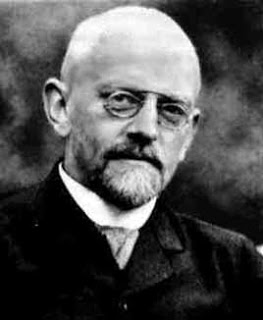
\includegraphics[width=0.50\textwidth]{hilbert}
\end{center}
\end{figure}

\lettrine{D}{avid Hilbert} was a great German mathematician. What I
appreciate the most about him is his quixotic personality and
single-mindedness, going along with Bertrand Russel on their
impossible quest to clean mathematics of all doubt and uncertainty,
always searching for strict solutions through pure thought.

In 1900, Hilbert came up with a list of 23 fundamental problems, many
of which are still being investigated to this day. In 1930, Hilbert
finished a famous speech in K{\"o}nigsberg with the words ``We must
know, we shall know'', a phrase that fits perfectly the life-long
devotion he had for mathematics.

\chapter{Interview: Federico Mena-Quintero}

\epigraph{Gnome is People.}{Luis Villa}

\begin{flushright}
  \emph{Wednesday, October 03, 2007}
\end{flushright}

Pretty much anyone who is involved with Free Software~--- even just as
a lowly user like myself~--- has heard of Federico. His blog is a
source of insightful ideas on Gnome, and lately, on performance~---
combined with a healthy dose of interest in politics and, more
importantly, good food. I decided to send a few questions to Federico,
mainly on the topics I was most curious about, and he kindly replied
to my questions~--- and did so in record time! Many thanks to Federico
for taking time off his busy hacking schedule for this interview.

\bigskip

\emph{You are one of the founders of the Gnome project, which is
  currently celebrating ten years of existence. On a recent interview
  you gave to Fosdem, you considered the platform to be
  maturing. However, as we all know, the last 10\% normally take 90\%
  of the time, and it's considered to be boring work. What do you
  think the Gnome project needs to do to get people to focus on those
  remaining 10\%?}

\bigskip

Basically, to provide an incentive to get that last 10\% of the work
done :) Instead of smacking people with a stick for not writing
documentation, you could have a web page with a bar chart of
``percentage of documentation coverage''. Then it becomes a competition:
use a carrot instead of a stick.

I'd also like companies to get more involved in this. If they want to
ship Gnome as a development platform they support, then they could
very well employ people to do those missing bits.

\bigskip

\emph{You have been one of the champions of performance in Gnome for a
while now. As functionality increased, Gnome started suffering more
and more from performance problems, particularly when looked at from a
low end perspective. You have been trying to explain to the masses
that performance work is interesting. What do you think can be done to
increase developer focus on this neglected area?}

\bigskip

The thing about fixing performance problems is that nobody teaches you
how to do it. There is very little documentation out there on how to
generically approach an optimization problem (I intend to do something
about this, but oh, time, time, time!) :)

Also, sometimes you fix a performance problem, but it reappears in the
future. This happens when you don't leave an infrastructure in place
to let you run a benchmark periodically. You need to be able to see if
there are performance regressions.

Our tools are slowly getting better, but there are really very few
people working on optimization and profiling tools. It takes a
\emph{ton} of time and skill to write a good tool; maybe that's why
there are so few of them.

Finally, profiling and optimizing is really about following the
scientific method (``make a hypothesis, change one thing at a time,
measure, confirm your hypothesis, etc.''). This requires discipline and
a lot of patience.

Basically, it's a problem of education :)

\bigskip

\emph{Earlier on this year, Gnome users and developers met for
GUADEC. Did you find the conference as productive as in previous
years? How important is GUADEC for the Gnome user and developer
community?}

\bigskip

Yes, this GUADEC was tremendously productive! I think the venue helped
a lot; the Birmingham Conservatoire is rather compact and has nice
practice rooms that anyone can use. So, you could grab a couple of
hackers and go to a room to hack peacefully.

GUADEC has always been important, even more so now that our community
is large and widespread. It is about the only time in the year when
most of the Gnome contributors get together in a single place and are
able to talk in person. Do not underestimate the productivity of
talking over a beer :)

\bigskip

\emph{From the outside world, it appears Novell is a company who has
regained it's soul and direction with Linux. How was the transition
from Ximian into Novell?}

\bigskip

Like all acquisitions, it was a bit rought at first. It's what you get
when you switch from being in a small company where you know all of
the employees, to one with several thousands of people. You have to
adjust to bigger processes, more layers of management, new locations,
new paperwork\ldots

It has been very interesting to see the mindset of the old-time Novell
people change over time. At first they seemed reluctant to touch Linux
and free software, since they were of course Windows users. Then we
had a period with lots of questions, lots of bugs that needed to be
fixed, lots of re-training\ldots and now we are in a very nice period,
when people have accepted that we must all use our own free
software. People seem to be productive with it and happy.

I miss the monkeys, though.

\bigskip

\emph{You are currently telecommuting from Mexico, a position envied by a
most developers out there. Do you find that telecommuting helps
improving your productivity? Are there any downsides to it?}

\bigskip

It has good things and bad things. Good things: working in your
pajamas if you feel like it, not having to commute, taking a pause
when you are stuck in a hard problem to do a bit of gardening. Bad
things: you can't talk to people in person. You must fix all your
networking problems yourself. Sometimes, when you are uninspired, it's
nice to be able to look over someone else's shoulder or talk to them.

\bigskip

\emph{Can you describe your typical day at work?}

\bigskip

Well, since I work from home\ldots :)

I wake up. If my wife and I are hungry, we make breakfast while my
email gets downloaded. If we are not hungry, I'll just check for
super-urgent email and then start programming (fixing bugs, doing new
development, reviewing patches, etc.).

I usually try to get some programming done in the morning, while my
brain is fresh. Processing your email in the morning is a really bad
idea; it will take you up to the afternoon and by then you'll be tired
to really write code.

We have lunch at really irregular hours. Sometimes it's more like an
early dinner. I have the bad habit of not stopping working until I'm
exhausted or my wife is angry that we haven't gone out to the
supermarket yet, but I'm trying to fix that :)

In the afternoon I tend to do ``light'' work\ldots maintaining wikis,
answering email, coordinating people. I don't really have a fixed work
schedule.

\bigskip

\emph{Many developing countries are increasingly looking at Free
  Software as a way to bring down the digital divide. Do you find that
  Mexico is taking advantage of Free Software~--- particularly since it
  has two lead Free Software developers? Are there any lessons to be
  learned from Mexico's experience?}

\bigskip

Mexico is blessed and cursed to be so close to the USA. There is
plenty of basic usage of free software by individuals (often
enthusiastic students), but relatively little usage in the public and
private sectors.

People in Mexico get very impressed by rich people; most Mexicans want
to be like the rich people from the USA they see on TV. It's very easy
to woo us into accepting their ways.

So, every time there has been some noise about using free software in
the public sector, Bill Gates has flown down, organized a big business
lunch with government officials, and made sure that they keep using
Microsoft products. If you are an ignorant politician, you will love
to gloat that you had lunch (imagine, lunch!) with Bill Gates, the
richest man in the world~--- and whatever he says must be correct, of
course. The problem we have is that most of our politicians don't have
the faintest idea of the economic and cultural implications of free
software, unlike those in the European Union (see the recent report on
the economic impact of free software there!).

\bigskip

\emph{Thanks for the interview!}

\chapter{.signature: Alan Perlis}

\epigraph{One man's constant is another man's variable.}{Alan Perlis}

\begin{figure}
\begin{center}
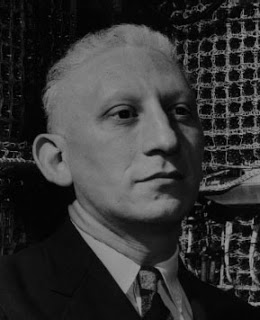
\includegraphics[width=0.50\textwidth]{alan_perlis}
\end{center}
\end{figure}

\begin{flushright}
  \emph{Saturday, October 20, 2007}
\end{flushright}

\lettrine{A}{lan Perlis} was one of the finest specimens of the Real
Programmer breed. Back in the days where Computer Scientists didn't
exist, he and his kind were responsible for making many of the
decisions that shape our view of computers today. I'm particularly
fond of Perlis because of his views on Compuer Science:

\begin{quote}
I think that it's extraordinarily important that we in computer
science keep fun in computing. When it started out, it was an awful
lot of fun. Of course, the paying customers got shafted every now and
then, and after a while we began to take their complaints
seriously. We began to feel as if we really were responsible for the
successful, error-free perfect use of these machines. I don't think we
are. I think we're responsible for stretching them, setting them off
in new directions, and keeping fun in the house. I hope the field of
computer science never loses its sense of fun. Above all, I hope we
don't become missionaries. Don't feel as if you're Bible salesmen. The
world has too many of those already. What you know about computing
other people will learn. Don't feel as if the key to successful
computing is only in your hands. What's in your hands, I think and
hope, is intelligence: the ability to see the machine as more than
when you were first led up to it, that you can make it more.
\end{quote}

\begin{flushright}
  Source: \emph{The Structure and Interpretation of Computer
    Programs by Abelson, Sussman, and Sussman}
\end{flushright}

Unfortunately, things haven't quite turned out like Perlis would have
wanted. Besides of his many contributions to Computer Science, such as
his work on ALGOL, Perlis is very well known for his Epigrams on
Programming, of which our quote is the first one. I like this quote
because it reminds me that there can never be an ultimate truth in
programming due to our human condition.

\chapter{On Evolutionary Methodology}

\epigraph{Unix's durability and adaptability have been nothing short of
  astonishing. Other technologies have come and gone like
  mayflies. Machines have increased a thousand-fold in power,
  languages have mutated, industry practice has gone through multiple
  revolutions~--- and Unix hangs in there, still producing, still paying
  the bills, and still commanding loyalty from many of the best and
  brightest software technologists on the planet.}{ESR}

\epigraph{Unix\ldots is not so much a product as it is a painstakingly
  compiled oral history of the hacker subculture.}{Neal Stephenson}

\begin{flushright}
  \emph{Wednesday, June 11, 2008}
\end{flushright}


\section{The Impossibly Scalable System}

\lettrine{I}{f development in general} is an art or a craft, its
finest hour is perhaps the maintenance of existing systems which have
high availability requirements but are still experiencing high rates
of change. As we covered previously, maintenance in general is a task
much neglected in the majority of commercial shops, and many products
suffer from entropic development; that is, the piling on of changes
which continuously raise the complexity bar, up to a point where it is
no longer cost-effective to continue running the existing system. The
word \emph{legacy} is in itself filled with predestination, implying
old systems cannot avoid time-decay and will eventually rot into
oblivion.

The story is rather different when one looks at a few successful Free
and Open Source Software (FOSS) systems out there. For starters,
\emph{legacy} is not something one often hears on that side of the
fence; projects are either maintained or not maintained, and can
freely flip from one state to the other. Age is not only \emph{not} a
bad thing, but, in many cases, it is a remarkable advantage. Many
projects that survived their first decade are now stronger than ever:
the Linux kernel, x.org, Samba, Postgresql, Apache, gcc, gdb,
subversion, GTK, and many, many others. Some, like Wine, took a decade
to mature and are now showing great promise.

Each of these old timers has its fair share of lessons to teach, all
of them incredibly valuable; but the project I'm particularly
interested in is the Linux kernel. I'll abbreviate it to Linux or ``the
kernel'' from now on.

As published recently in a study by Kroah-Hartman, Corbet and
McPherson, the kernel suffers a daily onslaught of unimaginable
proportions. Recent kernels are a joint effort of thousands of kernel
hackers in dozens of countries, a fair portion of which working or
well over 100 companies. On average, these developers added or
modified around 5K lines per day during the 2.6.24 release cycle and,
crucially, removed some 1.5K lines per day~--- and \emph{day} here
includes weekends too. Kernel development is carried out in hundreds
of different kernel trees, and the merge paths between these trees
obeys no strictly enforced rules~--- it does follow convention, but
rules get bent when the situation requires it.

It is incredibly difficult to convey in words just how much of a
technical and social achievement the kernel is, but one is still
compelled to try. The absolute master of scalability, it ranges from
the tiniest embedded processor with no MMU to the largest of the large
systems~--- some spanning as many as 4096 processors~--- and
covering pretty much everything else in between: mobile phones,
Set-Top Boxes (STBs), game consoles, PCs, large severs,
supercomputers. It supports more hardware architectures than any other
kernel ever engineered, a number which seemingly keeps on growing at
the same rate new hardware is being invented. Linux is increasingly
the kernel of choice for new architectures, mainly because it is
extremely easy to port. Even real time~--- long considered the
unassailable domain of special purpose~--- is beginning to cave in,
unable to resist the relentless march of the penguin. And the same is
happening in many other niches.

The most amazing thing about Linux may not even be its current state,
but its pace, as clearly demonstrated by Kroah-Hartman, Corbet and
McPherson's analysis of kernel source size: it has displayed a near
constant growth rate between 2.6.11 and 2.6.24, hovering at around
10\% a year. Figures on this scale can only be supported by a
catalytic development process. And in effect, that is what Linux
provides: by getting better it implicitly lowers the entry barrier to
new adopters, which find it closer and closer to their needs; thus
more and more people join in and fix what they perceive to be the
limitations of the kernel, making it even more accessible to the next
batch of adopters.

Although some won't admit it now, the truth is none of the
practitioners or academicians believed that such a system could ever
be delivered. After all, Linux commits every single schoolboy error:
started by an ``inexperienced'' undergrad, it did not have much of an
upfront design, architecture and purpose; it originally had the firm
objective of supporting only a single processor on x86; it follows the
age-old monolithic approach rather than the ``established''
micro-kernel; it is written in C instead of a modern, object-oriented
language; its processes appear to be haphazard, including a clear
disregard for Brook's law; it lacks a rigorous Q\&A process and until
very recently even a basic kernel debugger; version control was first
introduced over a decade after the project was started; there is no
clear commercial (or even centralised) ownership; there is no
``vision'' and no centralised decision making (Linus may be the final
arbiter, but he relies on the opinions of a lot of people). The list
continues \emph{ad infinitum}.

And yet, against all expert advice, against all odds, Linux is the
little kernel that could. If one were to write a spec covering the
capabilities of vanilla 2.6.25, it would run thousands of pages long;
its cost would be monstrous; and no company or government department
would dare to take on such an immense undertaking. Whichever way you
look at it, Linux is a software engineering singularity.

But how on earth can Linux work at all, and how did it make it thus
far?

\section{Linus' Way}

\epigraph{I'm basically a very lazy person who likes to get credit for things other people actually do.}{Linus Torvalds}

The engine of Linux's growth is deeply rooted in the kernel's
methodology of software development, but it manifests itself as a set
of core values~--- a culture. As with any other school of thought,
not all kernel hackers share all values, but the group as a whole
displays some obvious homogeneous characteristics. These we shall call
Linus' Way, and are loosely summarised below (apologies for some
redundancy, but some aspects are very interrelated).

\subsection{Small is beautiful}

\begin{itemize}
\item \emph{Design is only useful on the small scale}; there is no
  need to worry about the big picture~--- if anything, worrying about
  the big picture is considered harmful. Focus on the little decisions
  and ensure they are done correctly. From these, a system will emerge
  that \emph{appears} to have had a grand design and purpose.
\item \emph{At a small scale, do not spend too long designing and do
  not be overambitious}. Rapid prototyping is the key. Think simple
  and do not over design. If you spend too much time thinking about
  all the possible permutations and solutions, you will create messy
  and unmaintainable code which will very likely going to be
  wrong. Best implement a small subset of functionality that works
  well, is easy to understand and can be evolved over time to cover
  any additional requirements.
\end{itemize}

\subsection{Show me the Code}

\begin{itemize}
\item \emph{Experimentation is much more important than theory by
  several orders of magnitude}. You may know everything there is to
  know about coding practice and theory, but your opinion will only be
  heard if you have solid code in the wild to back it up.
\item \emph{Specifications and class diagrams are frowned upon}; you
  can do them for your own benefit, but they won't sell any ideas by
  themselves.
\item \emph{Coding is a messy business and is full of
  compromises}. Accept that and get on with it. Do not search for
  perfection before showing code to a wider audience. Better to have a
  crap system (sub-system, module, algorithm, etc.) that works
  somewhat today than a perfect one in a year or two. Crap systems can
  be made slightly less crappy; vapourware has no redeeming features.
\item \emph{Merit is important, and merit is measured by code}. Your
  ability to do boring tasks well can also earn a lot of brownie
  points (testing, documentation, bug hunting, etc.) and will have a
  large positive impact on your status. The more you are known and
  trusted in the community, the easier it will be for you to merge new
  code in and the more responsibilities you will end up
  having. Nothing is more important than merit as gauged by the
  previous indicators; it matters not what position you hold on your
  company, how important your company is or how many billions of
  dollars are at stake~--- nor does it matter how many academic titles
  you hold. However, past actions do not last forever: you must
  continue to talk sense to have the support of the community.
\item \emph{Testing is crucial, but not just in the conventional
  sense}. The key is to release things into a wider population
  (``Release early, release often''). The more exposure code has the
  more likely bugs will be found and fixed. As ESR put it, ``Given
  enough eyeballs, all bugs are shallow'' (dubbed Linus'
  law). Conventional testing is also welcome (the more the merrier),
  but its no substitute for releasing into the wild.
\item \emph{Read the source, Luke}. The latest code is the only
  authoritative and unambiguous source of understanding. This attitude
  does not in anyway devalue additional documentation; it just means
  that the kernel's source code overrides any such document. Thus
  there is a great impetus in making code readable, easy to understand
  and conformant to standards. It is also very much in line with Jack
  Reeve's view that source code is the only real specification a
  software system has.
\item \emph{Make it work first, then make it better}. When taking on
  existing code, one should always first make it work as intended by
  the original coders; then a set of cleanup patches can be written to
  make it better. Never start by rewriting existing code.
\end{itemize}

\subsection{No sacred cows}

\begin{itemize}
\item \emph{Anything related to the kernel can change}, including
  processes, code, tools, fundamental algorithms, interfaces,
  people. Nothing is done ``just because''. Everything can be
  improved, and no change is deemed too risky. It may have to be
  scheduled, and it may take a long time to be merged in; but if a
  change is of ``good taste'' and, when required, provided the
  originator displays the traits of a good maintainer, it will
  eventually be accepted. Nothing can stand on the way of progress.
\item As a kernel hacker, you have no doubts that you are right~---
  but actively you encourage others to prove you wrong and accept
  their findings once they have been a) implemented (a prototype would
  do, as long as it is complete enough for the purpose) b) peer
  reviewed and validated. In the majority of cases you gracefully
  accept defeat. This may imply a turn-around of 180 degrees; Linus
  has done so on many occasions.
\item \emph{Processes are made to serve development}. When a process
  is found wanting~--- regardless of how ingrained it is or how useful
  it has been in the past~--- it can and will be changed. This is
  often done very aggressively. Processes only exist while they
  provide visible benefits to developers or, in very few cases, due to
  external requirements (ownership attribution comes to
  mind). Processes are continuously fine-tuned so that they add the
  smallest possible amount of overhead to real work. A process that
  improves things dramatically but adds a large overhead is not
  accepted until the overhead is shaved off to the bare bone.
\end{itemize}

\subsection{Tools}

\begin{itemize}
\item \emph{Must fit the development model}~--- the development model
  should not have to change to fit tools;
\item \emph{Must not dumb down developers} (i.e. debuggers); a tool
  must be an aid and never a replacement for hard-thinking;
\item \emph{Must be incredibly flexible}; ease of use can never come
  at the expense of raw, unadultered power;
\item \emph{Must not force everyone else to use that tool}; some
  exceptions can be made, but on the whole a tool should not add
  dependencies. Developers should be free to develop with whatever
  tools they know best.
\end{itemize}

\subsection{The Lieutenants}

One may come up with clever ways of doing things, and even provide
conclusive experimental evidence on how a change would improve
matters; however, if one's change will disrupt existing code and
requires specialised knowledge, then it is important to display the
characteristics of a good maintainer in order to get the changes
merged in. Some of these traits are:

\begin{itemize}
\item good understanding of kernel's processes;
\item good social interaction: an ability to listen to other kernel
  hackers, and be ready to change your code;
\item an ability to do boring tasks well, such as patch reviews and
  integration work;
\item an understanding of how to implement disruptive changes,
  striving to contain disruption to the absolute minimum and a deep
  understanding of fault isolation.
\end{itemize}

\subsection{Patches}

Patches have been used for eons. However, the kernel fine-tuned the
notion to the extreme, putting it at the very core of software
development. Thus all changes to be merged in are split into patches
and each patch has a fairly concise objective, against which a review
can be performed. This has forced all kernel hackers to \emph{think}
in terms of patches, making changes smaller and concise, and splitting
scaffolding and clean up work and decoupling features from each
other. The end result is a ridiculously large amount of positive
externalities~--- unanticipated side-effects~--- such as technologies
that get developed for one purpose but find uses that were never
dreamt of by their creator. The benefits of this approach are far too
great to discuss here but hopefully we'll have a dedicated article on
the subject.

\subsection{Other}

\begin{itemize}
\item \emph{Keep politics out}. The vast majority of decisions are
  taken on technical merits alone, and very rarely for political
  reasons. Sometimes the two coincide (such as the dislike for binary
  modules in the kernel), but one must not forget that the key driver
  is always the technical reasoning. For instance, the kernel uses the
  GNU GPL v2 purely because its the best way to ensure its openness, a
  key building block of the development process.
\item \emph{Experience trumps fashion}. Whenever choosing an approach
  or a technology, kernel hackers tend to go for the beaten track
  rather than new and exciting ones. This is not to say there is no
  innovation in the kernel; but innovators have the onus of proving
  that their approach is better. After all, there is a solid body of
  over 30 years of experience in developing UNIX kernels; its best to
  stand on the shoulders of giants whenever possible.
\item \emph{An aggressive attitude towards bad code}, or code that
  does not follow the standards. People attempting to add bad code are
  told so in no uncertain terms, in full public view. This discourages
  many a developer, but also ensures that the entry bar is raised to
  avoid lowering the signal-to-noise (S/N) ratio.
\end{itemize}

If there ever was a single word that could describe a kernel hacker,
that word would have to be ``pragmatic''. A kernel hacker sees
development as a hard activity tht should remain hard. Any other view
of the world would result in lower quality code.

\section{Navigating Complexity}

Linus has stated in many occasions he is a big believer of development
by evolution rather than the more traditional methodologies. In a way,
he is the father of the evolutionary approach when applied to software
design and maintenance. I'll just call this the evolutionary
methodology (EM) by want of a better name. EM's properties make it
strikingly different from everything that has preceded it. In
particular, it appears to remove most forms of centralised
control. For instance:

\begin{itemize}
\item it does not allow you to know where you're heading in the long
  run; all it can tell you is that if you're currently on a favourable
  state, a small, gradual increment is \emph{likely} to take you to
  another, slightly more favourable state. When measured in a large
  timescale it will appear as if you have designed the system as a
  whole with a clear direction; in reality, this ``clearness'' is an
  emergent property (a side-effect) of thousands or small decisions.
\item it exploits parallelism by trying lots of different gradual
  increments in lots of members of its population and selecting the
  ones which appear to be the most promising.
\item it favours promiscuity (or diversity): code coming from anywhere
  can intermix with any other code.
\end{itemize}

But how exactly does EM work? And why does it seem to be better than
the traditional approaches? The search for these answers takes us
right back to the fundamentals. And by ``fundamentals'', I really mean
the absolute fundamentals~--- you'll have to grin and bear, I'm
afraid. I'll attempt to borrow some ideas from Popper, Taleb, and
Dawkins to make the argument less nonsensical.

That which we call reality can be imagined as a space with a really,
really large number of variables. Just how large one cannot know, as
the number of variables is unknowable~--- it could even be infinite~---
and it is subject to change (new variables can be created; existing
ones can be destroyed, and so on). With regards to the variables
themselves, they change value every so often but this frequency
varies; some change so slowly they could be better describbed as
constants, others so rapidly they cannot be measured. And the
frequency itself can be subject to change.

When seen over time, these variables are curves, and reality is the
space where all these curves live. To make matters more interesting,
changes on one variable can cause changes to other variables, which in
turn can also change other variables and so on. The changes can take
many forms and display subtle correlations.

As you can see, reality is the stuff of pure, unadulterated complexity
and thus, by definition, any attempt to describe it in its entirety
cannot be accurate. However, this simple view suffices for the
purposes of our exercise.

Now imagine, if you will, a model. A model is effectively a) the
grabbing of a small subset of variables detected in reality; b) the
analysis of the behaviour of these variables over time; c) the issuing
of statements regarding their behaviour~--- statements which have not
been proven to be false during the analysis period; d) the validation
of the models predictions against past events (calibration). Where the
model is found wanting, it needs to be changed to accommodate the new
data. This may mean adding new variables, removing existing ones that
were not found useful, tweaking variables, and so on. Rinse,
repeat. These are very much the basics of the scientific method.

Model are rather fragile things, and its easy to demonstrate
empirically why. First and foremost, they will always be incomplete;
exactly how incomplete one cannot know. You never know when you are
going to end outside the model until you are there, so it must be
treated with distrust. Second, the longer it takes you to create a
model~--- a period during which validation is severely impaired~---
the higher the likelihood of it being wrong when its ``finished''. For
very much the same reasons, the larger the changes you make in one go,
the higher the likelihood of breaking the model. Thirdly, the longer a
model has been producing correct results, the higher the probability
that the next result will be correct. But the exact probability cannot
be known. Finally, a model must endure constant change to remain
useful~--- it may have to change as frequently as the behaviour of the
variables it models.

In such an environment, one has no option but to leave certainty and
absolutes behind. It is just not possible to ``prove'' anything, because
there is a large component of randomness and unknown-ability that
cannot be removed. Reality is a messy affair. The only certainty one
can hold on to is that of fallibility: a statement is held to be
possibly true until proven false. Nothing else can be said. In
addition, empiricism is highly favoured here; that is, the ability to
look at the data, formulate an hypothesis without too much theoretical
background and put it to the test in the wild.

So how does this relate to code? Well, every software system ever
designed is a model. Source code is nothing but a set of statements
regarding variables and the rules and relationships that bind them. It
may model conceptual things or physical things~--- but they all
inhabit a reality similar to the one described above. Software systems
have become increasingly complex over time~--- in other words, taking
on more and more variables. An operative system such as multics,
deemed phenomenally complex for its time, would be considered normal
by today's standards~--- even taking into account the difficult
environment at the time with non-standard hardware, lack of experience
on that problem domain, and so on.

In effect, it is this increase in complexity that breaks down older
software development methodologies. For example, the waterfall method
is not ``wrong'' per se; it can work extremely well in a problem
domain that covers a small number of variables which are not expected
to change very often. You can still use it today to create perfectly
valid systems, just as long as these caveats apply. The same can be
said for the iterative model, with its focus on rapid cycles of
design, implementation and testing. It certainly copes with much
larger (and faster moving) problem domains than the waterfall model,
but it too breaks down as we start cranking up the complexity
dial. There is a point where your development cycles cannot be made
any smaller, testers cannot augment their coverage, etc. EM, however,
is at its best in absurdly complex problem domains~--- places where
no other methodology could aim to go.

In short, EM's greatest advantages in taming complexity are as
follows:

\begin{itemize}
\item \emph{Move from one known good point to another known good
  point}. Patches are the key here, since they provide us with small
  units of reviewable code that can be checked by any experienced
  developer with a bit of time. By forcing all changes to be split
  into manageable patches, developers are forced to think in terms of
  small, incremental changes. This is precisely the sort of behaviour
  one would want in a complex environment.
\item \emph{Validate, validate and then validate some more}. In other
  words, Release Early, Release Often. Whilst Linus has allowed
  testing and Q\&A infrastructure to be put in place by interested
  parties, the main emphasis has always been placed in putting code
  out there in the wild as quickly as possible. The incredibly diverse
  environments on which the kernel runs provide a very harsh and
  unforgiving validation that brings out a great number of bugs that
  could not have possibly been found otherwise.
\item \emph{No one knows what the right thing is, so try as many
  possible avenues as possible simultaneously}. Diversity is the key,
  not only in terms of hardware (number of architectures, endless
  permutations within the same architecture, etc.), but also in terms
  of agendas. Everyone involved in Linux development has their own
  agenda and is working towards their own goal. These individual
  requirements, many times conflicting, go through the kernel
  development process and end up being converted into a number of
  fundamental architectural changes (in the design sense, not the
  hardware sense) that effectively are the superset of all
  requirements, and provide the building blocks needed to implement
  them. The process of integrating a large change to the kernel can
  take a very long time, and be broken into a sequence of never ending
  patches; but many a time it has been found that one patch that adds
  infrastructure for a given feature also provides a much better way
  of doing things in parts of the kernel that are entirely unrelated.
\end{itemize}

Not only does EM manage complexity really well but it actually thrives
on it. The pulling of the code base in multiple directions makes it
stronger because it forces it to be really plastic and
maintainable. It should also be quite clear by now that EM can only be
deployed successfully under somewhat limited (but well defined)
circumstances, and it requires a very strong commitment to
openness. It is important to build a community to generate the
diversity that propels development, otherwise its nothing but the
iterative method in disguise done out in the open. And building a
community entails relinquishing the traditional notions of ownership;
people have to feel empowered if one is to maximise their
contributions. Furthermore, it is almost impossible to direct this
engine to attain specific goals~--- conventional software companies
would struggle to understand this way of thinking.

Just to be clear, I would like to stress the point: it is not right to
say that the methodologies that put emphasis on design and centralised
control are wrong, just like a hammer is not a bad tool. Moreover, its
futile to promote one programming paradigm over another, such as
Object-Orientation over Procedural programming; One may be superior to
the other on the small, but on the large~--- the real world~--- they
cannot by themselves make any significant difference (class libraries,
however, are an entirely different beast).

I'm not sure if there was ever any doubt; but to me, the kernel proves
conclusively that the human factor dwarfs any other in the production
of large scale software.

\chapter{On the UbuntuBox}

\epigraph{Chrome is, make no mistake, a dagger poised over Microsoft's
  heart. The only question is whether it's made of steel or rubber.}{Charles Arthur}

\begin{flushright}
  \emph{Thursday, June 19, 2008}
\end{flushright}

\section{The Regular User}

\lettrine{A}{s with many other geeks}, I find myself in the unofficial
position of ``computer guy'' for family and friends (F\&F). This
entails sorting out broken computers, providing advice on new
purchases for a variety of devices and software packages, installing
said devices and packages, doing security updates and giving security
advice, providing mini-tutorials on applications, teaching basic
programming~--- the list goes on and on. The funny thing is, much like
all other nerds, I may moan about my duties but secretly I enjoy
performing them. Sometimes I get to setup people with cheap Ubuntu
boxen, which they may complain about a little in the beginning but
eventually use in extremely productive ways; and even on windows
setups, I get to understand what drives people to Microsoft and what
its weak and strong points are. Its a very instructive job.

Things got even more interesting since I bought my eee PC, a device
that is selling like fire in the polar winter. The eee PC helped me
understand a bit better how most people think. All along we, the Linux
community, have focused on providing a user experience that is very
similar to Windows: you may not have a Start Menu but you have the
Ubuntu logo; toolbars and menus are very similar and so on. Even the
newest eye-candy is similar to Mac and Vista's way of doing things
(although there's always the chicken-and-egg problem). The end result
is interesting: developers and regular Linux users are now convinced
that no one should have any difficulties at all moving from Windows to
KDE or Gnome; on the other hand, as soon as you sit a user down on a
Linux box, he or she immediately tells you that something is not
right. Objectively, the average user will probably not be able to
point out what's wrong, if anything at all, other than ``this is not
Windows, can we not have Windows please''.

The fantastic thing about the eee PC was that, of all people I showed
it to, not a single one said: bah, this is not Windows. Most of them
got on with the user interface immediately, and found it really
intuitive. In all my years of advocating Linux I never before seen a
reaction like this. I did absolutely no advocating whatsoever, no
mention about freedom or the superiority of free software. Just
letting them play with it was enough. As an example, my girlfriend has
been using Linux for over 5 years, and I get the periodic complains of
``why can't we just use windows'' whenever I have some difficulties
installing a device, or I break the world on a dist-upgrade. But
within minutes of playing with the eee, her reaction was: ``I want one
of these!!''.

The reactions I've seen towards the eee PC are almost the opposite of
the few Vista users I've spoken to. Sure, Vista looks nice, but have
you tried installing a one-click wireless router? That's when F\&F call
me out, when it all goes wrong with the ``one-click'' cheap product they
bought. But thing is, I can't say much in Ubuntu's defense either. For
example, I spent several days installing a Huawei e220 modem to
provide 3G Internet access to my nephews, and let me just tell you,
trivial would not have been a word one could apply to any part of the
process. Vodaphone's new clever GUI may be good for Vodaphone users
but I never got the damn thing to cooperate. True, the whole exercise
wasn't taxing for a nerd~--- hey, its fun to look at AT commands now and
then~--- but there is no way, just noooo waaaay a regular user would
have gone through the pain, even with the brilliant Ubuntu forums to
hand.

Now, before we go any further, I can already hear the complaints: ``so
you've chatted to what, twenty people, and now you think you
understand the market?''. Well, that much is true, I cannot claim any
statistical accuracy to my diagnostics. These are my opinions; the
entire article is based on empiricism and small samples. However, if
my line argumentation is done correctly and rightly interprets the
success of the eee, then there must be some truth to my views because
I've tried to align them with the eee. The market has given a verdict
on this gadget, loudly and unequivocally.

The eee PC is also a brilliant illustration of the huge divide between
regular users and the developers who are tasked with providing
software for them. At a moment in time where the Gnome community is
yet again rethinking the future of Gnome, not a single regular user
would find this debate interesting. This should send all the alarm
bells ringing, but unfortunately that doesn't seem to be the case. The
truth is, regular users don't want flashy 3D desktops, although they
can eventually cope with them; they don't need spinning cubes although
they may start using them once they understand it. What they really
want is simplicity. They have a simple set of tasks to perform, and
they want to do so cheaply and reliably, and they truly do not
understand why everything has to be so complicated and why do
computers have to change so much so often.

So what made the eee popular? In my opinion, there are two key points:

\begin{itemize}
\item its cheap. No one would even have a look at it if it was 400 GBP
\item its easy.
\end{itemize}

These are the key selling points to a regular user. To illustrate the
second point, when I said to my girlfriend I was thinking about
installing Ubuntu Hardy on the eee, she replied in dismay: ``Why would
you do that??''.

\section{The Regular User Use Cases}

The key thing to notice about the eee is that most users don't even
know its not running Windows. Its just an appliance, a bit like a
PlayStation, and thus there is no need to enquire about it's operative
system. Like an appliance, it is also expected to be switched on and
just work~--- the fast boot reinforces this idea. The interface
provided is also designed for the tasks common to the vast majority of
regular computer users, and allows them to find things fast. But,
looking at the wider problem, what do our regular users do with their
computers?  I compiled a list of all use cases I found in my user
base:

\begin{itemize}
\item Internet: email, browsing, playing on-line games and youtube;
\item Listen to music, sync with their music player;
\item Watch local video content;
\item Talk with their friends: IM, VOIP
\item Play (basic) games: on all cases, real gaming is done on the
  PlayStation;
\item Work: word-processor by far, some spreadsheet use but ``it's
  quite hard'';
\item Burning and ripping;
\item Downloading: torrents, etc. Not very popular because ``its
  complicated'';
\item Digital photo management: storage, some very basic manipulation
  (make it smaller for emailing);
\item Printing: mainly for school/University; pictures in very few
  cases.
\end{itemize}

In addition to these, some additional requirements crop up:

\begin{itemize}
\item Windows users all have proprietary firewalls and virus scanners;
\item All machines are multi-user, and data must be kept private~---
  especially with the youngsters;
\item Machines must withstand battering: switched off at any point,
  banged about, dropped, etc;
\item Internet connectivity is vital, ADSL, cable and 3G are
  used. Computers are useless without the Internet;
\item Wireless around the house is vital. External wireless is nice,
  but not frequently used because ``it's too complicated'';
\item Costs must be kept exceedingly low as IT budget is normally very
  low;
\end{itemize}

That's it. You'd be amazed with the percentage of the market one
covers with only these use cases; not just doing them, but doing them
well, like a PlayStation plays games.

And what are the biggest complaints about computers?

\begin{itemize}
\item They're really hard. Installing hardware and software is a
  nightmare, and they'd be stuffed without the local nerd;
\item They break easily. One of my Vista users is still in disbelief
  that installing wireless drivers could cause the DVD drive to stop
  working;
\item They're expensive. Sure you can get a cheap'ish box but then
  everything else is expensive (software, peripherals, etc);
\item They change far too frequently. Most users just about got around
  XPs user interface just to see it all change again;
\item They're insecure. They don't know how or why but that's what
  they've heard. That and the constant popups that look like viruses.
\end{itemize}

On one hand, the regular user is quite advanced, making multi-user and
networking a central part of its computer experience. On the other
hand, he/she is very naive: the vast majority of computing power goes
under-utilised~--- the OS gobbling most of the resources for no good
reason~--- and the majority of software expenses easily avoidable by
using freely available applications. Regular users haven't got nowhere
near using Media Centres, ``clever'' media management software, or
even connecting their PCs to the TVs. All these things they consider
``advanced'' and yet nerds and more savvy users have been doing it for
years. One cannot help but feel that there is a massive market out
there for the taking~--- a market that Vista cannot aim to grab
because it's diametrically opposed to its needs~--- and yet, no one
else seems to find the path to its door.

\section{UbuntuBox: The Hardware Platform}

The rest of this article is an Ubuntero Gedankenexperiment: if I was a
manufacturer, what sort of box would I like my F\&F to have? What would
make my life and their life easier? The short answer to that question
is a PlayStation 2 like box but with PC-like functionality. The long
answer is, well, long.

I'm not going to bother with engineering reality here~--- I'm sure
some requirements will be so conflicting they cannot possibly be
implemented. However, I've got zero experience in hardware
manufacturing, weights, cooling, large scale deployment and so on~---
so much so that I'm not even going to bother pretending; any
assumptions I'd make would be wrong anyway. So, to make matters easy,
I'll just ask for it all~--- impossible or not~--- and wait for the
reality check to come in.

The first, very different thing about our box is that it's not a
computer. Well, inside it is a regular PC of course, but it doesn't
look like one. It is designed to look exactly like a DVD player, and
to fit your living room. A bog-standard black-box with a basic LED
display would do. Inside, it has:

\begin{itemize}
\item Multiple cores: four would be ideal, but at least two. They
  don't have to be particularly fast (1.x Ghz would do, but I guess 2
  Ghz would be easier to find);
\item 4 GB of RAM: can be the slowest around, but we need at least 4;
  the more the merrier, of course;
\item 250 to 500 GB hard drive: the more the merrier. Doesn't have to
  be fast, we just need the space;
\item Average video card: key things are RGB/HDMI and TV out;
  resolution decent enough to play most games (not the latest);
\item Loads of USB ports;
\item RW DVD drive;
\item Analog TV + DVB card (for FreeView in England);
\item Wired and Wireless Ethernet;
\item Sound card with 5.1 surround sound: doesn't have to be a super
  card, just an entry level one would do;
\item SD card, compact flash readers;
\item Ability to control the box with a remote control;
\end{itemize}

And now the key limiting factor:

\begin{itemize}
\item The overall cost of the box must not exceed 200 GBP. This may
  require some tweaking, e.g. if raising it to 299 means we can put
  all features in, it may be worthwhile.
\end{itemize}

Notice that all the hardware will be standard on all boxes of the same
generation. This is all commodity hardware~--- certainly nothing
proprietary~--- but without the heterogeneity that is associated with
it. Note that control is a key feature~--- the limiting of user and
vendor freedom to swap things at will. We'll return to the topic later
on, as I'm sure it will prove controversial.

Now, how does the box behave for the regular use case? Well, you buy
it, plug it in, set all the cables up and start it up. You will see
only two things on boot: the logo (say the Ubuntu logo) fading in and
out, and the console password. That's it. No BIOS, no flashing
X-Server, nothing else. Within a few seconds you'll be prompted for
the console password and given an option of not needing a password in
the future (Note: console is \emph{not} root). Lets leave the desktop at
that for the moment as we'll cover it properly in the next section.

What about Internet access, you ask? Well, you will need to buy one of
the available modems:

\begin{itemize}
\item 3G;
\item ADSL;
\item Cable.
\end{itemize}

Each of these modems are made available at market prices (i.e. as
cheap as possible); however, they will have been officially and
exhaustively tested and stamped with a ``UbuntuBox compliant vX'' or
some such, where vX is the box's generation. To be compliant means
that your hardware has been throughly tested and is known to work with
the hardware and software in a given generation. When you plug any of
these devices after console login, a simple wizard will appear asking
you to choose a provider. Each provider will have been also part of a
certification program before inclusion.

The other networking device is an Ethernet Switch. This is only
required if your modem does not come with switching abilities (maybe
in the 3G case). Network Manager already does a pretty good job of
this, so all you'll need to do is setup the network on your console
session (SSID, etc). You can use a USB keyboard for this or just
endure typing from the remote control.

Note that the certification requirement is extended to all hardware
used with the box. In other words, there is a pretty draconian control
on the hardware platform. Users are, of course, free to do as they
wish with the device they bought, but if they go down the uncertified
route, all support contracts are rendered void (more on this
later). The truth is, its impossible to provide cost-effective support
to all possible permutations of off-the-shelf hardware~--- a fact all
Linux and Windows nerds are all too aware, as are Mac engineers. There
will always be some weird combination that makes things break, and it
can take many, many man-days to fix it; when you have 1M boxen out
there, this cost would be prohibitive. The only way is to control the
standard platform.

For all of its closeness, the certification process is actually open
when compared with other companies. All the criteria involved is made
available in public websites, APIs with all the hooks required to
extend wizards are public (with examples), companies are free to do
public dry runs and any company can request a slot for
validation. Perhaps some cost needs to be associated with the process
(time is money after all, and we must discourage the less serious
companies), but in general, the process is fair and public. The tests,
however, are stringent; hardware that passes \emph{cannot} fail when
deployed in the wild.

One final note with regards to entry level hardware. Some people may
not be aware, but the computing power available as standard today is
incredibly high. For example, one of the PCs I maintain has a 1Ghz
CPU, 512 MB of ram, 10 GB hard drive and an average ATI card; I bought
it for 60 GBP. This machine runs Ubuntu Hardy and sometimes has to
cope with as many as 3 users logged on. It doesn't do any of the 3D
Compiz special effects due to the dodgy ATI card, but it does pretty
much everything else. You'd be surprised on what you can do with the
slowest RAM, cheapest sound-card and so on.

\section{UbuntuBox: The Software Platform}

By now you must have guessed that the box would be running Ubuntu; but
this is not your average Ubuntu. Using an interface along the lines of
Remix, we would make a clear statement that this is an appliance~---
not a PC. As the eee has demonstrated, perceptions matter the
most. Remix's interface will remind no one of Windows, whilst at the
same time making the most common tasks really easy to locate.

In addition to regular Ubuntu, the software platform would provide,
out-of-the box, complete media support. This entails having GStreamer
will all the proprietary plugins, Adobe's flash and any other plug-ins
that may be required for it to play all the media one can throw at it.

The UbuntuBox is mainly a clever Media Centre, and, as such,
applications such as Elisa, Rhythmbox/Banshee, F-Spot, etc are at the
core of the user experience. These applications would need to be
modified slightly to allow for a better multi-user experience
(e.g. shared photo/music collections, good PVR and DVB support, etc),
but on the whole the functionality they already provide is more than
sufficient for most users.

As with the hardware side, the software platform is tightly
controlled. Only official Ubuntu repositories are allowed, and all
software is tested and known to work with the current generation of
boxen. And, as with hardware, the software platform is made available
for third-party who want to deploy their wares. An apt interface
similar to click 'n run is made available so that commercial companies
can sell their wares on the platform and charge for it. They would
have to go through compliance first, of course, but if the number of
boxes out there is large enough, there will be companies interested in
doing so. This would mean, for example, that a games market could
begin to emerge based on Wine; instead of having each user test each
Windows application for their particular setup, with many users having
mixed results, this would put the onus of the testing on the company
owning the platform and on the software vendor. Games would have to be
repackaged as debs and be made installable just like any other Debian
package. Of course, the same logic could be applied to any windows
Application.

As I mentioned previously, boxen come with support contracts. A
standard support contract should provide:

\begin{itemize}
\item Access to all security fixes;
\item Troubleshooting of problems, including someone remotely
  accessing your machine to help you sort it out.
\end{itemize}

Due its homogeneity, UbuntuBox is very vulnerable to attacks. If an
exploit is out in the wild, large number of boxen can be compromised
very quickly. To make things a bit safer, the platform has the
following features:

\begin{itemize}
\item SELinux is used throughout;
\item All remote access is done via SSH and is only enabled on demand
  (e.g. when tech support needs access);
\item All users have passwords and must change them regularly;
\item There is an encrypted folder (or vault) for important documents,
  available from each user's desktop.
\end{itemize}

Finally, notice that binary drivers and proprietary applications are
avoided when possible~--- e.g. Intel drivers would be preferable to
nVidia, provided they have the same feature-set. However, where the
proprietary solutions are technically superior, they should be
used. Skype springs to mind.

\section{UbuntuTerm}

By now you must be wondering, ``this is all very nice and dandy, but
am I supposed to do my word processing using a TV?''. Well, not
quite. Whilst the TV is central, its use is focused on the gaming and
Media Centre aspects of the box. If you want to use UbuntuBox as a
regular PC, you will need to buy a UbuntuTerm. Just what is a
UbuntuTerm? It is a dumb terminal of ``old'' in disguise
(e.g. LTSP). It is nothing but a LCD display of a moderately decent
size (19" say), with an attached PC~--- the back of the monitor or the
base would do, as the hardware is minimal. The PC has a basic single
core chip with low power consumption to avoid fans and on-board video,
sound and wireless Ethernet. It is designed to boot off the network if
BOOTP can be used over wireless; if not, from flash. Whichever way it
boots, its configured to find the mothership and start an XDMCP
session on it. Its price should hover around the 100 GBP mark.

As with any decent terminal these days, UbuntuTerm is designed to fool
you in believing you are sitting on the server. X already does most of
the magic required, but we need to take it one level further: if you
start playing music, the audio will come out of your local speakers
via pulseaudio; if you plug your iPod via its USB port, the device
will show up on your desktop; if you start playing a game, the FPSs
you get remotely will comparable to playing it on the server. As with
everything else mentioned in this article, all of these technologies
are readily available on the wider community; its a matter of
packaging them in a format that regular users can digest (see Dave's
blog for example).

The standard hardware on a UbuntuTerm is as follows:

\begin{itemize}
\item Low RAM, basic video card;
\item Speakers attached to monitor;
\item SD Card, compact flash readers;
\item WebCam, headset;
\item Lots of USB ports
\end{itemize}

A house can have as many UbuntuTerms as required, and the server
should easily cope with at least 6 of them without too much trouble,
depending on what sort of activities the users get up to.

\section{Conclusions}

UbuntuBox is an attempt to ride the wave of netbooks; it also tries to
make strengths out of Linux's weaknesses. The box is not may not live
up to everyone's ideals of Free Software, but its main objective is to
increase Ubuntu's installed base, allowing us to start applying
leverage against the hardware and software manufacturers. The design
of the box takes into account the needs of a very large segment of the
market which have basic computing needs, but don't want to became
experts~--- just like a PlayStation owner does not want to know the
ins-and-outs of the PowerPC chips.

The UbuntuBox is an appliance, and as such is designed to be used in a
fairly rigid number of ways, but that cannot be avoided if one wants
to stay true to its nature. The more freedom one gives to users, the
worse the end product will be for the Regular User, which cares not
for intricate technical detail.

Note also I haven't spent much time talking about business models for
the company providing UbuntuBoxen. The opportunities should be there
to create a sustainable business, based on revenue streams such as
monthly payments for support, fees from OEMs, payments to access the
platform (content providers). However, I don't know too much about
making money so I leave that as an exercise to the reader.

All and all, if there was an UbuntuBox out there for sale, I'd buy
it. I think such a device would have a good chance of capturing this
illusive segment of the market, giving Linux a foothold, however
small, on the desktop.

\chapter{2009: Year of World Domination?}

\epigraph{Ninety-Ninety Rule: n. The first 90\% of the code accounts for
  the first 90\% of the development time. The remaining 10\% of the
  code accounts for the other 90\% of the development time.}{Jargon}

\begin{flushright}
  \emph{Sunday, February 1, 2009}
\end{flushright}

\section{World Domination Revisited}

\lettrine{I}{t's hard to believe}, but it has been almost two years
since I ranted on World Domination. Two years have rolled by, and it
seems appropriate to resume the theme, but from a slightly different
angle.

So, lets cut to the chase. Will 2009 be the Year of the Linux Desktop?
The short answer is no, and I think its now clear it will apply to
2010, 2011 and so on. In fact, in 2009 we won't even meet the looser
definition of World Domination I proposed, although we're getting
closer.

What has happened since 2007? Well, we became a lot more popular in
the desktop segment, in particular on the whole new category ofMIDs
and netbooks; at one point we entirely dominated it, but over time
normal computing trends reasserted themselves. According to the latest
figures, Linux now ships on around 10-15\% of newnetbooks, as opposed
to the incredible 100\% we had in the beginning. Netbooks had the
highest visibility, but, to be fair, some inroads were made on all
usual areas including server and regular desktop markets. Good, but
nothing jaw dropping.

So we find ourselves, two years later, asking ourselves the age old
questions. Why haven't we seen at least one significant large
migration? Why didn't one of the multinational companies punt on a
100K RedHat or Novell desktop migration?

\section{A Maturing Industry}

For those who, like me, have been using Linux for over a decade, there
always has been a lingering feeling, an idea on the back of one's mind
insisting that one day the world would suddenly get it: the herd would
finally see the light and the big mass migration would
begin. Microsoft's time would come to an end, just as the once
unassailable empires of IBM and DEC eventually faded. But time has
gone by, the public has been exposed to Free Software, and yet no
major visible changes have occurred. On the plus side, all these years
of waiting gave us plenty of data points to calibrate our
understanding of the software industry. Perhaps now we can begin to
build a model that explains why things turned out the way they did.

Looking back, one of the key things one cannot fail to notice is how
the world has changed in the last twenty years. The world in which I
was brought up was a world of fast paced change, of great volatility:
companies sprung from nowhere, dominated the market and then
disappeared as if they never existed. Sinclair'sZX Spectrum,
Commodore's C-64 and Amiga, Tandy's machines and so many other brands
came and went, all in the blink of an eye. Those were heady times. It
happened during so long a period that one started to believe this was
the way of the world: a superior product immediately bought by a
significant critical mass of consumers, only to be dumped as soon as a
new leader emerged.

But the computer world was small then, and it belonged mainly to
geeks. The homebrew generation had receded into the shade a bit, to be
sure, and mass production took over; things got easier for
users. However, the target market was still tiny, and still mainly
composed of dedicated people willing to put in the hours to get things
to work.

Non-geeks~--- particularly suits~--- viewed the wild west mentality of
the technology sector in a completely different light. For them, it
was a serious problem. The technology was promising and the killer
applications were beginning to appear, but caution ruled the
day. After all, one could invest a considerable amount of money on
hardware and software, make a glorious 3 year plan with all bells and
whistles, only to find out that the vendors had folded, or gave up on
the products entirely. This was no way to run a business.

Microsoft saw it clearly and responded by talking the language
business wanted to hear. It was time for ``workgroups'' and ``solutions'',
for ``office'' and ``enterprise''. Windows 3.11 was a great step on that
direction but, SWAGing somewhat, I'd say Windows 95 was the
cornerstone. It marked the end of the wild frontier days, and signaled
the consolidation of the new world order. Microsoft's strategies, much
like those of a Machiavellian prince, were focused on stabilisation
through domination. It was nasty, but extremely effective. Their
dominance achieved what business most wanted, which was predictability
and standardisation. Here was, finally, a solid ground on which to
plan.

The result was explosive. Microsoft went from a small vendor in a
highly competitive market to the dominant force. By creating
standards~--- however closed one may consider them to be~--- the
company helped expand exponentially the overall size of the market,
and developed a vital symbiosis with business. Each release of Windows
provided both stability (through flawless backwards compatibility) and
a dazzling number of new features; and each release was delivered at a
rate which fit nicely with business' need for planning.

And so the world went, in this nice happy fashion, from Windows 95 to
Windows 98, NT 3.5, to NT 4, Windows 2000 to Windows XP. What
Microsoft managed to achieve between Windows 95 and XP was
ubiquity. Suddenly everyone everywhere was using Windows and Office,
and the numbers were huge. Immense. The geeks were finally,
completely, totally, utterly dwarfed by the non-geeks.

XP was a landmark release in more ways than one, though. It is with XP
that we meet our second inflection point, at which the symbiosis
between Microsoft and business started to breakdown. Until XP business
never really questioned the upgrade cycle: hardware grew so much
faster from one year to the next that it made perfect sense to upgrade
machines regularly. Software in itself also suffered dramatic
improvements from release to release, benefiting those who kept up
with the times. Being at the cusp of the wave was a competitive
advantage.

But with XP, strange things begun to happen:

\begin{itemize}
\item Moore's law hit a social barrier; suddenly people stopped
  wanting the fastest PCs and started looking instead for other things
  such as peripherals, bigger and better monitors, etc. And much more
  importantly, low end PCs became good enough for the vast majority of
  tasks.
\item Microsoft's products went from being seen as the cheap
  alternative to expensive brands, to the expensive brand with no real
  alternatives. The operative system cost became a significant part of
  the overall PC cost.
\item Upgrade fatigue kicked in, and many companies begun to ask just
  exactly why there was a need to change the entire estate so
  frequently.
\item The size of the PC market became so large that it just wasn't
  feasible for a large part of it to quickly upgrade as it had
  happened in the past.
\end{itemize}

In short, the PC market started showing signs of maturity. Microsoft's
objective~--- their attempt to stabilise and standardise the PC
market~--- had been achieved; but at the same time, its success may
have brought about great difficulties for the company. Seen in this
light, Vista's problems are not so much technical. There may be a
number of significant issues with the operative system~--- although most
Windows users I regularly speak to seem to be pretty happy with it. It
has its rough edges, but so did XP in the beginning and Windows 95
before it, and that didn't stop them from being huge successes.

What has changed fundamentally is the relationship between Microsoft
and its user base. There just isn't any need for mass upgrades
anymore, and the more constrained IT budgets get, the more obvious
this becomes. After all, Vista was extremely successful on the new PC
segment; it struggled more when trying to convince existing PC owners
to upgrade. I am strongly convinced that Windows 7 will suffer the
same fate. The crucial element on its adoption is going to be the End
Of Life of XP, because no business will want to run a product that is
no longer supported by its creator. When EOL is declared for XP , all
business will start to migrate to Windows 7~--- but not before
then. They are more than happy with it; it works, it's well supported
and more importantly, \emph{they know how it behaves}. The learning
curve will start from scratch, be it Vista or Windows 7, and, from a
commercial perspective, for no particularly good reason.

In truth, business need only a platform that is
\begin{inparaenum}[\itshape a\upshape)]
\item good enough (in which case they won't change)
\item compellingly better (in which case they will want to change)
\item compellingly cheaper (in which case they will be made to change
  by external pressures)
\end{inparaenum}

Its becoming harder and harder to create software that is so
compellingly better that would make users upgrade. And Microsoft
cannot start a cannibalisation strategy based on price, because its
business model is based on the notion that products become
progressively more expensive (after all their R\&D costs increase
dramatically from release to release, in the illusive search for
killer features). The only weapon left to the company is to force
customers to upgrade by whatever other means available~--- such asEOLing
products. This can only be done for so long until business wises up.

It is in the midst of this carnage that Mac and Free Software products
are competing. In view of this, one can conclude that no one~---
Microsoft included~--- will have an easy ride convincing large numbers
of existing users, business or home, to switch. The real fight for
change is going to happen on the fringes of the PC market, the beaches
where those new machines are being sold.

Here, there are two weapons available to Free Software: technological
superiority and price.

\section{Competing on Technological Superiority and Price}

A lot of nerds, to some extent myself included, are convinced that
Linux is technologically superior to Windows. In short, UNIX is
elegant and Windows is a kludge. The mystery is why no one else seems
to see this. However, when one delves a bit further, there are several
problems with the current state of Linux, and all of them are related
to the ninety-ninety rule.

The crucial difference between the business oriented approach taken by
Microsoft and other software vendors is this: its best to have
something that works somewhat now than something that works perfectly
in a few years time. With this in mind, one can spot many, many things
were developed on Windows with an almost exclusive focus on
time-to-deliver. Microsoft's engineers didn't spend months looking at
X-Windows to implement a GUI, nor did they worry aboutremoting until
they were forced to, or with shell scripting; the list goes on and
on. Now contrast that with Linux:

\begin{itemize}
\item D-Bus was years in the making, and its only now we're seeing a
  significant adoption at the application level, with many exported
  interfaces;
\item GStreamer was years in the making, and its only now we're seeing
  stability at the codec level, good support for most popular formats;
\item PulseAudio has been years in the making and we're still
  experiencing loss of sound, problems with proprietary applications,
  etc.;
\item XFree and X.Org have been years in the making and we still have
  problems with some drivers, a flickering startup on boot and on user
  switch;
\end{itemize}

The list goes on and on. From a user perspective, it matters not that
PulseAudio (to pick but one victim) is architecturally extremely well
designed and copes with an horrendously complex problem domain, made
all the more complex due to the zoo of sound solutions in Linux. What
matters is that he or she cannot useSkype to talk to their friends
because it doesn't work. Or it may work, but the instructions are so
complex that no sane non-geek could follow. Or that using Flash causes
the web browser to crash.

In general, I think it's fair to say that in places were there was
enough time to think, design, implement and stabilise a solution, Free
Software projects did a much better job than Windows; take packaging
at the distribution level for example and compare that with the amount
of clicks required to keep all windows applications
up-to-date. However, due to the very nature of Free Software
development, solutions have a tendency to take a lot longer to reach
stability. This is a good thing, because when they mature, they are
truly technical achievements.

For example, it would have been easy to slot X.Org into the kernel,
much like Windows did in the past to achieve better performance. Not
so in Linux. The long path was taken, painstakingly working out which
bits of code really needed to be in the kernel, and which should live
in X land. The end result,KMS, is amazing, and will have large amounts
of side-benefits~--- like most changes in Free Software tend to
have. But even when all KMS code has been merged, we will still have
to wait for the binary drivers to pick up these changes, so it may be
quite some time until end users see any benefits.SELinux is also
another example. Implementing the infrastructure and changing the
kernel was in itself hard; but the real toil is now being done
byRedHat and the community, spending many painstaking hours going
through applications and creating the appropriate policies. Only then
willSELinux really shine.

So, whilst I don't think, from a user perspective, that we are
superior to Windows at present, I do think that in the near future
(three years) we will be. What's more, we now have a platform for
growth and its really easy to bring companies on board. For example,
just look at dropbox and their Nautilus integration.

The Linux desktop of the future will be so uber cool its impossible to
describe. Insanely fast boots, fantastic graphical support with no
flickering from boot to desktop or on user switching, great
integration between apps courtesy of D-Bus, all sorts of weird and
wonderful sound capabilities courtesy ofPulseAudio, Telepathy for
presence, great UI in Gnome and KDE. And all because each developer
chose to take the long and hard path rather than the easy way out.

That being said, we have to live in the present, and we are still at
the point of paying the cost. Soon the second 90\% will be done.

The last topic I'd like to discuss is price. If there is something
Microsoft cannot compete on with Free Software, its on price. After
all, one can't really go much lower than zero. However, it's important
to notice that when it comes to business, cost is a tricky thing. So
much of it comes down to perception. After all, one could argue
successfully that user retraining is required to move from Windows to
Linux. This would dramatically increase the costs, making such a move
prohibitively expensive. On the same token, one could look at the
example of people such as Dave Largo, and conclude that Linux can be
easily adopted by end users with very little training, requires little
hardware and is infinitely configurable with little effort.

In truth, cost will never be an easy proposition for Linux until
technical superiority is attained. On the server side, the battle was
not ``won'' because Linux was free but because the solutions being
offered were technically superior, integrated well with Windows and
were being priced at a significant discount of a Windows
equivalent. Only then did price become significant. Something similar
needs to happen to the desktop market.

\section{Conclusion}

I hope I succeeded in demonstrating that there will never be a Year of
the Linux Desktop as such, but instead, one should expect the
continuation of present trends: a sequence of years with slow and
steady gains being made. Maturity changed the rules of the game
somewhat.

If we had the current Linux desktop a decade or so ago, when the
market was younger and more fragmented, we would probably take on a
significant share of the market, even competing againstXP . But things
changed, and there is a lot more inertia everywhere. With regards to
the battle for new computers, the key factor there will be
technological superiority. Linux will stand a good chance of fighting
for that market in the next three years, once all the core
infrastructure stabilises.

\chapter{On MinGW, Cygwin and Wine}

\epigraph{All problems in computer science can be solved by another
  level of indirection.} {David Wheeler}

\epigraph{\ldots except for the problem of too many layers of
  indirection.} {Kevlin Henney}

\begin{flushright}
  \emph{Friday, May 18, 2012}
\end{flushright}

\emph{Standard Disclaimer}: as with all posts in Nerd Food, this is a
summary of my notes and experience on the subject. Its likely there
will be incorrect bits of information so don't start building your
personal nuclear power station using this article. Or if you do, don't
blame me.

\section{UNIX Stranger on a Windows Strange Land}

\lettrine{L}{ike pretty much} every other UNIX nerd, I've been
stranded on Windows for long periods many times in my career. Whenever
that happens, cygwin is what keeps me sane and affords me a modicum of
productivity in hostile surroundings.

My relationship with Cygwin started in the long forgotten days of B19
when Men were Men and there was no setup.exe~---just archives that were
unpacked manually. I even sent a post or two to the mailing list in
those days, or so Google says. One thing I never did was to write
about how Cygwin does its magic, and that's mainly because it has just
worked for the things I needed it to do. Recently I found myself doing
some more advanced stuff and it spurred me to write a post.

Before we can understand Cygwin, we need to get some fundamentals out
of the way. However, if you came here just to get a summary of
solutions and implications without necessarily understanding the
fundamentals, feel free to jump straight to Choosing the Environment
that Fits You.

\section{The Kernel and User Space}

All operative systems share one feature in common: they all have a
kernel. The job of the average kernel is to do low-level stuff like
allowing multiple processes to share a physical machine without
getting on each others toes. The kernel does this and much, much more,
either through its core code or via dynamically loaded modules such as
the device drivers provided for your graphics card.

Kernels vary wildly in how they do things internally; that's why there
are so many different ones. Even more importantly~---at least for our
purposes~---they greatly differ on how they interface with the layers
above them, somewhat derogatorily known as the ``user space''. The
kernel exports an interface to the outside world, but this is normally
not meant to be consumed directly; instead users rely on higher-level
components to consume it. There are two sides of this interface: the
API and the ABI. Unfortunately, very frequently we use API to mean a
combination of both, but in reality there is a difference.

\section{The Kernel Application Programming Interface (API)}

When we talk about the API we normally mean a set of headers that can
be used to compile code that talks to the kernel directly. For a
simple example for the Linux kernel have a look at the Real Time Clock
Driver Test/Example Program. You can see it includes a linux kernel
header:

\begin{pseudocode}[backgroundcolor=\color{lightgray}]
#include <stdio.h>
#include <linux/rtc.h>
#include <sys/ioctl.h>
...
\end{pseudocode}

These are used to talk directly to the RTC, using standard calls such
as ioctl, etc.

\section{The Kernel Application Binary Interface (ABI)}

From a kernel perspective, its best to think of the ABI as a
specification that allows stitching together binary components. The
ABI is actually huge, and encompasses very many different aspects,
such as:

\begin{itemize}
\item the system call ABI, exemplified here for linux. It describes
  how function calls are setup, how the stack gets cleaned up after
  the function call, etc.
\item the object file format, responsible for describing the layout of
  binaries such as executables and shared libraries. Most Unices
  support ELF or the older COFF or the even older a.out; Windows uses
  PE.
\end{itemize}

Finally, one last word on internal versus external ABI. Linux tries
very hard to make sure the external ABI is kept stable; this is why
you can run the same binaries on pretty much any version of the kernel
(all things being equal, such as the presence of all dependencies
required by the binary). However, Linux makes no guarantees whatsoever
with regards to the internal ABI. This means you cannot compile device
drivers for a version of the kernel and expect them to work with other
versions; they may, but then again they may not. Windows takes the
opposite approach, trying hard not to break binary compatibility.

\section{UNIX and The C Library}

It is somewhat tautological to say that, on UNIX, the outer edge of
user space begins with the C POSIX Library. It contains all of what is
available on the C Standard Library~---that is, the library of
functions and types created for the C programming language~---and, in
addition, it also contains POSIX extensions. It may also contain other
non-standard extensions, but we'll ignore these for the sake of
simplification.

This entire package is what we commonly call the C Library. If you use
Linux you are probably using glibc, the GNU implementation of the C
Library. Furthermore:

\begin{itemize}
\item when people refer to the C runtime (CRT) they normally mean the
  shared object (or dynamically linked library) providing the binary
  implementation of the C Standard Library;
\item to link statically against the C runtime means that your
  application will contain the entire run-time rather than share one
  with other applications.
\end{itemize}

Now, its important to bear in mind that there's nothing particularly
magical about the C library; is just a set of functions defined by the
C programming language and the POSIX standardisation
process. Externally it looks like pretty much any other library. What
tends to make the C Library a bit special is that pretty much
everything on a UNIX system depends on it in one form or
another. Also, unlike other libraries, the C Library makes use of
kernel APIs to implement the interfaces it exports, and as such it
shields the layers above from the vagaries of any particular kernel.

You are probably wondering if these functions would not also be useful
to the kernel itself. After all, it is more often than not built in C,
right? Unfortunately, due to the highly circular nature of the
problem, the kernel cannot make use of the C Library. The kernel uses
what is commonly referred to as pure C; that is, only the core C
language itself. It must provide its own implementation of all
required functions, which can be inspired by code in the C library.

\section{The Windows API}

On Windows~---as always~---things are not quite as simple. The Windows
API is the equivalent outer edge of user space on Windows-land (when I
say API here, I really mean API + ABI, which is traditionally what
people mean). Instead of a nice separation of core APIs that interface
with the kernel, the Windows API appears to users as one big monolith
with many, many responsibilities all bundled together. In reality, its
actually made up of a great number of distinct libraries, but that's
not how it seems to the untrained eye.

As far as the C Library is concerned, well, it has no direct
equivalent. The C Standard Library exists on Windows, of course, but
its not seen as a core component of the operative system; its more of
a add-on which you can install if required. If one could access the
source, one imagines that its implementation makes use of Windows API
calls rather than calling the kernel directly~---but this is gross
speculation from my part. Implementation details aside, its fair to
say that the C Standard Library works just fine on Windows.

The crux of all our problems is the POSIX API. When a UNIX developer
means ``POSIX'' he or she means the whole shebang: threads, processes,
sockets, etc.~---pretty much a complete wrapper around the
functionality provided by the kernel. Unfortunately, POSIX is very
much a suite of standards, and its not hard to cherry pick the easier
bits and claim compliance for marketing purposes; this was what
Microsoft did in the NT 3.51 days.

To be fair to Microsoft, these days they provide a decent
implementation on their high-end systems (Interix, or Subsystem for
Unix-based Applications, can't quite keep up with the names). However,
its not everywhere by default and its a bit too late to fix the damage
done by its absence.

The other thing to notice is the potential impedance mismatch between
the NT kernel API and POSIX. The NT kernel comes from a VMS heritage
and as such is further apart from POSIX, which was in many ways the
standardisation of what was then current UNIX practice. The further
apart these two are, the higher the cost of the translation.

\section{The many facets of Cygwin}

It should be fairly clear by now what the first role of Cygwin is: it
aims to provide the missing POSIX API and run time that is required by
the majority of applications designed for Linux and other Unices. This
it provides via its many DLLs such as cygwin.dll. So all software that
runs on Cygwin requires these DLLs~---very much like the C Library on
Linux is a central dependency.

The second aspect of Cygwin is a bit less obvious. In my quest to
explain hows things work I simplified things a bit: POSIX is not only
a set of APIs~---its also an environment. Yep you heard that right, it
is well within the rights of POSIX applications to expect the presence
of the Bourne shell (sh) and a host of other utilities such as make
and ls.

You may argue that a large number of applications can happily function
without bash or ls. Indeed they can~---at run-time; however, bear in
mind that someone has to build these applications somewhere and it is
this very compilation process that tends to require a POSIX
environment. Visual Studio does contain fairly capable C and C++
compilers, and one can even access them for free these days using the
Express Edition; however, this is a recent development and as such
most Linux applications do not have Visual Studio solutions or msbuild
files, so its not possible to build them directly from Visual Studio.

The second aspect of Cygwin is then to provide this environment under
which to build applications~---loosely called a toolchain. As the DLL
got closer and closer to POSIX, more and more software has been ported
over, making the toolchain closer and closer to Linux; this in turn
has made the porting of additional software easier, and the process
fed on itself. These days the traditional configure, make and make
install are likely to work for a very large number of applications
available on a Linux distribution; most of these are the applications
shipped with Cygwin, the distribution~---its third aspect.

As with everything in life, there's always a cost. You may have heard
complaints about Cygwin's performance. Personally I can't moan too
much but I guess that if you are running performance sensitive code
such as say PostgreSQL under high loads you are likely to notice
it. This is for two reasons:

\begin{itemize}
\item there is a natural impedance mismatch between the Windows API
  and POSIX, as described on the previous section; ironing out this
  mismatch has to cost CPU cycles;
\item as a regular Windows denizen, Cygwin has to go via the public
  Windows API instead of talking directly to the kernel, and as such
  misses some potential optimisations that Interix/SUA may be using.
\end{itemize}

\section{MinGW and MSYS}

Some people are not happy with the dependency on Cygwin, either due to
the performance reasons outlined above or due to its fairly viral GPL
licence. MinGW tries to plug this gap in the market, providing the
following:

\begin{itemize}
\item a native port of the GNU toolchain to Windows, including GCC, make, etc. These are full-blown windows applications with no other dependencies;
\item the MinGW run-time: headers and lib files that allow compiling against the Microsoft C Standard Library;
\item a set of Windows API headers required to compile code against the Windows API.
\end{itemize}

With these three things one can build native Windows applications that
do not rely on POSIX at all (they can, of course, rely on any POSIX
functionality Windows may offer directly).

As explained previously, many applications require a POSIX environment
on which to build; for instance they may make use of shell scripts so
bash is a requirement. To aid in this department, MinGW comes with
MSYS, which is effectively an extremely cut-down fork of Cygwin that
contains a very minimalist environment with bash, ls and so on. While
it may work out of the box for simple use cases, you may find its a
bit too basic for non-trivial applications. For instance we found that
the version of tar supplied didn't support 32-bit GIDs, causing a lot
of spurious warnings. If a basic package like tar, which is trivially
used for installing software, must be tinkered with in order to work
you can imagine the difficulties in compiling large and complex
applications. This is probably not a problem for the typical low-level
MinGW user, probably accustomed to embedded development, but it makes
it slightly less accessible to the casual developer not interested in
the guts of the implementation.

As you probably already guessed, nothing stops you from using MinGW
from within Cygwin; in fact, it's available as a package. Doing this
gives you the advantages of a full-blown POSIX environment in which to
build, rather than the spartan MSYS, whilst still allowing you to
generate binaries that do not require Cygwin to run. If you do not
want to spend time setting up basic environmental details then Cygwin
is the right choice for a key-in-hand solution for a UNIX environment
on Windows.

More interesting still, you can run MinGW directly on Linux. Once GCC
was taught how to generate binaries for the Windows platform, the next
logical step was to allow it to cross-compile these binaries in
Linux. This basically means that a MinGW version of GCC is available
on your Linux distribution as an ELF binary which is able to generate
PE binaries that can be executed on Windows. In this case you won't
need MSYS as Linux already provides you with a POSIX environment in
which to build. To put things slightly more technically, you can use
Linux as both the build and host system, and generate binaries that
target Windows.

Finally, a word about MinGW-w64. Originally MinGW only targeted
Windows 32-bit~---hence why you may see MinGW32 in a lot of places; as
64-bit became more popular, a compiler for it was required~---that's
where MinGW-w64 came in. These days it provides both 32-bit and 64-bit
compilers and it distinguishes itself by both covering more of the
Windows API and providing really recent GCC releases. For instance,
snapshots of GCC 4.8 are already available from their download site.

\section{Wine}

A word on Wine is required for symmetry purposes. In many ways, Wine
is the mirror image of Cygwin, in that it provides the Windows API to
Linux; but its important to note that whereas Cygwin requires you to
compile your sources and generate PE binaries to run on Windows, Wine
actually goes one step further and allows running the PE binaries
directly on Linux without any modification.

This is much, much more difficult. I can't stress enough that Wine is
not providing an emulator or VM to run PE binaries~---just like Cygwin
is not providing an emulator to run ELF binaries. Instead, and unlike
Cygwin, Wine provides a program loader that understands the PE format
and is responsible for loading them into memory (you can read about
all the gory details here.). Wine also has to provide all the headers
for the Windows API so that you can compile full-blown Windows
applications on Linux. And, of course, it provides a clean room
implementation of the Windows API itself in order for you to be able
to run the binaries.

One can imagine that it could be possible to recompile the entire
Windows API under Linux using ELF and then compile and run perfectly
happy applications. Not withstanding any technical challenges~---half
of windows is probably hard-coded to use PE~---this would not be a
particularly useful thing to do because it would then require
recompiling every other windows application under Linux and since we
don't have the source for them this is a non-starter. For Cygwin it
makes perfect sense, but not for Wine.

MinGW shines on Wine too because you can now build and run Windows
applications on Linux without requiring windows at all. Wine provides
its won version of MinGW called winegcc.

\section{Choosing the Environment that Fits You}

If you need to develop on Windows or for Windows, the following
checklist may be of assistance:

\begin{itemize}
\item are you building and targeting only Windows? Use Visual Studio
  with Cygwin to provide you with a nice UNIX like environment with
  bash, grep and the like. This gives you the best compiler for your
  platform. You will have to deal with the many quirks of Visual
  Studio, but on the plus side you can run a lot of it from the
  command line. Using CMake to generate solutions will make things
  even easier.
\item are you developing from Linux but targeting Windows? Use a MinGW
  cross-compiler to produce the binaries and Wine to test the binaries
  locally.
\item do you need to target both Linux as well as Windows and your
  code is very POSIX dependent? You will probably need either Cygwin
  or Interix. If your software is closed source, you will have to pay
  RedHat a licence to use Cygwin.
\item do you need to target both Linux as well as Windows and your
  code is not too POSIX dependent? Use MinGW to build on Windows and
  regular GCC to build on Linux. If you want a lightweight POSIX
  environment to minimise the risk of unwanted and unnecessary
  dependencies, use MSYS. It will provide you with a bare-bones
  environment but it will also allow you to compile against something
  very close to the windows API. If you need a richer POSIX
  environment use MinGW from Cygwin.
\item do you want to use GCC on Windows without UNIX? Install MinGW
  and use GCC from a cmd.exe shell. If you need a UI, use CodeBlocks.
\end{itemize}

We're avoiding the more exotic scenarios such as building Linux
binaries on Windows or running Cygwin on Wine.

\chapter{.signature: Yanis Varoufakis}

\epigraph{The problem with economics is that, at best, it can offer an
  interesting theory of what an economy populated by algorithms will
  look like.} {Yanis Varoufakis}

\begin{flushright}
  \emph{Wednesday, June 06, 2012}
\end{flushright}

\lettrine{O}{One of the few advantages} of the Global Financial Crisis
is that it opened a profound debate about Economics. As a software
engineer, I must say I share some of the dislike for the dismal
science, as it seems far removed from the Popperian principles we hold
dear. However, people like Varoufakis force me to keep my mind open
due to their refreshing way of looking at things. In this sentence he
strikes at the heart of the greatest risk with models: one can stare
at the model for so long as to confuse it with reality. This is
something that, unfortunately, computer scientists are not immune
to. Falsifiability should always be in the back of our minds.

\chapter{C++ times, they are a changin'}

\epigraph{There are only two kinds of languages: the ones people complain
  about and the ones nobody uses.} {Bjarne Stroustrup}

\begin{flushright}
  \emph{Sunday, April 21, 2013}
\end{flushright}

\lettrine{I} {think most C++ developers} would agree that there has
never been a better time to be a C++ developer than the present: after
all, the C++ 11 standard was released adding a slew of modern features
to the language and we are now seeing clang and gcc nearing 100\%
feature completion. In addition, there is an amount of activity around
the language and libraries that I don't ever recall seeing in my
professional career; the C++ 14 papers give a pretty good idea of the
diversity and reach of this work.

In effect, C++ is negotiating the transition from a closed, vendor
driven platform to an open, community driven project. These two
articles will attempt to narrate the process, from the perspective of
a long time C++ user.

From the beginning, Stroustrup had always believed that without
libraries C++ would be a pretty useless language:

Without a good library, most interesting tasks are hard to do in C++;
but given a good library, almost any task can be made easy.

Plain C++ was a pretty useless language: many developers reinvented
the wheel, and libraries of poor quality were endlessly rewritten. Its
hard to remember now, but in the nineties it was a rite of passage to
write your own containers such as doubly-linked lists. Slashdot user
VortexCortex gives a pretty insightful picture of those long forgotten
days:

Well, I wrote my own Hash Map implementation. Before that I had my own
Linked Lists too. Before C++ came along I even maintained my own OOP
implementation in C with a spiffy pre-processor to convert syntactic
sugar into the equivalent ugly object oriented C code riddled with
namespace prefixes, indecipherable pointer math for dynamic (virtual)
functions (actions), and statically complied variable (property)
look-up tables for run-time type inspection (reflection).

It led to incompatibilities between codebases – My Entities+C wouldn't
be compatible with your C+OOP. Hell, we didn't even use the same
terminology, or necessarily even support the same feature sets. The
point is, I wasn't the only one who was doing that (see also:
Objective C). There were lots of us, it was a huge waste of duplicated
effort. So many, in fact, that C++ was born, and the STL too […].

It is in this context that the C++ 98 standard emerged, and it was
seen as a major victory for all involved~---a milestone in the
development of the language. However, pragmatism won the day and
parsimony is always a requirement for shipping; the standard library
was pretty much just the STL, the I/O Library and naively-defined
string support. Once one exhausted the core functionality of the
standard library, well, you were on your own. This is were library
vendors came in.

C++ had always been a highly profitable tooling market for vendors,
and the vacuum of specification only served to amplify the profits. It
was now possible to make a true claim for vendor independence~---
``hey we are 100\% standards compliant!'' ~---while at the same time
providing large amounts of vendor specific code. Once a vendor was
chosen, vendor lock-in was almost by design: the libraries provided so
much functionality and in such vendor-specific ways that changing
libraries was synonymous to rewriting entire code bases.

The other interesting aspect of these days was that C++ community just
didn't know how to write good C++. Most of the vendor libraries coped
out and simply defined object oriented APIs because that was easier to
create and easier to consume. Stepanov's dreams~---that the STL was
simply one example of many of a different way of thinking, and a raft
of libraries along the same lines were soon to follow~---were put on
hold.

But people were already learning from the success of community driven
languages such as Perl and Python. A man that was ahead of the curve
in this regard was Beman Dawes. Not only did he deeply understand the
standardisation process~---and its flaws~---but he also saw that
libraries were the key to success. Thus Boost began as an effort to
provide the missing libraries, in a nimble, community driven way that
at the same time had high quality standards; these were provided by
peer reviews, requests for documentation and so on. Boost soon became
the home for the ``fundamental'' C++ thinking, in many ways continuing
the discovery process of the Stepanov ideas in libraries such as
Boost.Graph.

In the mean time, the world didn't stand still. The rich pickings C++
provided to vendors proved to be their downfall, as the largess of the
tools market gave way to lean times. The crowds moved over to the new
shinny toys such as Java and C\#, and the new breed of dynamic
languages gave C++ the final kick into the legacy bucket. It was just
not cool anymore to be seen doing C++. These new languages learned
their lessons and came out of the box with large class libraries that
provided support for all sorts of things, making the standard library
look small and antiquated in comparison. Even with Boost, one would
still be nowhere near the functionality of out-of-the-box Java or C\#,
let alone Python or Ruby.

When a COBOL-style death appeared certain, a phoenix-like effect
kicked in. Just as it was with UNIX~---where the death and shrinkage of
UNIX vendors became the catalyst to create a new breed of UNIX based
on collaboration rather than competition~---so the same happened to
C++. When the big money moved away it was suddenly noticed that no
single company could afford to maintain a large library by themselves
on the skimpy margins they were now making. Thus many companies opted
for open sourcing their code~---some just before they went out of
business, others as a strategic way of staying in business. Many
vendors died, but the few that remained found healthy niches from
which to run their businesses.

The second factor that kept C++ alive after all the cool kids moved on
was that the old school engineers were still around, and when
efficiency became a key concern~---as it always does in the end~---they
were there to explain how efficient server side code could be written
in C++. So whilst uncool, C++ was alive and well, just surviving
underground in the guts of data centres and in large scientific
projects. These users were making hefty use of open source, with Linux
GCC and a plethora of open source libraries as their weapons of
choice. Together with the appearance of Clang, this mean that both the
tooling and the libraries in C++ moved forward in leaps and bounds,
but in a process that was almost entirely divorced from the
standard. From not having enough libraries we went to having too many
of them, with lots of overlapping functionality.

Whilst this was happening, C++ didn't stand still. Some of the more
obvious Boost code got shipped into TRs and made their way to end
users. And C++ 0x was cooking. This was a major change to the
standard, composed both of core language changes but much more
importantly, of a great deal of additions to the standard library. A
number of Boost libraries were polished up and moved into the std
namespace.

But this brought with itself its own problems. Some were related to
the new language features~---its still not certain how some of these
should be used~---and others are related to the new libraries. For
those of us heavily reliant on Boost, a difficult problem emerged: the
standard libraries didn't cover all aspects of the Boost libraries
they standardised; for instance, Boost Serialisation won't work with
\texttt{std::shared\_ptr}, so now code bases become a mix of Boost and
standard library code. Clearly the process of offloading Boost
libraries to the standard has only begun. And this is what we will be
covering in part II.

\chapter{Dogen: Lessons in Incremental Coding}

\epigraph{We don't plan for "future" development other than a single
  patch series, as we have no idea what that development is, nor if it
  will really happen.}{Greg Kroah-Hartman}

\begin{flushright}
  \emph{Sunday, September 07, 2014}
\end{flushright}

\lettrine{A} {lot of interesting lessons} have been learned during the
development of Dogen and I'm rather afraid many more are still in
store. As it is typical with agile, I'm constantly reviewing processes
in search of improvements. One such idea was that putting pen to paper
could help improving the retrospective process itself. The result is
this rather long blog post, which hopefully is of use to developers in
similar circumstances. Unlike the typical bullet-point based
retrospective, this post it is a rambling narrative as it aims to
provide context to the reader. Subsequent retrospectives will be a lot
smaller and more to the point.

Talking about context: I haven't spoken very much about Dogen in this
blog, so a small introduction is in order. Dogen is an attempt to
create a domain model generator. The manual goes into quite a bit more
detail, but for the purposes of this exercise, it suffices to think of
it as a C++ code generator. Dogen has been developed continuously
since 2012~---with a few dry spells~---and reached its fiftieth sprint
recently. Having said that, our road to a finished product is still a
long one.

The remainder of this article looks at what what has worked and what
has not worked so well thus far into Dogen's development history.

\section{Understanding Time}

Dogen was conceived when we were trying to do our first start up. Once
that ended~---around the back end of 2012~---I kept working on the tool
in my spare time, and this was a setup that has continued ever
since. There are no other contributors; development just keeps
chugging along, slowly but steadily, with no pressures other than to
enjoy the sights.

Working on my own and in my spare time meant that I had two
conflicting requirements: very little development resources and very
ambitious ideas that required lots of work. With family commitments
and a full time job, I quickly found out that there weren't a lot of
spare cycles left. In fact, after some analysis, I realised I was in a
conundrum. Whilst there is was a lot of ``dead-time'' in the average
week, it was mostly ``low-quality grade time'': lots of discontinued
segments of varying and unpredictable lengths. Summed together in a
naive way it seemed like a lot, but~---as every programmer
knows~---six blocks of ten minutes do not one solid hour make.

Nevertheless, one has to play the game with the cards that were
dealt. I soon realised that the correct question to ask was: ``what
kind of development style makes one productive under these
conditions?''. The answer turned out to be opportunistic coding. This
is rooted in having a better understanding of the different
``qualities'' of time and how best to exploit them. For example, when
you have say five to fifteen minutes available, it makes sense to do
small updates to the manual or fix trivial problems~---a typo in the
documentation, renaming variables in a function, mopping up the
backlog and other activities of that ilk. A solid block of forty
minutes to an hour affords you more: for instance, implementing part
or the whole of stories for which the analysis has been completed, or
doing some analysis for existing stories. On those rare cases where
half-a-day or longer is available, one must make the most of it and
take on a complex piece of work that requires sustained
concentration. This sessions proved to be most valuable when the
output is a set of well defined stories that are ready for
implementation.

One needs very good processes in order to be able to manage the usage
of time in this fashion. Luckily, agile provides it.

\section{Slow Motion Agile}

Looking back on ~2.4k commits, one of the major wins in terms of
development process was to think incrementally. Of course, agile
already gives you a mental framework for that, and we had a
functioning scrum process during our start up days: daily stand-ups,
bi-weekly sprints, pre-sprint planning, post-sprint reviews, demos and
all of that good stuff. It worked really well, and keep us honest and
clean. We used a very simple org-mode file to keep track of all the
open stories, and at one point we even built a simple burn-down chart
generator to allow us to measure velocity.

Granted, when you are working alone in your spare time, a chunk of
agile may not make sense; for instance, providing status updates to
yourself may not be the most productive use of scarce
time. Surprisingly, I found quite a bit of process to be vital. I've
kept the bi-weekly sprint cycle, the sprint logs, the product backlog
and the time-tracking we had originally setup and found them extremely
useful~---quite possibly the thing that has kept me going for such an
extended period of time, to be brutally honest. When you are working
on an open source project it is very easy to get lost in its
open-ended-ness and find yourself giving up, particularly if you are
not getting (or expecting) any user feedback. Even Linus himself has
said many times he would have given up the kernel if it wasn't for
other people bringing him problems to keep him interested.

Lacking Linus' ability to attract crowds of interested developers, I
went for the next best thing: I made them up. Well, at least in
metaphorical way, I guess, as this is what user stories are when you
have no external users to drive them. As I am using the product in
anger, I find it very easy to put myself in the head of a user and
come up with requirements that push development forward. These stories
really help, because they transform the cloud of possibilities into
concrete, simple, measurable deliverables that one can choose to
deliver or not. Once you have a set of stories, you have no excuse to
be lazy because you can visualise in your head just how much effort it
would require you to implement a story~---and hey, since nerds are
terrible at estimating, it's never that much effort at all. As
everyone knows, it's not quite that easy in the end; but once you've
started, you get the feeling you have to at least finish the task at
hand, and so on, one story at a time, one sprint at a time, until a
body of work starts building up. It's slow, excruciatingly slow, but
it's steady like water working in geological time; when you look back
5 sprints, you cannot help but be amazed on how much can be achieved
in such a incremental way~---and how much is still left.

And then you get hooked into measurements. I now love measuring
everything, from how long it takes me to complete a story, to where
time goes in an sprint, to how many commits I do a day, to, well,
everything that can easily be measured without adding any
overhead. There is no incentive for you to game the system~---hell, you
could create a script that commits 20 times a day, if the commit count
is all you care about. But it's not, so why bother. Due to this,
statistics start to actually tell you valuable information about the
world and to impel you forward. For instance, GitHub streaks mean that
I always try to at least make one commit per day. Because of this,
even on days when I'm tired, I always force my self to do something
and sometimes that quick commit morphs into an hour or two of work
that wouldn't have happened otherwise.

As I mentioned before, it was revealing to find out that there are
different types of time. In order to to take advantage of this
heterogeneity, one must make scrupulous use of the product
backlog. This has proven invaluable, as you can attest by its current
size. Whether we are part way through a story or just idly
daydreaming, each and every idea must be added to the product backlog,
with sufficient detail to allow one to reconstruct one's train of
thought at that point in time. Once in the backlog, items can be
continuously refined until eventually we find a suitable sprint to
tackle them or they get deprecated altogether. But without an healthy
backlog it is not possible to make the most these illusive time
slots. Conversely, it is important to try to make each story as small
and as focused as possible, and to minimise spikes unless they really
are on the critical path of the story. This is mainly for
psychological reasons: one needs to mark stories as complete, to feel
like work has been done. Never-ending stories are just bad for morale.

In general, this extreme incrementalism has served us well. Not all is
positive though. The worst problem has been a great difficulty in
tackling complex problems~---those that require several hours just to
load them into your head. These are unavoidable in any sufficiently
large code base. Having lots of discontinued segments of unpredictable
duration have reduced efficiency considerably. In particular, I notice
I have spent a lot more time lost in conceptual circles, and I've
taken a lot longer to explore alternatives when compared to working
full time.

\section{DVCS to the Core}

We had already started to use git during the start-up days, and it had
proved to be a major win at the time. After all, one never quite knows
where one will be coding from, and whether internet access is
available or not, so it's important to have a self-contained
environment. In the end we found out it brought many, many more
advantages such as great collaborative flows, good managed web
interfaces/hosting providers (GitHub and, to some extent, BitBucket),
amazing raw speed even on low-powered machines, and a number of other
wins~---all covered by lots and lots of posts around the web, so I
won't bore you with that.

On the surface it may seem that DVCS is most useful on a
multi-developer team. This is not the case. The more discontinued your
time is, the more you start appreciating its distributed nature. This
is because each ``kind'' of time has a more suitable device~---perhaps
a netbook for the train, a desktop at someone's house or even a phone
while waiting somewhere. With DVCS you can easily to switch devices
and continue exactly where you left off. With GitHub you can even
author using the web interface, so a mobile phone suddenly becomes
useful for reading and writing.

Another decision that turned out to be a major win is still not the
done thing. Ever the trailblazers, we decided to put everything
related to the project in version control. And by ``everything'' I do
mean everything: documentation, bug reports, agile process, blog
posts, the whole lot. It did seem a bit silly not to use GitHub's Wiki
and Issues at the time, but, on hindsight, having everything in one
versioned controlled place proved to be a major win:

\begin{itemize}
\item searching is never further than a couple of greps away, and it's
  not sensitive to connectivity;
\item all you need is a tiny sliver of connectivity to push or pull,
  and work can be batched to wait for that moment;
\item updates by other people come in as commits and can be easily
  reviewed as part of the normal push/pull process~---not that we got
  any of late, to be fair; changes can easily be diffed;
\item history can be checked using the familiar version control
  interface, which is available wherever you go.
\end{itemize}

When you have little time, these advantages are life-savers.

The last but very important lesson learned was to commit early and
commit often. It's rather obvious in hindsight, really. After all, if
you have very small blocks of time to do work, you want to make sure
you don't break anything; last thing you need is to spend a week
debugging a tricky problem, with no idea of where you're going or how
far you still have to travel. So it's important to make your commits
very small and very focused such that a bisection would almost
immediately reveal a problem~---or at least provide you with an obvious
rollback strategy. This has proved itself to be invaluable far too
many times to count. The gist of this approach it is to split changes
in an almost OCD sort of way, to the point that anyone can look at the
commit comment and the commit diff and make a judgement as to whether
the change was correct or not. To be fair, it's not quite always that
straightforward, but that has been the overall aim.

\section{Struggling to stay Continuously Integrated}

After the commit comes the build, and the proof is in the pudding, as
they say. When it comes to code, that largely means CI; granted, it
may not be a very reliable proof, but nevertheless it is the best
proof we've got. One of the major wins from the start up days was to
setup CI, and to give it as wide a coverage as we could muster. We
setup multiple build agents across compilers and platforms, added
dynamic analysis, code coverage, packaging and basic sanity tests on
those packages.

All of these have proven to be major steps in keeping the show on the
road, and once setup, they were normally fairly trivial to
maintain. We did have a couple of minor issues with CDash whilst we
were running our own server. Eventually we moved over to the hosted
CDash server but it has limitations on the number of builds, which
meant I had to switch some build agents off. In addition to this, the
main other stumbling block is finding the time to do large
infrastructural updates to the build agents such as setting up new
versions of Boost, new compilers and so on. These are horrendously
time consuming across platforms because you never know what issues you
are going to hit, and each platform has their own way of doing things.

The biggest lesson we learned here is that CI is vital but software
products with no time at all should not waste time managing their own
CI. There are just not enough hours in the day. I have been looking
into travis to make this process easier in the future. Also, whilst
being cross-platform is a very worthy objective, one has to weigh the
costs with the benefits. If you have a tiny user base, it may make
sense to stick to one platform and continue to do portable coding
without ``proof''; once users start asking for multiple platforms, it
is then worth considering doing the work required to support them.

The packaging story was also a very good one to start off with~---after
all, most users will probably rely on those~---but it turned out to be
much harder than first thought. We spent quite a bit of time
integrating with the GitHub API, uploading packages into their
downloads section, downloading them from there, testing, and then
renaming them for user consumption. Whilst it lasted, this setup was
very useful. Unfortunately it didn't last very long as GitHub decided
to decommission their downloads section. Since most of the upload and
download code was GitHub specific, we could not readily move over to a
different location. The lesson here was that this sort of
functionality is extremely useful, and it is worth dedicating time to
it, but one should always have a plan B and even a plan C. To make a
long story short, the end result is that we don't have any downloads
available at all~---not even a stale ones~---nor do we have any sanity
checks on packages we produce; they basically go to /dev/null.

In summary, all of our pains led us to conclude that one should
externalise early, externalise often and externalise everything. If
there is a free (or cheap) provider in the cloud that can take on some
or all of your infrastructure work away, you should always consider
using them first rather than host your own infrastructure. And
remember: your time is worth some money, and it is better spent
coding. Of course, it is important to ensure that the provider is
reliable, has been around for a while and is used by a critical
mass. There is nothing worse than spending a lot of effort migrating
to a platform, only to find out that it is about to dramatically
change its APIs, prices, terms and conditions~---or even worse, to be
shutdown altogether.

\section{Loosely Coupled}

Another very useful lesson I learned was to keep the off-distro
dependencies to a minimum. This is rather related to the previous
points on CI and cross-platform-ness, really. During the start up days
we started off by requiring a C++ compiler with good C++ 11 support,
and a Boost library with a few off-tree libraries~---mainly
Boost.Log. This meant we had to have our own little ``chroot'' with
all of these, and we had to build them by hand, sprinkled with plenty
of helper scripts. In those dark days, almost nothing was supplied by
the distro and life was painful. It was just about workable when we
had time on our hands, but this is really not the sort of thing you
want to spend time maintaining if you are working on a project in your
spare time.

To be fair, I had always intended to move to distro-supplied packages
as soon as they caught up, and when that happened the transition was
smooth enough. As things stand, we have a very small off-distro
footprint~---mainly ODB and EOS. The additional advantage of not having
off-distro dependencies is that you can start to consider yourself for
inclusion on a distro. Even in these days of Docker, being shipped by
a distro is still a good milestone for any open source project, so
it's important to aim for it. Once more, it's the old psychological
factors.

All and all, it seems to me we took the right decisions as both C++ 11
and Boost.Log have proven quite useful; but in the future I certainly
will think very carefully about adding dependencies to off-distro
libraries.

\section{Conclusions}

In general, the first fifty iterations of Dogen have been very
positive. It has been a rather interesting journey, and dealing with
pure uncertainty is not always easy~---after all, one always wants to
reach a destination. At the same time, much has been learned in the
process, and a setup has been created that is sustainable given the
available resources. In the near future I intend to improve the
visibility of the project as I believe that, for all it's faults, it
is still useful in its current form.

\chapter{Start-ups at the Gate}

\epigraph{The tricky thing about predicting things when there is an
  exponential is that an exponential looks linear close up but
  actually, its not linear.}{Elon Musk}

\begin{flushright}
  \emph{Thursday, September 25, 2014}
\end{flushright}

\lettrine{I}{t is very difficult} to convey the vast scale at which
the largest Internet companies operate. To make matters worse, we are
fast becoming immune to statistics such as ``one billion
users''\cite{Mashable01} and ``five trillion searches per
day''\cite{StatisticsBrain01}, surrounded as we are by a sea of large
numbers on a daily basis. Having said that, any Information Technology
(IT) professional worth his or her salt cannot help but feel in awe at
what has been achieved. It is not just that these platforms are big;
they work at a scale that is \emph{qualitatively} different from
anything that has come before. The sort of things that are possible at
this scale are mind-boggling, and we have only begun to scratch the
surface\footnote{As one of many examples, see Google Flu Trends
  \cite{Wikipedia02}. It is a predictor of outbreaks of the flu virus,
  with a prediction rate of about 97\%. For a more comprehensive~---
  if somewhat popular~--- take on the possibilities of large data
  sets, see \cite{Cukier01}. For a very different take~--- highliting
  the dangers of Big Data~--- see Taleb's views on the ever decreasing
  noise to signal ratio \cite{Taleb01}.}.

Perhaps even more revolutionary is the fact that these companies have
made it possible for anyone to start thinking about data in the same
way as they do, and to start handling it using the very same tools
they use. There is now a never-ending archive of the very best
large-scalability tools, all available for free, with code that anyone
can inspect, modify and optimise to meet their specific
requirements. The tools come with a wealth of practical documentation
on how to put solutions together~--- either freely available or at
low-cost~--- and with a number of passionate user communities that
provide expert advice and are eager to accept modifications.

The ecosystem they have created is truly staggering. As an example,
Facebook has open sourced almost 10M lines of code to
date\cite{Facebook01}. Twitter, Google and LinkedIn are not far
behind\footnote{In fact, by some measures, Google has contributed
  several times that amount. For one such take, see
  \cite{Orsini01}. It is also important to notice that non-Internet
  companies are making extremely large contributions too, such as
  Microsoft and IBM. All told, the overall pool of open source code is
  growing exponentially, as demonstrated by a 2008 study
  \cite{DeshpandeRiehle01}.}. In most cases, these are full-fledged
products, tested in the most challenging production conditions
imaginable. Of course, one must also not forget the contributions made
to projects that are not under company control such as the Linux
Kernel, the Apache web-server and the GNU Compiler GCC.

In order to understand why modern start-ups provide such a compelling
financial case, one must first understand how we got to the amazing
technology landscape we have today. To do so, we shall divide recent
technology history into eras, and explain each era's contribution. We
will then focus on modern start-ups, and explain how this model can be
deployed to a large gamut of industries and in particular to the
financial sector.

\section{First Era: Dot-com Bubble}

Silicon Valley was and still is the world's start-up factory so,
unsurprisingly, it was ground zero for the start-up revolution that
took place at the end of the nineties. It would eventually be known as
\emph{The Dot-com Bubble}. Most people remember those days as a heady
time, where each and every idea was packaged as a website and sold for
millions or in some cases billions of dollars. Of course, we all had a
steep price to pay when the bubble burst~--- an extinction event that
decimated the young Internet sector and IT companies in
general\footnote{For an overview on the dot-com bubble, including the
  valuation of some of the companies during this period, see
  \cite{Wikipedia01}}.

There is however another way to look at this bubble: it was a gigantic
experiment to determine whether there were successful business models
to be found in the large scale of the Internet. Whilst much
mal-investment occurred, the bubble still produced or pushed forward
several of the giants of today such as Google, Amazon and Yahoo.

Most of these companies share a similar technology story. Originally
faced with a dearth of investment but with bright young engineers,
they found themselves relying on Free and Open Source Software (FOSS)
and cheap, off-the shelf hardware. Once they became big enough, it
just didn't make sense to replace all of that infrastructure with
software and hardware supplied by commercial vendors.

This turn of events was crucial. If these companies had had larger
budgets and less skilled engineers, they would have relied on the
cutting edge technology of the time. The short-term gain would reveal
itself as long term pain, for their ability to scale would be
inevitably restricted. In addition, many of the business models
wouldn't have worked due to this cost structure\footnote{As an
  example, it was common practice for vendors to charge according to
  the number of processors, users and so on. Many of the better funded
  start-ups made use of technology from Cisco, Sun, Oracle and other
  large commercial vendors, but companies that did so are not very
  well represented in the population that survived the dot-com bubble,
  and they are not represented at all in the 2014 Fortune 500
  list. Google, Amazon and E-Bay are the only Fortune 500 companies
  from that crop and they all relied to a very large extent on
  in-house technology. See \cite{CRN01} for the list of Fortune 500
  tech companies in 2014. Note though that we are making an empirical
  argument here rather than a statistical one, both due to the lack of
  data available, as well as concern for Survivorship Bias.}. As it
was, since they couldn't even afford the relatively cheap licences of
commercial software, they had to make do with what was available for
free.

The engineers in these companies~--- and many others that didn't make
it through the dot-com filter~--- spent countless hours improving FOSS
tools and gave back much of these improvements to communities such as
Linux, MySQL, Apache, GCC and so on. However, they kept private the
plumbing work done to manage the large cluster of cheap machines, as
well as the domain related technology~--- in industry-speak, the
\emph{Secret Sauce}.

By the time the dot-com bubble had run its course and the dust
settled, the landscape looked as follows:

\begin{itemize}
\item A model had been created whereby a small number of engineers
  could bootstrap an Internet-based company at very low cost, serving
  a small number of users initially.
\item The model had been stretched to very large numbers of users and
  had been found to scale extremely well; as the business proved
  itself and investment came in, it was possible increase the size of
  the computing infrastructure to cope with demand.
\item Because of the open nature of the technologies involved, the
  ideas became widespread over the internet.
\end{itemize}

The basic high-scalability FOSS stack~--- ready for start-ups~--- was
born; the Data Centre, where large amounts of computing are available
at low cost, soon followed. It would eventually morph into the Cloud.

\section{Second Era: Social Media}

The bursting of the dot-com bubble did not dampen the entrepreneurial
spirits, but it did dry up all the easily available capital and thus
pushed the aspiring start-ups to be ever more frugal. In addition, VCs
started to look for better ways to evaluate prospects. The problem
they faced was no different from what they had faced during the
dot-com days: how to figure out the potential of a company with no
defined business model and nothing else to compare it against.

Google had proved comprehensively that the traditional valuation
methods did not make sense in the world of start-ups. After all, here
was a company which it's founders couldn't sell for 1M USD and yet a
few years later was generating billions of dollars in revenues. Very
few saw this coming. VCs were keen not to make the same mistake with
the next Google\footnote{For one of many takes on the attempt to sell
  Google, see \cite{TechCrunch01}. To get a flavour of how poorly
  understood Google's future was as late as 2000, see
  \cite{Kopytoff01}. Finally, the success story is best told by the
  growth of revenues between 2001 and 2003 \cite{Google01}.}.

So it was that a system to determine potential by proxy emerged over
the years, using indicators such as the size of the user base, time
spent by users on the platform and so on~--- effectively, any
attribute that was deemed to have given a competitive advantage to
Google and other successful dot-com companies.

In this environment, \emph{social media} start-ups took took centre
stage\footnote{For an overview on social media see
  \cite{Wikipedia03}.}. Following on from the examples of their
predecessors, these companies took for granted that they were to
operate on very large data sets. They inherited a very good set of
scalable tools, but found that much still had to be built on
top. Unlike their predecessors, many chose to do some or all of the
infrastructure work out in the open, joining or creating new
communities around the tools. This was in no small part due to the
scarcity of funds, which encouraged collaboration.

The social media start-ups soon found themselves locked in an arms
race for size, where the biggest would be the winner and all others
would be doomed to irrelevance\footnote{Twitter, Facebook, YouTube,
  LinkedIn and the like were the victors, but for every victor, a
  worthwhile foe was defeated; MySpace, Hi5, Orkut and many others
  were all very popular at one time but lost the war and faded into
  obscurity.}. The size of the user base of the successful companies
exploded\footnote{As an example, the number of Facebook users grew at
  an exponential rate between 2004 and 2013 \cite{Sedghi01}.}, and the
tooling required to manage such incredibly large volumes of data had
to improve at the same pace or faster. Interestingly, these start-ups
continued to view in-house code largely as a cost, not an asset, even
after they started to bring in large revenues. The size of the secret
sauce was to be kept at a minimum and the pace of open sourcing
accelerated over time\footnote{A possible explanation for this
  decision is the need for continuous scalability. Even companies as
  large as Facebook or Google cannot dedicate the resources required
  to adequately maintain every single tool they own; their code bases
  are just too large. At the same time, they cannot afford for code to
  become stale because it must continually withstand brutal
  scalability challenges. The solution to this conundrum was to open
  source aggressively and to create vibrant communities around
  tooling. Converting themselves to stewards of the tools, they could
  now place quasi-skeleton crews to give direction to development, and
  then rely on the swarms of new start-ups to contribute patches. Once
  there are enough improvements, the latest version of these tools can
  be incorporated into the internal infrastructure. This proved to be
  a very cost-effective strategy, even for large companies, and
  allowed continued investment across the technology stack.}.

A final factor was the rise of the next iteration of the data centre,
popularised by Amazon with AWS and EC2\cite{Wikipedia04}. It allowed
\emph{any} company to scale out without ever having to concern
themselves with physical hardware. This was revolutionary because it
allowed razor-thin costs for scalability:

\begin{itemize}
\item \emph{Pay only for what you use}: the \emph{elastic} nature of EC2
  meant that one could grow or shrink one's cluster based on real time
  traffic demands and availability of capital.
\item \emph{Zero-cost software}: FOSS was available in Amazon from the
  very beginning and was extremely popular with start-ups.
\item \emph{Fully automated environments via APIs}: resource
  constrained start-ups could now start to automate all aspects of the
  product life-cycle. This meant they could release faster, which in
  turn allowed them to fight more effectively for their user
  base. This would in time become the DevOps
  movement\cite{Wikipedia05}.
\end{itemize}

By the end of the decade, the scalability tooling was largely
complete. It was now possible for a small start-up to create a small
website and to see it scale from hundreds to millions, restricted only
by their ability to bring in capital.

\section{Third Era: Mobile}

Mobile phones have been growing close to an exponential rate for over
two decades. However, the rise of the smart phones was a game changer,
and the line in the sand was drawn with the release of the iPhone in
2007. What makes mobile so important to our story is it's
penetration. Until smart phones became ubiquitous, there was a large
segment of the population that was either totally inaccessible or
accessible for limited periods of time. With increasingly large
numbers of people carrying smart phones as they go about their day,
many use cases that were never before thought possible came to the
table. So whilst we call this ``the Mobile era'', the true heroes are
smart phones and, to a smaller extent, the tablets.

The mobile era started with simple apps. Smart phones were still new
and applications for each platform were novelty. There was a need to
reinvent all that existed before in the world of PCs and adapt it to
the new form factor. It was during this phase that the economies of
scale of mobile phones became obvious. Whereas consumer PC software
had prices on the range of tens to hundreds of dollars, mobile phones
bootstrapped a completely different pricing model, with many apps
selling for less than one dollar. Volume made up for the loss in
revenue per unit. The model was so incredibly successful that a
vibrant environment of apps sprung up around each of the successful
platforms, carefully nurtured by the companies running the show via
their \emph{app stores}.

Soon enough the more complex apps came about. Companies like Four
Square and WhatsApp were trailblazers in the mobile space, merging it
with ideas from social media. Many others like Spotify took their
wares from the stagnant PC environment and moved to the ever growing
mobile space. Complex apps differed from the simple apps in that they
required large backends to manage operations. Since these companies
were cash strapped~--- a perennial condition of all start-ups~--- they
found themselves reusing all of the technology developed by the social
media companies and became part of the exact same landscape. Of
course, the social media companies were eventually forced to jump on
the mobile bandwagon~--- lest they got crushed by it.

So it was that the circle was closed between the three eras.

\section{Evolutionary Pressures and Auto-Catalytic Processes}

The changes just described are so revolutionary that one cannot help
but look for models to approximate some kind of explanation for what
took place. Two stand out. The first is to imagine the population of
start-up companies as a small segment of the overall company
population that was submitted to an unbelievably harsh fitness
function: to grow the data volumes exponentially while growing costs
less than linearly. This filter generated new kinds of companies, new
kinds of technologies and new kinds of ways of managing
technology.

Secondly, there is the auto-catalytic nature of the processes that
shaped the current technology landscape. Exponential growth tends to
have at its root this kind of self-reinforcing cycle, whereby
improvements in an area A trigger improvements in another area B,
which in turn forces A to improve. The process keeps on repeating
itself whilst it manages to retain stability.

It is this relationship we currently have between start-ups and FOSS:
the better the software gets, the cheaper it is to create new
start-ups and the faster these can grow with the same amount of
capital. By the same token, the more start-ups rely on FOSS, the more
they find themselves contributing back or else risk falling behind~---
both technologically and cost-wise. This feedback loop is an emerging
property of the entire system and it has become extremely pronounced
over time.

\section{Finance and the Age of Disruption}

The concept of \emph{disruption} was developed in the nineties by
Clayton Christensen in \emph{Innovator's
  Dilemma}\cite{Christensen01}. This book has seen a resurgence in
popularity as well as in criticism\footnote{There are quite a few to
  choose from but Lepore's \cite{Lepore01} is one of the best because
  it robustly attacks both the ideology and the quality of the
  data.}. For good or bad, the ideas in this book became the
intellectual underpinnings of a new generation of start-ups.

They seek to combine all of the advances of the previous start-ups to
create solutions to problems far outside the traditional IT
realm. Examples are the hotel industry (AirBnB), the taxi industry
(Uber, Lyft) and even the banking industry (Simple). Whilst it's still
early days, and whilst there have been many teething problems such as
issues with regulation, the destination of travel is already clear:
there will be more and more start-ups following the disruptive route.

What makes these companies a compelling proposition to VCs is that
they are willing to take on established concerns, with cost structures
that are orders of magnitude larger than that of these
start-ups. Their thinking is two-fold: the established companies are
leaving a lot of money on the table, consumed by their inefficiency;
and they are not exploiting the opportunities to their full potential
because they do not understand how to operate at a vast scale.

It is in this context that finance scene comes into the picture~--- as
part of the expansionary movement of the disruption movement. VCs have
longed eyed enviously the financial industry because they believed
that the problems being solved in trading are not that dissimilar to
those faced by many large scale start-ups. And yet the rewards are
disproportional large in Finance, when compared with say social media.

\emph{Fintech} soon emerged. As applied to start-ups, Fintech is the
umbrella name given to the ecosystem of start-ups and VCs that focus
specifically on financial technology. This ecosystem has grown from
930M USD in 2008 to around 3Bn in 2013\cite{Accenture01}. Centred
mainly in London, but with smaller offshoots in other financial
centres, the Fintech scene is starting to attract established players
in the world of Finance. For instance, Barclays has joined the fray by
creating an \emph{incubator}~--- a company that helps start-ups grow
by providing them capital, infrastructure and know-how. They farmed
off the work to a third-party (Tech Stars) but allowed all the
start-ups in the programme to have unprecedented access to their
Mobile APIs. Their target is to own the next generation of financial
applications on Mobile devices\footnote{For details see \sloppy
  \url{http://www.barclaysaccelerator.com/} and \sloppy
  \url{http://www.techstars.com/announcing-11-new-companies-for-barclays-accelerator-powered-by-techstars/}.}.

Whist Barclays is disrupting from the outside, it is obvious that the
investment banking legacy platforms are a fertile ground for
start-ups. This is where the scalability stack has a near-perfect
fit. A typical example is OpenGamma. The start-up designed an open
source Risk platform, initially focused on back office use. They have
received over 20M USD in funding as of 2014\cite{OpenGamma01} and have
already been the recipient of several of industry
awards\cite{OpenGamma02}, \cite{RiskFocus01}. There are now several
open source trading platforms to choose from including TradeLink and
OpenGamma, as well as the popular quantitative analytics library
QuantLib.

As we have seen in the previous sections, there is an auto-catalytic
process at play here. Once source code becomes widely available, the
cost of creating the next Financial startup goes down dramatically
because they can reuse the tools. This in turn means many more
start-ups will emerge, thus improving the general quality of the
publicly available source code.

\section{Conclusions}

The objective of this paper was to provide a quick survey of the
impact of start-up companies in the technology landscape, and how
these relate to finance. We now turn our attention to the logical
conclusions of these developments.

\begin{itemize}
\item \emph{Finance will increasingly be the target of VCs and
  start-ups}: The Fintech expansion is to continue over the coming
  years and it will affect everyone involved in the industry,
  particularly the established participants. More companies will take
  the route of Barclays, trying to be part of the revolution rather
  than dethroned by it.
\item \emph{Banks and other established companies will begin to
  acquire start-ups}: Related to the previous item in some ways; but
  also with a twist. As part of the Deloitte TMT predictions
  event\footnote{Details available here: \sloppy
    \url{http://www2.deloitte.com/global/en/pages/technology-media-and-telecommunications/articles/tmt-predictions-2013-technology-media-telecommunications-report.html}.},
  Greg Rogers~--- the manager of Barclays Accelerator~--- stated that
  the acquisition of non-financial start-ups by banks was on the
  cards. He was speaking about Facebook's acquisition of WhatsApp for
  18Bn USD, one of the largest of the year. As Google and Facebook
  begin integrating payments into their social platforms, banking
  firms will find their traditional business models under attack and
  will have no option but to retaliate.
\item \emph{Finance will turn increasingly to FOSS}: The cost
  structure that finance firms had up to 2008 is not suitable to the
  post 2008 world. At present, the volume of regulatory work is
  allowing these cost structures to persist (and in cases
  increase). However, eventually banks will have to face reality and
  dramatically reduce their costs, in line with the new kind of
  revenues they are expected to make in a highly-regulated financial
  world. There will be a dramatic shift away from proprietary
  technologies of traditional vendors, unless these become much more
  competitive against their fierce FOSS rivals.
\item \emph{A FOSS financial stack will emerge over the next five
  years}: Directly related to the previous point, but taking it
  further. Just as it was with social media companies, so it seems
  likely that financial firms will eventually realise that they cannot
  afford to maintain all the infrastructure code. Once an investment
  bank takes the leap and starts relying on FOSS for trading or
  back-office, the change will ripple through the industry. The state
  of the FOSS code is production ready, and a number of hedge funds
  are already using it in anger. All that is required is for the cost
  structure to be squeezed even further in the investment banking
  sector.
\end{itemize}

\chapter{Pull Request Driven Development}

\epigraph{Malembe, Malembe.}{Angola proverb}

\begin{flushright}
  \emph{Friday, December 11, 2015}
\end{flushright}

\lettrine{B}{eing in this game} for the best part of twenty years, I
must confess that its not often I find something that revolutionises
my coding ways. I do tend to try a lot of things, but most of them end
up revealing themselves as fads or are incompatible with my flow. For
instance, I never managed to get BDD to work for me, try as I might. I
will keep trying because it sounds really useful, but it hasn't
clicked just yet.

Having said all of that, these moments of enlightenment do
occasionally happen, and when they do, nothing beats that
life-changing feeling. ``Pull Request Driven Development'' (or PRDD)
is my latest find. I'll start by confessing that ``PRDD'' as a name
was totally made up for this post and hopefully you can see its rather
tongue in cheek. However, the benefits of this approach are very
real. In fact, I've been using PRDD for a while now but I just never
really noticed its presence creeping in. Today, as I introduced a new
developer to the process, I finally had the eureka moment and saw just
how brilliant it has been thus far. It also made me realise that some
people are not aware of this great tool in the developer's arsenal.

But first things first. In order to explain what I mean by PRDD, I
need to provide a bit of context. Everyone is migrating to git these
days, even those of us locked behind corporate walls; in our
particular case, the migration path implied exposure to Git Stash. For
those not in the know, picture it as an expensive and somewhat less
featureful version of GitHub, but with most of the core functionality
there. Of course, I'm sure GitHub is not that cheap for enterprises
either, but hey at least its the tool everyone uses. Anyway -
grumbling or not~---we moved to Stash and all development started to
revolve around Pull Requests (PRs), raised for each new feature.

Not long after PRs were introduced, a particularly interesting habit
started to appear: developers begun opening the PRs earlier and
earlier during the feature cycle rather than waiting to the very
end. Taking this approach to the limit, the idea is that when you
start to work on a new feature, you raise the ticket and the PR before
you write any code at all. In practice~---due to Stash's anachronisms -
you need to push at least one commit, but the general notion is
valid. This was never mandated anywhere, and there was no particular
coordination. I guess one possible explanation for this behaviour is
that one wants to get rid of the paperwork as quickly as possible to
get to the coding. At any rate, the causes may be obscure but the
emerging behaviour was not.

When you combine early PRs with the commit early and commit often
approach~---which you should be using anyway~---the PR starts to become
a living document; people see your development work as it progresses
and they start commenting on it and possibly even sending you patches
as you go along. In a way, this is an enabler for a very efficient
kind of peer programming~---particularly if you have a tightly knit
team~---because it gives you maximum parallelism but in a very subtle,
non-noticeable way. The main author of the PR is coding as she would
normally be, but whenever there is a lull in development~---those
moments where you'd be browsing the web for five minutes or so~---you
can quickly check for any comments on your PR and react to
those. Similarly, other developers can carry on doing their own work
and browse the PRs on their downtime; this allows them to provide
feedback whenever it is convenient to them, and to choose the format
of the feedback~---lengthy or quick, as time permits.

Quick feedback is many a times invaluable in large code bases because
everyone tends to know their own little corner of the code and only
very few old hands know how it all hangs together. Thus, seemingly
trivial one liners such as ``have you considered using API xyz instead
of rolling your own'' or ``don't forget to do abc when you do that''
could save you many hours of pain and enable knowledge to be
transferred organically~---something that no number of wiki pages
could hope to achieve in a million years because its very difficult to
find these pearls in a sea of uncurated content. And because you
committed early and often, each commit is very small and very easy to
parse in a small interval of time, so people are much more willing to
review~---as opposed to that several Kb (or even Mb!) patch that you
will have to allocate a day or two for. Further: if you take your
commit message seriously~---as, again, you should~---you will find
that the number of reviewers will grow rapidly simply because
developers are nosy and opinionated.

Note that this review process involves no vague meetings and no
lengthy and unfocused email chains; it is very high-quality because it
is (or can be) very focused to specific lines of code; it causes no
unwanted disruptions because you review where and when you choose to
review; reviewers can provide examples and even fix things themselves
if they so choose; it is totally inclusive because anyone who wants to
participate can, but no one is forced to; and it equalises local and
remote developers because they all have access to the same data
(modulus some IRL conversations that always take place)~---an important
feature in this world of near-shoring, off-shoring and
home-working. Most importantly, instead of finding out some
fundamental errors of approach at the end of an intense period of
coding, you now have timely feedback. This saves an enormous amount of
time~---an advantage that anyone who has been through lengthy code
reviews and then spent a week or two reacting to that feedback can
appreciate.

I am now a believer in PRDD. So much so that whenever I go back to
work on legacy projects in svn, I find myself cringing all the way to
the end of the feature. It just feels so nineties.

\section*{Update}

As I finished penning this post and started reflecting about it it
suddenly dawned on me that a lot of things we now take for granted are
only possible because of git. And I don't mean DVCS', I specifically
mean git. For example PRDD is made possible to a large extent because
committing in git is a reversible process and history can be fluid if
required. This means that people are not afraid of committing, which
in turn enables a lot of the goodness I described above. Many DVCS'
didn't like this way of viewing history~---and to be fair, I know of
very few people that liked the idea until they started using it. Once
you figure out what it is good for (and not so good for), it suddenly
becomes an amazing tool. Git is full of little decisions like this
that at first sight look either straight insane or just not
particularly useful but then turn out to change entire development
flows.

\chapter{On Product Backlogs}

\epigraph{Would be be good to have a better bug-tracking setup? Yes.
  But I think it takes man-power, and it would take something
  *fundamentally* better than bugzilla.}{Linus}

\begin{flushright}
  \emph{Sunday, January 17, 2016}
\end{flushright}

\lettrine{M}{any developers} in large companies tend to be exposed to
a strange variation of agile which I like to call ``Enterprise Grade
Agile'', but I've also heard it called ``Fragile'' and, most aptly,
``Cargo-Cult Agile''. However you decide to name the phenomena, the
gist of it is that these setups contain nearly all of the ceremony of
agile~--- including stand~---ups, sprint planning, retrospectives and
so on~--- but none of its spirit. Tweets such as this are great at
capturing the essence of the problem:

Once you start having that nagging feeling of doing things ``because
you are told to'', and once your stand-ups become more of a status
report to the ``project manager'' and/or ``delivery manager''~--- the
existence of which, in itself, is rather worrying~--- your Cargo Cult
Agile alarm bells should start ringing. As I see it, agile is a
toolbox with a number of tools, and they only start to add value once
you've adapted them to your personal circumstances. The fitness
function that determines if a tool should be used is how much value it
adds to all (or at least most) of its users. If it does not, the tool
must be further adapted or removed altogether. And, crucially, you
learn about agile tools by using them and by reflecting on the lessons
learned. There is no other way.

This post is one such exercise and the tool I'd like to reflect on is
the \emph{Product Backlog}. Now, before you read through the whole
rant, its probably worth saying that this post takes a slightly narrow
and somewhat ``advanced'' view of agile, with a target audience of
those already using it. If you require a more introductory approach,
you are probably better off looking at other online resources such as
\href{http://zerodollarbill.blogspot.co.uk/2012/06/how-to-learn-scrum-in-10-minutes-and.html}{How
  to learn Scrum in 10 minutes and clean your house in the
  process}. Having said that, I'll try to define terms best I can to
make sure we are all on the same page.

\section{Working Definition}

Once your company has grokked the basics of agile and starts to move
away from those lengthy specification documents~--- those that no one
reads properly until implementation and those that never specified
anything the customer wanted, but everything we thought the customer
wanted and then some~--- you will start to use the product backlog in
anger. And that's when you will realise that it is not quite as simple
as memorising text books.

So what do the ``text books'' say? Let's take a fairly typical
definition~--- this one from
\href{https://en.wikipedia.org/wiki/Scrum_(software_development)}{Scrum}:

\begin{quote}
The agile product backlog in Scrum is a prioritized features list,
containing short descriptions of all functionality desired in the
product. When applying Scrum, it's not necessary to start a project
with a lengthy, upfront effort to document all
requirements. Typically, a Scrum team and its product owner begin by
writing down everything they can think of for agile backlog
prioritization. This agile product backlog is almost always more than
enough for a first sprint. The Scrum product backlog is then allowed
to grow and change as more is learned about the product and its
customers.\footnote{Source: \href{https://www.mountaingoatsoftware.com/agile/scrum/product-backlog}{Scrum Product Backlog}, Mountain Goat Software.}
\end{quote}

This is a good working definition, which will suffice for the purposes
of this post. It is deceptively simple. However, as always, one must
remember Yogi Berra: ``In theory, there is no difference between theory
and practice. But in practice, there is.''

\section{Potmenkin Product Backlogs}

Many teams finish reading one such definition, find it amazingly
inspiring, install the ``agile plug-in'' on their bug-tracking software
of choice and then furiously start typing in those tickets. But if you
look closely, you'd be hard-pressed to find any difference between the
bug tickets of old versus the ``stories'' in the new and improved
``product backlog'' that apparently you are now using.

This is a classic management disconnect, whereby a renaming exercise
is applied and suddenly, \href{https://en.wikipedia.org/wiki/Potemkin_village}{Potemkin village-style}, we are now in with
the kool kids and our company suddenly becomes a modern and desirable
place to work. But much like Potemkin villages were not designed for
real people to live in, so ``Potmenkin Product Backlogs'' are not
designed to help you manage the lifecycle of a real product; they are
there to give you the \emph{appearance} of doing said management, for the
purposes of reporting to the higher eschelons and so that you can tell
stakeholders that ``their story has been added to the product backlog
for prioritisation''.

Alas, very soon you will find that the bulk of the ``user stories'' are
nothing but glorified one-liners that no one seems to recall what
exactly they're supposed to mean, and those few elaborately detailed
tickets end up rotting because they keep being deprioritised and now
describe a world long gone. Soon enough you will find that your sprint
planning meetings will cover less and less of the product backlog~---
after all, who is able to prioritise this mess?  Some stories don't
even make any sense! The final act is when all stories worked on are
stories raised directly on the sprint backlog, and the product backlog
is nothing but the dumping ground for the stories that didn't make it
on a given sprint. At this stage, the product backlog is in such a
terrible mess that no one looks at it, other than for the occasional
historic search for valuable details on how a bug was
fixed. Eventually the product backlog is zeroed~--- maybe a dozen or
so of the most recent stories make it through the cull~--- and the
entire process begins anew. Alas, enlightenment is never achieved, so
you are condemned to repeat this cycle for all eternity.

As expected, the Potmenkin Product Backlog adds very little value~---
in fact it can be argued that it detracts value~--- but it must be
kept because ``agile requires a product backlog''.

\section{Bug-Trackers: Lessons From History}

In order to understand the difficulties with a product backlog, we
turn next to their logical predecessors: bug-tracking systems such as
\href{https://www.bugzilla.org/}{Bugzilla} or
\href{https://www.atlassian.com/software/jira}{Jira}. This post starts
with a quote from the kernel's Benevolent Dictator that illustrates
the problem with these. Linus has long taken the approach that there
is no need for a bug-tracker in kernel development, although he does
not object if someone wants to use one for a subsystem. You may think
this is a very primitive approach but in some ways it is also a
\emph{very} modern approach, very much in line with agile; if you have
a bug-tracking system which is taking time away from developers
without providing any value, you should \emph{remove} the bug-tracking
system. In kernel development, there simply is no space for
ceremony~--- or, for that matter, for anything which slows things
down\footnote{A topic which I covered some time ago here:
  \href{http://mcraveiro.blogspot.co.uk/2008/06/nerd-food-on-evolutionary-methodology.html}{On
    Evolutionary Methodology}. It is also interesting to see how the
  kernel processes are organised for speed:
  \href{http://lwn.net/Articles/670209/}{How 4.4's patches got to the
    mainline}.}.

All of which begs the question: what makes bug-tracking systems so
useless? From experience, there are a few factors:

\begin{itemize}
\item they are a ``fire and forget'' capture system. Most users only care
about entering new data, rather than worrying about the lifecycle of
a ticket. Very few places have some kind of ``ticket quality control''
which ensures that the content of the ticket is vaguely sensible,
and those who do suffer from another problem:
\item they require dedicated teams. By this I don't just mean running the
bug-tracking software~--- which you will most likely have to do in a
proprietary shop; I also mean the entire notion of Q\&A and Testing
as separate from development, with reams of people dedicated to
setting ``environments'' up (and keeping them up!), organising
database restores and other such activities that are incompatible
with current best practices of software development.
\item they are temples of ceremony: a glance at the myriad of fields
  you need to fill in~--- and the rules and permutations required to
  get them exactly right~--- should be sufficient to put off even the
  most ardent believer in process. Most developers end up memorising
  some safe incantation that allows them to get on with life, without
  understanding the majority of the data they are entering.
\item as the underlying product ages, you will be faced with \href{http://tinyletter.com/programming-beyond-practices/letters/the-sad-graph-of-software-death}{the sad graph
of software death}. The main problem is that resources get taken away
from systems as they get older, a phenomena that manifests itself as
a growth in the delta between the number of open tickets against the
number of closed tickets. This is actually a \emph{really} useful metric
but one that is often ignored.\footnote{Another topic which I also covered here some time
ago: \href{http://mcraveiro.blogspot.co.uk/2007/05/nerd-food-on-maintenance.html}{On Maintenance}.}.
\end{itemize}

And what of the newest iterations on this venerable concept such as
\href{https://guides.github.com/features/issues/}{GitHub Issues}?
Well, clearly they solve a number of the problems above~--- such as
lowering the complexity and cost barriers~--- and certainly they do
serve a very useful purpose: they allow the efficient management of
user interactions. Every time I create an issue~--- such as this
\href{https://github.com/flycheck/flycheck/issues/852}{one}~--- it
never ceases to amaze me how easily the information flows within
GitHub projects; one can initiate comms with the author(s) or other
users with \emph{zero setup}~--- something that previously required
mailinglist membership, opening an account on a bug-tracker and so
forth. We now take all of this for granted, of course, but it is
important to bear in mind that many open source projects would
probably not even have \emph{any} form of user interaction support,
were it not for GitHub. After all, most of them are a one-person shop
with very little disposable time, and it makes no sense to spend part
of that time maintaining infrastructure for the odd person or two who
may drop by to chat.

However, for all of its glory, it is also important to bear in mind
that GitHub Issues is \textbf{not} a product backlog solution. What I mean by
this is that the product backlog must be owned by the team that owns
the product and, as we shall see, it must be carefully groomed if it
is to be continually useful. This is at loggerheads with allowing free
flow of information from users. Your Issues will eventually be filled
up with user requests and questions which you may not want to address,
or general discussions which may or may not have a story behind
it. They are simply different tools for different jobs, albeit with an
overlap in functionality.

So, history tells us what does not work. But is the product backlog
even worth all this hassle?

\section{Voyaging Through Strange Seas of Thought}

One of the great things about agile is how much it reflects on itself;
a strange loop of sorts. Presentations such as Kevlin Henney's
\href{http://www.infoq.com/presentations/architecture-uncertainty}{The
  Architecture of Uncertainty} are part of this continual process of
discovery and understanding, and provide great insights about the
fundamental nature of the development process. The product backlog
plays~--- or should play~--- a crucial role exactly because of this
uncertain nature of software development. We can explain this by way
of a device.

Imagine that you start off by admitting that you know very little
about what it is that you are intending to do and that the problem
domain you are about to explore is vast and complex. In this scenario,
the product backlog is the sum total of the knowledge gained whilst
exploring this space that has yet not been transformed into source
code. Think of it like the explorer's maps in the fifteen~---hundreds. In
those days, ``users'' knew that much of it was incorrect and a great
part was sketchy and ill-defined, but it was all you had. Given that
the odds of success were stacked against you, you'd hold that map
pretty tightly while the storms were raging about you. Those that made
it back would provide corrections and amendments and, over time, the
maps eventually converged with the real geography.

The product backlog does something similar, but of course, the space
you are exploring does not have a fixed geometry or topography and
your knowledge of the problem domain can actively \emph{change} the
domain itself too~--- an unavoidable consequence of dealing with pure
thought stuff. But the general principle applies. Thus, in the same
way \href{http://www.joelonsoftware.com/articles/fog0000000069.html}{a
  code base is precious} because it embodies the sum total knowledge
of a domain~--- heck, in many ways it \emph{is} the sum total
knowledge of a domain!~--- so the product backlog is precious because
it captures all the known knowledge of these yet-to-be-explored
areas. In this light, you can understand statements such as this:

So, if the backlog is this important, how should one manage it?

\section{Works For Me, Guv!}

Up to this point~--- whilst we were delving into the problem space~---
we have been dealing with a fairly general argument, likely applicable
to many. Now, as we enter the solution space, I'm afraid I will have
to move from the general to the particular and talk only about the
specific circumstances of my one-man-project
\href{https://github.com/DomainDrivenConsulting/dogen}{Dogen}. You can
find Dogen's product backlog
\href{https://github.com/DomainDrivenConsulting/dogen/blob/master/doc/agile/product_backlog.org}{here}.

This may sound like a bit of a cop out, you may say, and not without
reason: how on earth are you supposed to extrapolate conclusions from
a one-person open source project to a team of N working on a
commercial product? However, it is also important to take into account
what I said at the start: agile is what you make of it. I personally
think of it as a) the smallest amount of processes required to make
your development process work smoothly and b) and the continual
improvement of those processes. Thus, there are no one-size-fits-all
solutions; all one can do is to look at others for ideas. So, lets
look at my findings\footnote{I am self-plagiarising a little bit here and
rehashing some of the arguments I've used before in \href{http://mcraveiro.blogspot.co.uk/2014/09/nerd-food-dogen-lessons-in-incremental.html}{Lessons in
Incremental Coding}, mainly from section DVCS to the Core.}.

The first and most important thing I did to help me manage my product
backlog was to use a simple text file in \href{http://orgmode.org/}{Org Mode} notation. Clearly,
this is not a setup that is workable for a development team much
larger than a set of one, or one that doesn't use Emacs (or \href{https://github.com/hsitz/VimOrganizer}{Vim}). But
for my particular circumstances it has worked \emph{wonders}:

\begin{itemize}
\item the product backlog is close to the code, so wherever you go, you
take it with you. This means you can always search the product
backlog and~--- most importantly~--- add to it \emph{wherever} you are and
\emph{whenever} an idea happens to come by. I use this flexibility
frequently.
\item the Org Mode interface makes it really easy to move stories up and
down (order is taken to mean priority here) and to create ``buckets''
of stories according to whatever categorisation you decide to use,
up to any level of nesting. At some point you end up converging to a
reasonable level of nesting, of course. It is surprising how one can
manage \textbf{very} large amounts of stories thanks to this flexible tree
structure.
\item it's trivial to move stories in and out of a sprint, keeping track
of all changes to a story~--- they are just text that can be copy and
pasted and committed.
\item Org Mode provides a very capable
  \href{http://orgmode.org/manual/Tags.html}{tagging system}. I first
  started by overusing these, but when tagging got too fine grained it
  became unmaintainable. Now we use too few~--- just \texttt{epic} and
  \texttt{story}~--- so this will have to change again in the near
  future. For example, it should be trivial to add tags for different
  components in the system or to mark stories as bugs or features,
  etc. \href{http://orgmode.org/manual/Tag-searches.html#Tag-searches}{Searching}
  then allows you to see a subset of the stories that match those
  labels.
\end{itemize}

A second decision which has proven to be a very good one has been to
groom the product backlog \emph{very often}. And by this I don't just mean
a cursory look, but a deep inspection of \emph{all} stories, fixing them
where required. Again, the choice of format has proved very helpful:

\begin{itemize}
\item it is easy to mark all stories as ``non-reviewed'' or some other
suitable tag in Org Mode, and then unmark them as one finishes the
groom~--- thereby ensuring all stories get some attention. As the
product backlog becomes larger, a full groom could take multiple
sprints, but this is not an issue once you understand its value and
the cost of having it rot.
\item because the product backlog is with the code, any downtime can be
used for grooming; those idle weekends or that long wait at the
airport are perfect candidates to get a few stories looked at. Time
spent waiting for the build is also a good candidate.
\item you get an HTML representation of the Org Mode file for free in
GitHub, meaning you can read your backlog from your phone. And with
the new editing functionality, you can also edit stories too.
\end{itemize}

Thirdly, I decided to take a ``multi-pass'' approach at managing the
story lifecycle. These are some of the key aspects of this lifecycle
management:

\begin{itemize}
\item stories can only be captured if they are aligned with the
\href{https://github.com/DomainDrivenConsulting/dogen/blob/master/doc/agile/vision.org}{vision}. This filter saves me from adding all sorts of ideas which
are just too ``out of the left field'' to be of practical use, but
keeps \href{https://github.com/DomainDrivenConsulting/dogen/blob/master/doc/agile/product_backlog.org#visionary-work-and-random-ideas}{those that may sound crazy} are but aligned with the vision.
\item stories can only be captured if there is no ``prior art''. I always
perform a number of searches in the backlog to look for anything
which covers similar ground. If found, I append to that.
\item new stories tend to start with very little content~--- just the
  minimum required to allow resetting state back to the idea I was
  trying to capture. Due to this, very little gets lost. At this
  point, we have a ``proto-story''.
\item as time progresses, I end up having more ideas on this space, and I
update the story with those ideas~--- mainly bullet points with one
liners and links.
\item at some point the story begins to mature; there is enough on it that
we can convert the ``proto-story'' to a full blown story. After a
number of grooms, the story becomes fully formed and is then a
candidate to be moved to a sprint backlog for implementation. It may
stay in this state \emph{ad-infinitum}, with periodic updates just to
make sure it does not rot.
\item A candidate story can still get refined: trimmed in scope,
re-targeted, or even cancelled because it no longer fits with the
current architecture or even the vision. Cancelled stories are
important because we may came back to them~--- its just very unlikely
that we do.
\item every sprint has a ``sprint mission''\footnote{See the \href{https://github.com/DomainDrivenConsulting/dogen/blob/master/doc/agile/sprint_backlog_78.org}{current sprint backlog} for an example.}. When we start to
move stories into the sprint backlog, we look for those which
resonate with the sprint mission. Not all of them are fully formed,
and the work on the sprint can entail the analysis required to
create a full blown story. But many will be implementable directly
off of the product backlog.
\item some times I end up finding related threads in multiple stories and
decide to merge them. Merging of related stories is done by simply
copying and pasting them into a single story; over time, with the
multiple passes done in the grooms, we end up again with a single
consistent story.
\end{itemize}

What all of this means is that a story can evolve over time in the
product backlog, only to become the exact thing you need at a given
sprint; at that point you benefit from the knowledge and insight
gained over that long period of time. Some stories in Dogen's backlog
have been there for years, and when I finally get to them, I find them
extremely useful. Remember: they are a map to the unknown space you
are exploring.

With all of this machinery in place, we've ended up with a very useful
product backlog for Dogen~--- one that certainly adds a lot of
value. Don't take me wrong, the cost of maintenance is high and I'd
rather be coding instead of maintaining the product backlog,
especially given the limited resources. But I keep it because I can
see on a daily basis how much it improves the overall quality of the
development process. It is a price I find worth paying, given what I
get in return.

\section{Final Thoughts}

This post was an attempt to summarise some of the thoughts I've been
having on the space of product backlogs. One of its main objectives
was to try to convey the importance of this tool, and to provide ideas
on how you can improve the management of your own product backlog by
discussing the approach I have taken with Dogen.

If you have any suggestions or want to share your own tips on how to
manage your product backlog please reach me on the comments
section~--- there is always space for improvement.

\bibliography{nerd_food}
\bibliographystyle{acm}

\end{document}
